\pdfoutput=1
\pdfminorversion=7
\documentclass[a4paper,11pt]{amsart}

% ----- manuscript-style -----
% This is a self-contained source: the mathematical text, bibliography,
% and every diagram are in this file. The figures are editable TikZ.
\usepackage[hmarginratio={1:1},vmarginratio={1:1},lmargin=60pt,tmargin=60pt]{geometry}
\allowdisplaybreaks
\raggedbottom
\usepackage[numbers]{natbib}
\usepackage[utf8]{inputenc}
\usepackage{latexsym,exscale,mathtools}
\usepackage{amssymb,amsmath,amsthm,amsfonts,enumitem}
\usepackage[table]{xcolor}
\usepackage{booktabs,array,tabularx,longtable,graphicx}
\usepackage[protrusion=true,expansion=true]{microtype}
\usepackage{etoolbox,needspace,placeins,flafter}
\usepackage{tikz}
\usetikzlibrary{arrows.meta,calc,positioning,decorations.markings}
\IfFormatAtLeastTF{2026-06-01}{}{\usepackage{aliascnt}}
\definecolor{tomato}{RGB}{255,99,71}
\definecolor{orchid}{RGB}{143,40,194}
\definecolor{lava}{RGB}{207,16,32}
\definecolor{mydarkblue}{RGB}{10,10,170}
\definecolor{treegray}{gray}{0.88}
\definecolor{treegraylight}{gray}{0.96}

\usepackage{todonotes}
\newcommand\AL[2][]{\todo[color=lava!20,inline,#1]{AL: #2}}
\newcommand\PV[2][]{\todo[color=olive!20,inline,#1]{PV: #2}}
\newcommand\DT[2][]{\todo[color=green!20,inline,#1]{DT: #2}}
\newcommand\TG[2][]{\todo[color=red!20,inline,#1]{TG: #2}}

% Diagram palette: adjust these RGB values to change the contrast throughout.
\definecolor{webink}{RGB}{20,20,20}
\definecolor{webboundary}{RGB}{214,80,65}
\definecolor{webhighlight}{RGB}{120,120,255}
\definecolor{webguide}{RGB}{135,141,148}
% Colour a web edge blue when its numerical thickness is one.
% Symbolic labels retain their usual colour until numerical specialization.
\ExplSyntaxOn
\cs_new_protected:Npn \WebUnitColour #1
{
\regex_match:nnT { \A [0-9()+*/.\s-]+ \Z } {#1}
{ \fp_compare:nNnT {#1} = {1} { \pgfkeysalso{draw=webhighlight} } }
}
\ExplSyntaxOff
\tikzset{thickness/.code={\WebUnitColour{#1}}}

\def\citeform#1{\textbf{#1}}
\setlist[enumerate]{itemsep=0.15cm,label=\emph{\upshape(\alph*)}}
\setlist[enumerate,2]{itemsep=0.15cm,label=\emph{\upshape(\roman*)}}
\let\emph\relax
\DeclareTextFontCommand{\emph}{\bfseries\em}
\tikzset{
anchorbase/.style={baseline={([yshift=#1]current bounding box.center)}},
anchorbase/.default={-0.5ex},
every picture/.append style={line cap=round,line join=round,anchorbase},
web/.style={line width=.7pt},
sink/.style={circle,draw=black,fill=black,inner sep=1.6pt},
source/.style={circle,draw=black,fill=white,inner sep=1.6pt},
coupon/.style={draw=black,fill=treegray!45,inner sep=2.6pt,
rounded corners=1pt,font=\scriptsize},
arr/.style={-{Stealth[length=1.7mm]},line width=.8pt}}
% Share the equation counter while preserving each statement type for autoref.
\def\NewTheorem#1#2{%
\IfFormatAtLeastTF{2026-06-01}{%
\newtheorem{#1}[equation]{#2}%
}{%
\newaliascnt{#1}{equation}%
\newtheorem{#1}[#1]{#2}%
\aliascntresetthe{#1}%
}%
\expandafter\def\csname #1autorefname\endcsname{#2}%
}

\numberwithin{equation}{subsection}
\renewcommand{\thesubsection}{\thesection\Alph{subsection}}
\renewcommand{\theequation}{\thesubsection.\arabic{equation}}

\theoremstyle{plain}
\NewTheorem{proposition}{Proposition}
\NewTheorem{theorem}{Theorem}
\NewTheorem{corollary}{Corollary}
%\AtEndEnvironment{corollary}{\null\hfill$\square$}%
\NewTheorem{lemma}{Lemma}
\theoremstyle{definition}
\NewTheorem{definition}{Definition}
\AtEndEnvironment{definition}{\null\hfill$\Diamond$}%
\NewTheorem{example}{Example}
\AtEndEnvironment{example}{\null\hfill$\Diamond$}%
\theoremstyle{remark}
\NewTheorem{remark}{Remark}
\newcommand{\remarkend}{\null\hfill$\Diamond$}
\AtEndEnvironment{remark}{\remarkend}%
\NewTheorem{question}{Question}
\AtEndEnvironment{question}{\null\hfill$\Diamond$}%
\renewcommand{\topfraction}{.92}
\renewcommand{\bottomfraction}{.8}
\renewcommand{\textfraction}{.06}
\renewcommand{\floatpagefraction}{.6}
\setcounter{topnumber}{4}
\setcounter{bottomnumber}{3}
\setcounter{totalnumber}{6}
\setcounter{tocdepth}{1}
\setcounter{secnumdepth}{3}
\setlength{\emergencystretch}{3em}
\setlength{\abovecaptionskip}{8pt}
\usepackage[hypertexnames=false]{hyperref}
\usepackage{bookmark}
\hypersetup{pdfstartview={FitH},colorlinks=true,linkcolor=mydarkblue,
citecolor=teal,filecolor=magenta,urlcolor=orchid,linkbordercolor=lava,
citebordercolor=teal,urlbordercolor=orchid,linktocpage=true}
\expandafter\def\csname subjclassname@2020\endcsname{2020 Mathematics Subject Classification}
\renewcommand{\keywordsname}{Key words and phrases}
\renewcommand{\emailaddrname}{\itshape Email address}

% Let statements break naturally rather than leaving large page-bottom gaps.
% autoref names
\def\makeautorefname#1#2{\csdef{#1autorefname}{#2}}
\makeautorefname{section}{Section}%
\makeautorefname{subsection}{Section}%
\makeautorefname{subsubsection}{Section}%

\makeautorefname{theorem}{Theorem}%
\makeautorefname{lemma}{Lemma}%
\makeautorefname{proposition}{Proposition}%
\makeautorefname{corollary}{Corollary}%
\makeautorefname{example}{Example}%
\makeautorefname{remark}{Remark}%
\makeautorefname{definition}{Definition}%
\newcommand{\qbinom}[2]{\genfrac{[}{]}{0pt}{}{#1}{#2}}
\newcommand{\Sym}{\operatorname{Sym}}
\newcommand{\Hom}{\operatorname{Hom}}
\newcommand{\Span}{\operatorname{span}}
\newcommand{\repo}[1]{\nolinkurl{#1}}

\hypersetup{pdftitle={Annular webs and Guralnick's conjecture},
pdfauthor={Tom Goertzen, Abel Lacabanne, Daniel Tubbenhauer and Pedro Vaz},
pdfsubject={Annular webs, Kazhdan--Lusztig coefficients and first cohomology}}
% Diagram conventions follow the supplied TY and annular-web sources.
% Solid edges are web strands; red dashed guides mark paired cuts and rims.
\tikzset{
a/.style={draw=webink,line width=1pt},
usual/.style={draw=webink,line width=1pt},
affine/.style={draw=webboundary,dash pattern=on 1.6pt off 1.2pt,line width=.5pt},
dot/.style={circle,fill=black,inner sep=1.2pt},
over/.style={preaction={draw=white,line width=5.0pt,
shorten <=1mm,shorten >=1mm}},
label/.style={font=\scriptsize,inner sep=1pt},
seamlabel/.style={font=\tiny,fill=white,inner sep=.7pt},
directed/.style={postaction={decorate},decoration={markings,
mark=at position #1 with {\arrow{Stealth[length=1.5mm,width=1.1mm]}}}},
directed/.default=.65
}
\newcommand{\webcuts}[3]{%
\draw[cut] (#1,0)--(#1,#3) (#2,0)--(#2,#3);%
}
\newif\ifwebdetails
\webdetailstrue
% Local maps: the three arguments are the two edge sizes and their sum.
\newcommand{\webwire}[1]{\begin{tikzpicture}[scale=.78,every node/.style={label}]
\draw[a,thickness={#1}] (0,0)--(0,1.8);
\node[inputlabel]at(0,0){$#1$};
\node[outputlabel]at(0,1.8){$#1$};
\end{tikzpicture}}
\newcommand{\websplit}[3]{\begin{tikzpicture}[scale=.78,every node/.style={label}]
\draw[a,thickness={#3}] (0,0)--(0,0.5);
\draw[a,thickness={#1}] (0,0.5)..controls(-0.42,0.742487)and(-0.6,0.95)..(-0.6,1.8);
\draw[a,thickness={#2}] (0,0.5)..controls(0.42,0.742487)and(0.6,0.95)..(0.6,1.8);
\node[joint]at(0,0.5){};
\node[inputlabel]at(0,0){$#3$};
\node[outputlabel]at(-0.6,1.8){$#1$};
\node[outputlabel]at(0.6,1.8){$#2$};
\end{tikzpicture}}
\newcommand{\webmerge}[3]{\begin{tikzpicture}[scale=.78,every node/.style={label}]
\draw[a,thickness={#1}] (-0.6,0)..controls(-0.6,0.85)and(-0.42,1.057513)..(0,1.3);
\draw[a,thickness={#2}] (0.6,0)..controls(0.6,0.85)and(0.42,1.057513)..(0,1.3);
\draw[a,thickness={#3}] (0,1.3)--(0,1.8);
\node[joint]at(0,1.3){};
\node[inputlabel]at(-0.6,0){$#1$};
\node[inputlabel]at(0.6,0){$#2$};
\node[outputlabel]at(0,1.8){$#3$};
\end{tikzpicture}}
\newcommand{\webbubble}[3]{\begin{tikzpicture}[scale=.78,every node/.style={label}]
\draw[a,thickness={#3}] (0,0)--(0,0.5);
\draw[a,thickness={#1}] (0,0.5)..controls(-0.42,0.742487)and(-0.6,0.7)..(-0.6,0.9)..controls(-0.6,1.1)and(-0.42,1.057513)..(0,1.3);
\draw[a,thickness={#2}] (0,0.5)..controls(0.42,0.742487)and(0.6,0.7)..(0.6,0.9)..controls(0.6,1.1)and(0.42,1.057513)..(0,1.3);
\draw[a,thickness={#3}] (0,1.3)--(0,1.8);
\node[joint]at(0,0.5){};
\node[joint]at(0,1.3){};
\node[edgelabel,left=2pt]at(-0.6,0.9){$#1$};
\node[edgelabel,right=2pt]at(0.6,0.9){$#2$};
\node[inputlabel]at(0,0){$#3$};
\node[outputlabel]at(0,1.8){$#3$};
\end{tikzpicture}}
\newcommand{\webchannel}[3]{\begin{tikzpicture}[scale=.78,every node/.style={label}]
\draw[a,thickness={#1}] (-0.6,0)..controls(-0.6,0.2)and(-0.42,0.257513)..(0,0.5);
\draw[a,thickness={#2}] (0.6,0)..controls(0.6,0.2)and(0.42,0.257513)..(0,0.5);
\draw[a,thickness={#3}] (0,0.5)--(0,1.3);
\draw[a,thickness={#1}] (0,1.3)..controls(-0.42,1.542487)and(-0.6,1.6)..(-0.6,1.8);
\draw[a,thickness={#2}] (0,1.3)..controls(0.42,1.542487)and(0.6,1.6)..(0.6,1.8);
\node[joint]at(0,0.5){};
\node[joint]at(0,1.3){};
\node[edgelabel,right=2pt]at(0,0.9){$#3$};
\node[inputlabel]at(-0.6,0){$#1$};
\node[inputlabel]at(0.6,0){$#2$};
\node[outputlabel]at(-0.6,1.8){$#1$};
\node[outputlabel]at(0.6,1.8){$#2$};
\end{tikzpicture}}
\newcommand{\webcross}[1]{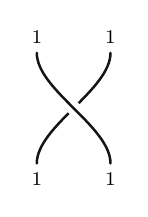
\begin{tikzpicture}[scale=.78,every node/.style={label}]
\ifstrequal{#1}{+}{
\draw[a,thickness={1}] (0.6,0)..controls(0.6,0.6)and(-0.6,1.2)..(-0.6,1.8);
\draw[a,over,thickness={1}] (-0.6,0)..controls(-0.6,0.6)and(0.6,1.2)..(0.6,1.8);
}{
\draw[a,thickness={1}] (-0.6,0)..controls(-0.6,0.6)and(0.6,1.2)..(0.6,1.8);
\draw[a,over,thickness={1}] (0.6,0)..controls(0.6,0.6)and(-0.6,1.2)..(-0.6,1.8);
}
\node[inputlabel]at(-0.6,0){$1$};
\node[inputlabel]at(0.6,0){$1$};
\node[outputlabel]at(-0.6,1.8){$1$};
\node[outputlabel]at(0.6,1.8){$1$};
\end{tikzpicture}}
\newcommand{\webdot}[1]{\begin{tikzpicture}[scale=.78,every node/.style={label}]
\draw[a,thickness={1}] (0,0)--(0,1.8);
\node[affinedot]at(0,0.9){$#1$};
\node[inputlabel]at(0,0){$1$};
\node[outputlabel]at(0,1.8){$1$};
\end{tikzpicture}}
% The five tree arguments are a,b,c,intermediate size,total size.
\newcommand{\webtreeleft}[5]{\begin{tikzpicture}[scale=.78,every node/.style={label}]
\draw[a,thickness={#5}] (0,1.9)--(0,2.4);
\draw[a,thickness={#3}] (1.1,0)..controls(1.1,1.1)and(0.6,1.55359)..(0,1.9);
\draw[a,thickness={#4}] (-0.55,1.1)..controls(-0.55,1.45)and(-0.42,1.657513)..(0,1.9);
\draw[a,thickness={#2}] (0,0)..controls(0,0.6)and(-0.13,0.857513)..(-0.55,1.1);
\draw[a,thickness={#1}] (-1.1,0)..controls(-1.1,0.6)and(-0.97,0.857513)..(-0.55,1.1);
\node[joint]at(0,1.9){};
\node[joint]at(-0.55,1.1){};
\node[inputlabel]at(-1.1,0){$#1$};
\node[inputlabel]at(0,0){$#2$};
\node[inputlabel]at(1.1,0){$#3$};
\node[outputlabel]at(0,2.4){$#5$};
\node[edgelabel,left=2pt]at(-0.57,1.54){$#4$};
\end{tikzpicture}}
\newcommand{\webtreeright}[5]{\begin{tikzpicture}[scale=.78,every node/.style={label}]
\draw[a,thickness={#5}] (0,1.9)--(0,2.4);
\draw[a,thickness={#1}] (-1.1,0)..controls(-1.1,1.1)and(-0.6,1.55359)..(0,1.9);
\draw[a,thickness={#4}] (0.55,1.1)..controls(0.55,1.45)and(0.42,1.657513)..(0,1.9);
\draw[a,thickness={#2}] (0,0)..controls(0,0.6)and(0.13,0.857513)..(0.55,1.1);
\draw[a,thickness={#3}] (1.1,0)..controls(1.1,0.6)and(0.97,0.857513)..(0.55,1.1);
\node[joint]at(0,1.9){};
\node[joint]at(0.55,1.1){};
\node[inputlabel]at(-1.1,0){$#1$};
\node[inputlabel]at(0,0){$#2$};
\node[inputlabel]at(1.1,0){$#3$};
\node[outputlabel]at(0,2.4){$#5$};
\node[edgelabel,right=2pt]at(0.57,1.54){$#4$};
\end{tikzpicture}}
% The ordinary three-edge splitter. The arguments are total,a,a+b,b.
\newcommand{\threebody}[4]{
\draw[a,thickness={#1}] (0,0)--(0,0.5);
\draw[a,thickness={#2}] (0,0.5)..controls(-0.6,0.84641)and(-1.1,1.3)..(-1.1,2.4);
\draw[a,thickness={#3}] (0,0.5)..controls(0.42,0.742487)and(0.55,0.95)..(0.55,1.3);
\draw[a,thickness={1}] (0.55,1.3)..controls(0.13,1.542487)and(0,1.8)..(0,2.4);
\draw[a,thickness={#4}] (0.55,1.3)..controls(0.97,1.542487)and(1.1,1.8)..(1.1,2.4);
\node[joint]at(0,0.5){};
\node[joint]at(0.55,1.3){};
\node[inputlabel]at(0,0){$#1$};
\node[outputlabel]at(-1.1,2.4){$#2$};
\node[outputlabel]at(0,2.4){$1$};
\node[outputlabel]at(1.1,2.4){$#4$};
\ifwebdetails\node[edgelabel,right=2pt]at(0.57,0.86){$#3$};\fi
}
\newcommand{\Bweb}[1][.72]{\begin{tikzpicture}[scale=#1,every node/.style={label}]
\threebody{N}{m}{m+1}{m}
\end{tikzpicture}}
\newcommand{\Btwo}[1][.72]{\begin{tikzpicture}[scale=#1,every node/.style={label}]
\threebody{5}{2}{3}{2}
\end{tikzpicture}}
% A positive one-strand winding, with the cut displayed.
\newcommand{\coilstrip}{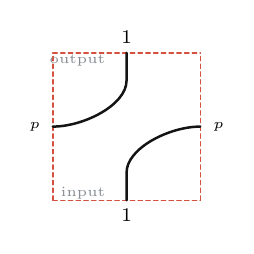
\begin{tikzpicture}[scale=.78,every node/.style={label}]
\draw[rim](-1.2,0)--(1.2,0) (-1.2,2.4)--(1.2,2.4);
\draw[cut](-1.2,0)--(-1.2,2.4) (1.2,0)--(1.2,2.4);
\draw[a,thickness={1}] (0,0)--(0,0.45)..controls(0,0.85)and(0.7,1.2)..(1.2,1.2);
\draw[a,thickness={1}] (-1.2,1.2)..controls(-0.7,1.2)and(0,1.55)..(0,1.95)--(0,2.4);
\node[inputlabel]at(0,0){$1$};
\node[outputlabel]at(0,2.4){$1$};
\node[seamlabel,left=2pt]at(-1.2,1.2){$p$};
\node[seamlabel,right=2pt]at(1.2,1.2){$p$};
\node[font=\tiny,text=webguide,anchor=east]at(-.2,.12){input};
\node[font=\tiny,text=webguide,anchor=east]at(-.2,2.28){output};
\end{tikzpicture}}

\newcommand{\coilannulus}{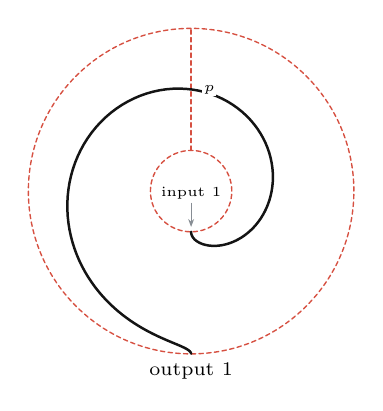
\begin{tikzpicture}[scale=.78,every node/.style={label}]
\begin{scope}[scale=.6625]
\draw[rim](0,0)circle(1) (0,0)circle(4);
\draw[cut](90:1)--(90:4);
\draw[a,thickness={1}]plot[domain=0:1,samples=151,variable=\t] ({-90+360*\t*\t*(3-2*\t)}:{1+3*\t});
\node[font=\tiny]at(0,-.05){input $1$};
\draw[draw=webguide,-{Stealth[length=1mm]},line width=.35pt](0,-.3)--(0,-.88);
\node[boundarylabel,anchor=north]at(0,-4){output $1$};
\node[seamlabel,right=2pt]at(0,2.5){$p$};
\end{scope}
\end{tikzpicture}}

\newcommand{\outermerge}{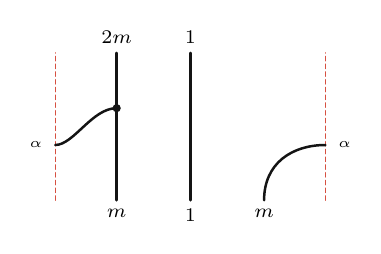
\begin{tikzpicture}[scale=.78,every node/.style={label}]
\draw[cut](-2.2,0)--(-2.2,2.4) (2.2,0)--(2.2,2.4);
\draw[a,thickness={m}] (-1.2,0)--(-1.2,1.5);
\draw[a,thickness={m}] (1.2,0)..controls(1.2,0.6)and(1.65,0.9)..(2.2,0.9);
\draw[a,thickness={m}] (-2.2,0.9)..controls(-1.9,0.9)and(-1.6,1.5)..(-1.2,1.5);
\draw[a,thickness={2*m}] (-1.2,1.5)--(-1.2,2.4);
\draw[a,thickness={1}] (0,0)--(0,2.4);
\node[joint]at(-1.2,1.5){};
\node[inputlabel]at(-1.2,0){$m$};
\node[inputlabel]at(0,0){$1$};
\node[inputlabel]at(1.2,0){$m$};
\node[outputlabel]at(-1.2,2.4){$2m$};
\node[outputlabel]at(0,2.4){$1$};
\node[seamlabel,left=2pt]at(-2.2,0.9){$\alpha$};
\node[seamlabel,right=2pt]at(2.2,0.9){$\alpha$};
\end{tikzpicture}}

\newcommand{\zeromerge}{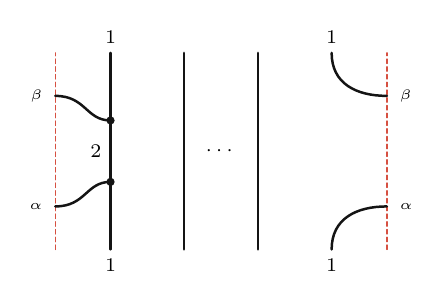
\begin{tikzpicture}[scale=.78,every node/.style={label}]
\draw[cut](-2.7,0)--(-2.7,3.2) (2.7,0)--(2.7,3.2);
\draw[a,thickness={1}] (-1.8,0)--(-1.8,1.1);
\draw[a] (-1.8,1.1)--(-1.8,2.1);
\draw[a,thickness={1}] (-1.8,2.1)--(-1.8,3.2);
\draw[a,thickness={1}] (1.8,0)..controls(1.8,0.5)and(2.2,0.7)..(2.7,0.7);
\draw[a,thickness={1}] (-2.7,0.7)..controls(-2.2,0.7)and(-2.2,1.1)..(-1.8,1.1);
\draw[a,thickness={1}] (-1.8,2.1)..controls(-2.2,2.1)and(-2.2,2.5)..(-2.7,2.5);
\draw[a,thickness={1}] (2.7,2.5)..controls(2.2,2.5)and(1.8,2.7)..(1.8,3.2);
\draw[a,thickness={1}] (-0.6,0)--(-0.6,3.2);
\draw[a,thickness={1}] (0.6,0)--(0.6,3.2);
\node[joint]at(-1.8,1.1){};
\node[joint]at(-1.8,2.1){};
\node[edgelabel,left=2pt]at(-1.8,1.6){$2$};
\node[edgelabel]at(0,1.6){$\cdots$};
\node[inputlabel]at(-1.8,0){$1$};
\node[inputlabel]at(1.8,0){$1$};
\node[outputlabel]at(-1.8,3.2){$1$};
\node[outputlabel]at(1.8,3.2){$1$};
\node[seamlabel,left=2pt]at(-2.7,0.7){$\alpha$};
\node[seamlabel,left=2pt]at(-2.7,2.5){$\beta$};
\node[seamlabel,right=2pt]at(2.7,0.7){$\alpha$};
\node[seamlabel,right=2pt]at(2.7,2.5){$\beta$};
\end{tikzpicture}}

\newcommand{\refinestrong}{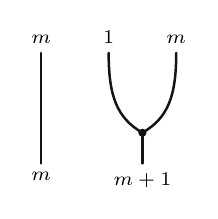
\begin{tikzpicture}[scale=.78,every node/.style={label}]
\draw[a,thickness={m}] (-1.1,0)--(-1.1,1.8);
\draw[a,thickness={m+1}] (0.55,0)--(0.55,0.5);
\draw[a,thickness={1}] (0.55,0.5)..controls(0.13,0.742487)and(0,1.1)..(0,1.8);
\draw[a,thickness={m}] (0.55,0.5)..controls(0.97,0.742487)and(1.1,1.1)..(1.1,1.8);
\node[joint]at(0.55,0.5){};
\node[outputlabel]at(-1.1,1.8){$m$};
\node[outputlabel]at(0,1.8){$1$};
\node[outputlabel]at(1.1,1.8){$m$};
\node[inputlabel]at(-1.1,0){$m$};
\node[inputlabel]at(0.55,0){$m+1$};
\end{tikzpicture}}

\newcommand{\refineweak}{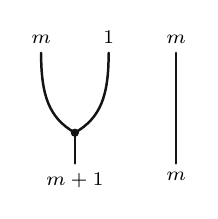
\begin{tikzpicture}[scale=.78,every node/.style={label}]
\draw[a,thickness={m}] (1.1,0)--(1.1,1.8);
\draw[a,thickness={m+1}] (-0.55,0)--(-0.55,0.5);
\draw[a,thickness={1}] (-0.55,0.5)..controls(-0.13,0.742487)and(0,1.1)..(0,1.8);
\draw[a,thickness={m}] (-0.55,0.5)..controls(-0.97,0.742487)and(-1.1,1.1)..(-1.1,1.8);
\node[joint]at(-0.55,0.5){};
\node[outputlabel]at(-1.1,1.8){$m$};
\node[outputlabel]at(0,1.8){$1$};
\node[outputlabel]at(1.1,1.8){$m$};
\node[inputlabel]at(1.1,0){$m$};
\node[inputlabel]at(-0.55,0){$m+1$};
\end{tikzpicture}}

\newcommand{\allthinTwo}{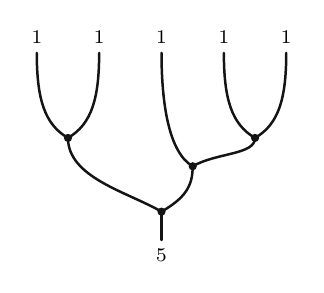
\begin{tikzpicture}[scale=.72,every node/.style={label}]
\draw[a] (0,0)--(0,0.5);
\draw[a] (0,0.5)..controls(-0.6,0.84641)and(-1.65,1.1)..(-1.65,1.8);
\draw[a] (0,0.5)..controls(0.42,0.742487)and(0.55,0.95)..(0.55,1.3);
\draw[a,thickness={1}] (0.55,1.3)..controls(0.13,1.542487)and(0,2.4)..(0,3.3);
\draw[a] (0.55,1.3)..controls(0.97,1.542487)and(1.65,1.5)..(1.65,1.8);
\draw[a,thickness={1}] (-1.65,1.8)..controls(-2.07,2.042487)and(-2.2,2.5)..(-2.2,3.3);
\draw[a,thickness={1}] (-1.65,1.8)..controls(-1.23,2.042487)and(-1.1,2.5)..(-1.1,3.3);
\draw[a,thickness={1}] (1.65,1.8)..controls(1.23,2.042487)and(1.1,2.5)..(1.1,3.3);
\draw[a,thickness={1}] (1.65,1.8)..controls(2.07,2.042487)and(2.2,2.5)..(2.2,3.3);
\node[joint]at(0,0.5){};
\node[joint]at(0.55,1.3){};
\node[joint]at(-1.65,1.8){};
\node[joint]at(1.65,1.8){};
\node[outputlabel]at(-2.2,3.3){$1$};
\node[outputlabel]at(-1.1,3.3){$1$};
\node[outputlabel]at(0,3.3){$1$};
\node[outputlabel]at(1.1,3.3){$1$};
\node[outputlabel]at(2.2,3.3){$1$};
\node[inputlabel]at(0,0){$5$};
\end{tikzpicture}}

\newcommand{\webinversepair}{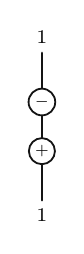
\begin{tikzpicture}[scale=.78,every node/.style={label}]
\draw[a,thickness={1}] (0,0)--(0,2.4);
\node[affinedot]at(0,0.8){$+$};
\node[affinedot]at(0,1.6){$-$};
\node[inputlabel]at(0,0){$1$};
\node[outputlabel]at(0,2.4){$1$};
\end{tikzpicture}}
\newcommand{\webinversepairtwo}{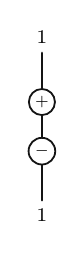
\begin{tikzpicture}[scale=.78,every node/.style={label}]
\draw[a,thickness={1}] (0,0)--(0,2.4);
\node[affinedot]at(0,0.8){$-$};
\node[affinedot]at(0,1.6){$+$};
\node[inputlabel]at(0,0){$1$};
\node[outputlabel]at(0,2.4){$1$};
\end{tikzpicture}}

% Composite strip and annular diagrams.
% Shared drawing styles. Label gaps and line weights are physical dimensions,
% so they remain the same in large figures and in small equation diagrams.
\tikzset{
a/.style={draw=webink,line width=.9pt,line cap=round,line join=round},
usual/.style={a}, web/.style={a},
marked/.style={draw=webhighlight,line width=1.2pt,line cap=round,line join=round},
cut/.style={draw=webboundary,dash pattern=on 1.6pt off 1.2pt,line width=.5pt},
rim/.style={draw=webboundary,dash pattern=on 1.6pt off 1.2pt,line width=.5pt},
gluing/.style={draw=webguide,line width=.4pt},
joint/.style={circle,fill=webink,inner sep=1.05pt,outer sep=0pt},
dot/.style={joint},
label/.style={font=\scriptsize,inner sep=1.3pt,outer sep=2pt},
edgelabel/.style={label,outer sep=0pt},
boundarylabel/.style={label,outer sep=2pt},
inputlabel/.style={boundarylabel,anchor=north},
outputlabel/.style={boundarylabel,anchor=south},
affinedot/.style={circle,draw=webink,fill=white,line width=.65pt,
font=\tiny,inner sep=1pt,outer sep=0pt},
seamlabel/.style={font=\tiny,fill=white,inner sep=.7pt},
directed/.style={postaction={decorate},decoration={markings,
mark=at position .72 with {\arrow{Stealth[length=1.5mm,width=1.1mm]}}}}
}
% Place an outer boundary label at a fixed distance from the rim.
\newcommand{\annularlabel}[3]{%
\node[boundarylabel,anchor={#1+180}]at(#1:#2){$#3$};%
}
\newcommand{\annularinputlabel}[3]{%
\node[boundarylabel,anchor={#1}]at(#1:#2){$#3$};%
}

% Carrier geometry: shorten only the empty middle intervals; widths,
% vertex neighborhoods, label sizes and line weights are unchanged.
\newcommand{\WideRbody}[6]{%
\webcuts{-3.25}{3.25}{8.2}
\draw[a,thickness={#1}] (0,0)--(0,0.6);
\draw[a,thickness={#2}] (0,0.6)..controls(-0.433013,0.85)and(-1.6,2.58)..(-1.6,3);
\draw[a,thickness={#6}] (0,0.6)..controls(0.433013,0.85)and(0.65,0.88)..(0.65,1.3);
\draw[a,thickness={1}] (0.65,1.3)..controls(0.216987,1.55)and(-1,4.3)..(-1,5.4);
\draw[a,thickness={#2}] (0.65,1.3)..controls(1.083013,1.55)and(1.8,2.4)..(3.25,2.4);
\draw[a,thickness={#2}] (-3.25,2.4)..controls(-2.6,2.4)and(-2.02,3)..(-1.6,3);
\draw[a,thickness={#4}] (-1.6,3)--(-1.6,4.1);
\draw[a,thickness={#2}] (-1.6,4.1)..controls(-1.6,4.52)and(-2,4.98)..(-2,5.4);
\draw[a,thickness={#2}] (-1.6,4.1)..controls(-2.02,4.1)and(-2.8,4.5)..(-3.25,4.5);
\draw[a,thickness={#2}] (3.25,4.5)..controls(2.6,4.5)and(2,4.5)..(2,5.4);
\draw[marked] (-2,5.4)--(-2,6.8);
\draw[a,thickness={#3}] (-2,5.4)--(-1,5.4);
\draw[a,thickness={#3}] (2,5.4)--(0,5.4);
\draw[marked] (2,5.4)--(2,6.8);
\draw[a,thickness={#2}] (-1,5.4)--(0,5.4);
\draw[a,thickness={#5}] (0,5.4)--(0,6.8);
\draw[a,thickness={#3}] (0,6.8)--(-2,6.8);
\draw[a,thickness={#2}] (0,6.8)--(1,6.8);
\draw[a,thickness={1}] (1,6.8)..controls(1,7.6)and(0,7.6)..(0,8.2);
\draw[a,thickness={#3}] (1,6.8)--(2,6.8);
\draw[a,thickness={#2}] (-2,6.8)--(-2,8.2);
\draw[a,thickness={#2}] (2,6.8)--(2,8.2);
\node[joint]at(0,0.6){};
\node[joint]at(0.65,1.3){};
\node[joint]at(-1.6,3){};
\node[joint]at(-1.6,4.1){};
\node[joint]at(-2,5.4){};
\node[joint]at(2,5.4){};
\node[joint]at(-1,5.4){};
\node[joint]at(0,5.4){};
\node[joint]at(0,6.8){};
\node[joint]at(1,6.8){};
\node[joint]at(-2,6.8){};
\node[joint]at(2,6.8){};
\node[inputlabel]at(0,0){$#1$};
\node[outputlabel]at(-2,8.2){$#2$};
\node[outputlabel]at(0,8.2){$1$};
\node[outputlabel]at(2,8.2){$#2$};
\ifwebdetails
\node[edgelabel,anchor=east]at(-1.82,1.8){$#2$};
\node[edgelabel,anchor=west]at(1.7,1.8){$#2$};
\node[edgelabel,anchor=west]at(0.72,0.82){$#6$};
\node[edgelabel,anchor=east]at(-1.82,3.55){$#4$};
\node[edgelabel,anchor=west]at(2.25,4.8){$#2$};
\node[edgelabel,anchor=east]at(-2.22,6.1){$1$};
\node[edgelabel,anchor=west]at(2.22,6.1){$1$};
\node[edgelabel,anchor=west]at(0.22,6.1){$#5$};
\fi
\ifwebdetails
\node[seamlabel,anchor=east]at(-3.35,2.57){$\alpha$};
\node[seamlabel,anchor=west]at(3.35,2.57){$\alpha$};
\node[seamlabel,anchor=east]at(-3.35,4.67){$\beta$};
\node[seamlabel,anchor=west]at(3.35,4.67){$\beta$};
\fi
}

\newcommand{\WideRannotatedBody}[6]{%
\webcuts{-3.25}{3.25}{8.6}
\draw[a,thickness={#1}] (0,0)--(0,0.6);
\draw[a,thickness={#2}] (0,0.6)..controls(-0.433013,0.85)and(-1.6,2.58)..(-1.6,3);
\draw[a,thickness={#6}] (0,0.6)..controls(0.433013,0.85)and(0.65,0.88)..(0.65,1.3);
\draw[a,thickness={1}] (0.65,1.3)..controls(0.216987,1.55)and(-1,4.3)..(-1,5.4);
\draw[a,thickness={#2}] (0.65,1.3)..controls(1.083013,1.55)and(1.8,2.4)..(3.25,2.4);
\draw[a,thickness={#2}] (-3.25,2.4)..controls(-2.6,2.4)and(-2.02,3)..(-1.6,3);
\draw[a,thickness={#4}] (-1.6,3)--(-1.6,4.1);
\draw[a,thickness={#2}] (-1.6,4.1)..controls(-1.6,4.52)and(-2,4.98)..(-2,5.4);
\draw[a,thickness={#2}] (-1.6,4.1)..controls(-2.02,4.1)and(-2.8,4.5)..(-3.25,4.5);
\draw[a,thickness={#2}] (3.25,4.5)..controls(2.6,4.5)and(2,4.5)..(2,5.4);
\draw[marked] (-2,5.4)--(-2,7.2);
\draw[a,thickness={#3}] (-2,5.4)--(-1,5.4);
\draw[a,thickness={#3}] (2,5.4)--(0,5.4);
\draw[marked] (2,5.4)--(2,7.2);
\draw[a,thickness={#2}] (-1,5.4)--(0,5.4);
\draw[a,thickness={#5}] (0,5.4)--(0,7.2);
\draw[a,thickness={#3}] (0,7.2)--(-2,7.2);
\draw[a,thickness={#2}] (0,7.2)--(1,7.2);
\draw[a,thickness={1}] (1,7.2)..controls(1,8)and(0,8)..(0,8.6);
\draw[a,thickness={#3}] (1,7.2)--(2,7.2);
\draw[a,thickness={#2}] (-2,7.2)--(-2,8.6);
\draw[a,thickness={#2}] (2,7.2)--(2,8.6);
\node[joint]at(0,0.6){};
\node[joint]at(0.65,1.3){};
\node[joint]at(-1.6,3){};
\node[joint]at(-1.6,4.1){};
\node[joint]at(-2,5.4){};
\node[joint]at(2,5.4){};
\node[joint]at(-1,5.4){};
\node[joint]at(0,5.4){};
\node[joint]at(0,7.2){};
\node[joint]at(1,7.2){};
\node[joint]at(-2,7.2){};
\node[joint]at(2,7.2){};
\node[inputlabel]at(0,0){$#1$};
\node[outputlabel]at(-2,8.6){$#2$};
\node[outputlabel]at(0,8.6){$1$};
\node[outputlabel]at(2,8.6){$#2$};
\ifwebdetails
\node[edgelabel,anchor=east]at(-1.82,1.8){$#2$};
\node[edgelabel,anchor=west]at(1.7,1.8){$#2$};
\node[edgelabel,anchor=west]at(0.72,0.82){$#6$};
\node[edgelabel,anchor=east]at(-1.82,3.55){$#4$};
\node[edgelabel,anchor=west]at(2.25,4.8){$#2$};
\node[edgelabel,anchor=east]at(-2.22,6.3){$1$};
\node[edgelabel,anchor=west]at(2.22,6.3){$1$};
\node[edgelabel,anchor=west]at(0.22,6.3){$#5$};
\fi
\ifwebdetails
\node[seamlabel,anchor=east]at(-3.35,2.57){$\alpha$};
\node[seamlabel,anchor=west]at(3.35,2.57){$\alpha$};
\node[seamlabel,anchor=east]at(-3.35,4.67){$\beta$};
\node[seamlabel,anchor=west]at(3.35,4.67){$\beta$};
\fi
\draw[draw=webguide,line width=.35pt](-3.7,1.9)--(-3.4,1.9);
\node[anchor=east,font=\small]at(-3.85,1.9){$(a)\quad V=(m,1,m)$};
\draw[draw=webguide,line width=.35pt](-3.7,3.55)--(-3.4,3.55);
\node[anchor=east,font=\small]at(-3.85,3.55){$(b)\quad J=(2m,1)$};
\draw[draw=webguide,line width=.35pt](-3.7,5.4)--(-3.4,5.4);
\node[anchor=east,font=\small]at(-3.85,5.4){$(c)\quad L=(1,m-1,1,m-1,1)$};
\draw[draw=webguide,line width=.35pt](-3.7,6.3)--(-3.4,6.3);
\node[anchor=east,font=\small]at(-3.85,6.3){$(d)\quad K=(1,2m-1,1)$};
\draw[draw=webguide,line width=.35pt](-3.7,7.2)--(-3.4,7.2);
\node[anchor=east,font=\small]at(-3.85,7.2){$(e)\quad L=(1,m-1,1,m-1,1)$};
\draw[draw=webguide,line width=.35pt](-3.7,8.6)--(-3.4,8.6);
\node[anchor=east,font=\small]at(-3.85,8.6){$(f)\quad V=(m,1,m)$};
}

\newcommand{\WideRannBody}[6]{%
\begin{scope}[scale=1.05]
\draw[rim](0,0)circle(1) (0,0)circle(4);
\draw[cut](90:1)--(90:4);
\draw[a,rounded corners=3pt,thickness={#1}] (-90:1)..controls(-90:1.15)and(-105:1.25)..(-105:1.45);
\draw[a,rounded corners=3pt,thickness={#6}] (-105:1.45) arc[start angle=-105,end angle=-75,radius=1.45];
\draw[a,rounded corners=3pt,thickness={#2}] (-105:1.45) arc[start angle=-105,end angle=-180,radius=1.45]--(-180:1.9);
\draw[a,rounded corners=3pt,thickness={#2}] (-75:1.45) arc[start angle=-75,end angle=-45,radius=1.45]--(-45:1.9) arc[start angle=-45,end angle=180,radius=1.9];
\draw[a,rounded corners=3pt,thickness={#4}] (-180:1.9)--(-180:2.2);
\draw[a,rounded corners=3pt,thickness={#2}] (-180:2.2) arc[start angle=-180,end angle=-111,radius=2.2]--(-111:2.45);
\draw[a,rounded corners=3pt,thickness={#2}] (-180:2.2) arc[start angle=-180,end angle=-429,radius=2.2]--(-69:2.45);
\draw[a,rounded corners=3pt,thickness={1}] (-75:1.45)..controls(-75:1.85)and(-100.5:2.05)..(-100.5:2.45);
\draw[a,rounded corners=3pt,thickness={#3}] (-111:2.45) arc[start angle=-111,end angle=-100.5,radius=2.45];
\draw[a,rounded corners=3pt,thickness={#2}] (-100.5:2.45) arc[start angle=-100.5,end angle=-90,radius=2.45];
\draw[a,rounded corners=3pt,thickness={#3}] (-69:2.45) arc[start angle=-69,end angle=-90,radius=2.45];
\draw[a,rounded corners=3pt,thickness={#5}] (-90:2.45)--(-90:3.55);
\draw[a,rounded corners=3pt,thickness={#2}] (-90:3.55) arc[start angle=-90,end angle=-79.5,radius=3.55];
\draw[marked,rounded corners=3pt] (-111:2.45)--(-111:3.55);
\draw[marked,rounded corners=3pt] (-69:2.45)--(-69:3.55);
\draw[a,rounded corners=3pt,thickness={#3}] (-90:3.55) arc[start angle=-90,end angle=-111,radius=3.55];
\draw[a,rounded corners=3pt,thickness={#3}] (-79.5:3.55) arc[start angle=-79.5,end angle=-69,radius=3.55];
\draw[a,rounded corners=3pt,thickness={#2}] (-111:3.55) arc[start angle=-111,end angle=-210,radius=3.55]--(-210:4);
\draw[a,rounded corners=3pt,thickness={#2}] (-69:3.55) arc[start angle=-69,end angle=30,radius=3.55]--(30:4);
\draw[a,thickness={1}] (-79.5:3.55)..controls(0.692039,-3.73391)and(0,-3.7525)..(-90:4);
\node[joint]at(-105:1.45){};
\node[joint]at(-75:1.45){};
\node[joint]at(-180:1.9){};
\node[joint]at(-180:2.2){};
\node[joint]at(-111:2.45){};
\node[joint]at(-69:2.45){};
\node[joint]at(-100.5:2.45){};
\node[joint]at(-90:2.45){};
\node[joint]at(-90:3.55){};
\node[joint]at(-79.5:3.55){};
\node[joint]at(-111:3.55){};
\node[joint]at(-69:3.55){};
\node[boundarylabel]at(0,0){$#1$};
\annularlabel{-210}{4}{#2}
\annularlabel{-90}{4}{1}
\annularlabel{30}{4}{#2}
\draw[draw=webguide,-{Stealth[length=1mm]},line width=.35pt](0,-.3)--(0,-.88);
\end{scope}
}

\newcommand{\WideVbody}[3]{%
\webcuts{-2.2}{2.2}{5.6}
\draw[a,thickness={#1}] (0,0)--(0,0.6);
\draw[a,thickness={#2}] (0,0.6)..controls(-0.433013,0.85)and(-1,1.88)..(-1,2.3);
\draw[a,thickness={#3}] (0,0.6)..controls(0.433013,0.85)and(1.4,1.5)..(2.2,1.5);
\draw[a,thickness={#3}] (-2.2,1.5)..controls(-1.6,1.5)and(-1.42,2.3)..(-1,2.3);
\draw[a,thickness={#1}] (-1,2.3)--(-1,3.3);
\draw[a,thickness={#2}] (-1,3.3)..controls(-1,3.72)and(-0.433013,4.75)..(0,5);
\draw[a,thickness={#3}] (-1,3.3)..controls(-1.42,3.3)and(-1.6,4.1)..(-2.2,4.1);
\draw[a,thickness={#3}] (2.2,4.1)..controls(1.4,4.1)and(0.433013,4.75)..(0,5);
\draw[a,thickness={#1}] (0,5)--(0,5.6);
\node[joint]at(0,0.6){};
\node[joint]at(-1,2.3){};
\node[joint]at(-1,3.3){};
\node[joint]at(0,5){};
\node[inputlabel]at(0,0){$#1$};
\node[outputlabel]at(0,5.6){$#1$};
\ifwebdetails
\node[edgelabel,anchor=east]at(-1.22,1.3){$#2$};
\node[edgelabel,anchor=south]at(1.1,1.6){$#3$};
\node[edgelabel,anchor=east]at(-1.22,2.8){$#1$};
\node[edgelabel,anchor=east]at(-1.22,4.3){$#2$};
\node[edgelabel,anchor=north]at(1.1,4){$#3$};
\fi
\ifwebdetails
\node[seamlabel,anchor=east]at(-2.3,1.67){$\alpha$};
\node[seamlabel,anchor=west]at(2.3,1.67){$\alpha$};
\node[seamlabel,anchor=east]at(-2.3,4.27){$\beta$};
\node[seamlabel,anchor=west]at(2.3,4.27){$\beta$};
\fi
}

\newcommand{\WideVrefbody}[3]{%
\webcuts{-2.2}{2.2}{8}
\draw[a,thickness={#1}] (0,0)--(0,0.6);
\draw[a,thickness={#2}] (0,0.6)..controls(-0.433013,0.85)and(-1,1.88)..(-1,2.3);
\draw[a,thickness={#3}] (0,0.6)..controls(0.433013,0.85)and(1.4,1.5)..(2.2,1.5);
\draw[a,thickness={#3}] (-2.2,1.5)..controls(-1.6,1.5)and(-1.42,2.3)..(-1,2.3);
\draw[a,thickness={#1}] (-1,2.3)--(-1,3.3);
\draw[a,thickness={#2}] (-1,3.3)..controls(-1,3.72)and(-0.433013,4.75)..(0,5);
\draw[a,thickness={#3}] (-1,3.3)..controls(-1.42,3.3)and(-1.6,4.1)..(-2.2,4.1);
\draw[a,thickness={#3}] (2.2,4.1)..controls(1.4,4.1)and(0.433013,4.75)..(0,5);
\draw[a,thickness={#1}] (0,5)--(0,5.6);
\node[joint]at(0,0.6){};
\node[joint]at(-1,2.3){};
\node[joint]at(-1,3.3){};
\node[joint]at(0,5){};
\node[inputlabel]at(0,0){$#1$};
\ifwebdetails
\node[edgelabel,anchor=east]at(-1.22,1.3){$#2$};
\node[edgelabel,anchor=south]at(1.1,1.6){$#3$};
\node[edgelabel,anchor=east]at(-1.22,2.8){$#1$};
\node[edgelabel,anchor=east]at(-1.22,4.3){$#2$};
\node[edgelabel,anchor=north]at(1.1,4){$#3$};
\else
\node[edgelabel,anchor=east]at(-1.22,1.3){$#2$};
\node[edgelabel,anchor=south]at(1.1,1.6){$#3$};
\fi
\ifwebdetails
\node[seamlabel,anchor=east]at(-2.3,1.67){$\alpha$};
\node[seamlabel,anchor=west]at(2.3,1.67){$\alpha$};
\node[seamlabel,anchor=east]at(-2.3,4.27){$\beta$};
\node[seamlabel,anchor=west]at(2.3,4.27){$\beta$};
\fi
}

\newcommand{\WideVannBody}[3]{%
\begin{scope}[scale=0.75]
\draw[rim](0,0)circle(1) (0,0)circle(4);
\draw[cut](90:1)--(90:4);
\draw[a,rounded corners=3pt,thickness={#1}] (-90:1)--(-90:1.25);
\draw[a,rounded corners=3pt,thickness={#2}] (-90:1.25) arc[start angle=-90,end angle=-180,radius=1.25]--(-180:1.9);
\draw[a,rounded corners=3pt,thickness={#3}] (-90:1.25)--(-90:1.9) arc[start angle=-90,end angle=180,radius=1.9];
\draw[a,rounded corners=3pt,thickness={#1}] (-180:1.9)--(-180:2.2);
\draw[a,rounded corners=3pt,thickness={#2}] (-180:2.2)--(-180:3.55) arc[start angle=-180,end angle=-90,radius=3.55];
\draw[a,rounded corners=3pt,thickness={#3}] (-180:2.2) arc[start angle=-180,end angle=-450,radius=2.2]--(-90:3.55);
\draw[a,rounded corners=3pt,thickness={#1}] (-90:3.55)--(-90:4);
\node[joint]at(-90:1.25){};
\node[joint]at(-180:1.9){};
\node[joint]at(-180:2.2){};
\node[joint]at(-90:3.55){};
\node[boundarylabel]at(0,0){$#1$};
\annularlabel{-90}{4}{#1}
\draw[draw=webguide,-{Stealth[length=1mm]},line width=.35pt](0,-.3)--(0,-.88);
\end{scope}
}

\newcommand{\WideEnone}[9]{%
\webcuts{-2.6}{2.6}{7.5}
\draw[a,thickness={#1}] (0,0)--(0,0.6);
\draw[a,thickness={#2}] (0,0.6)..controls(-0.433013,0.85)and(-1.2,2.38)..(-1.2,2.8);
\draw[a,thickness={#3}] (0,0.6)..controls(0.433013,0.85)and(1.6,2.2)..(2.6,2.2);
\draw[a,thickness={#3}] (-2.6,2.2)..controls(-2,2.2)and(-1.62,2.8)..(-1.2,2.8);
\draw[a,thickness={#1}] (-1.2,2.8)--(-1.2,3.7);
\draw[a,thickness={#3}] (-1.2,3.7)..controls(-1.62,3.7)and(-2,4.3)..(-2.6,4.3);
\draw[a,thickness={#3}] (2.6,4.3)..controls(2,4.3)and(1.2,4.3)..(1.2,5.2);
\draw[a,thickness={#2}] (-1.2,3.7)..controls(-1.2,4.12)and(-1.2,4.78)..(-1.2,5.2);
\draw[marked] (-1.2,5.2)--(-1.2,6.7);
\draw[a,thickness={#4}] (-1.2,5.2)--(1.2,5.2);
\draw[a,thickness={#1-1}] (1.2,5.2)--(1.2,6.7);
\draw[a,thickness={#6}] (1.2,6.7)--(-1.2,6.7);
\draw[a,thickness={#7}] (1.2,6.7)..controls(1.591918,6.926274)and(2,7.05)..(2,7.5);
\draw[a,thickness={#5}] (-1.2,6.7)..controls(-1.2,7.152548)and(-2,7.05)..(-2,7.5);
\node[joint]at(0,0.6){};
\node[joint]at(-1.2,2.8){};
\node[joint]at(-1.2,3.7){};
\node[joint]at(1.2,6.7){};
\node[joint]at(-1.2,6.7){};
\node[joint]at(-1.2,5.2){};
\node[joint]at(1.2,5.2){};
\node[inputlabel]at(0,0){$#1$};
\node[outputlabel]at(-2,7.5){$#5$};
\node[outputlabel]at(2,7.5){$#7$};
\ifwebdetails
\node[edgelabel,anchor=east]at(-1.4,1.5){$#2$};
\node[edgelabel,anchor=north]at(1.4,1.4){$#3$};
\node[edgelabel,anchor=east]at(-1.4,3.2){$#1$};
\node[edgelabel,anchor=east]at(-1.4,5.95){$1$};
\node[edgelabel,anchor=east]at(1,4.75){$#3$};
\node[edgelabel,anchor=west]at(1.42,5.95){$N-1$};
\else
\node[edgelabel,anchor=east]at(-1.4,1.5){$#2$};
\node[edgelabel,anchor=west,xshift=2pt]at(2.6,1.15){$#3$};
\fi
\ifwebdetails
\node[seamlabel,anchor=east]at(-2.7,2.37){$\alpha$};
\node[seamlabel,anchor=west]at(2.7,2.37){$\alpha$};
\node[seamlabel,anchor=east]at(-2.7,4.47){$\beta$};
\node[seamlabel,anchor=west]at(2.7,4.47){$\beta$};
\fi
}

\newcommand{\WideEnoneZero}[9]{%
\webcuts{-2.6}{2.6}{7.5}
\draw[a,thickness={#1}] (0,0)--(0,0.6);
\draw[a,thickness={#2}] (0,0.6)..controls(-0.433013,0.85)and(-1.2,2.38)..(-1.2,2.8);
\draw[a,thickness={#3}] (0,0.6)..controls(0.433013,0.85)and(1.6,2.2)..(2.6,2.2);
\draw[a,thickness={#3}] (-2.6,2.2)..controls(-2,2.2)and(-1.62,2.8)..(-1.2,2.8);
\draw[a,thickness={#1}] (-1.2,2.8)--(-1.2,3.7);
\draw[a,thickness={#3}] (-1.2,3.7)..controls(-1.62,3.7)and(-2,4.3)..(-2.6,4.3);
\draw[a,thickness={#3}] (2.6,4.3)..controls(2,4.3)and(1.2,4.3)..(1.2,6.7);
\draw[marked] (-1.2,3.7)..controls(-1.2,4.12)and(-1.2,6.4375)..(-1.2,6.7);
\draw[a,thickness={#6}] (1.2,6.7)--(-1.2,6.7);
\draw[a,thickness={#7}] (1.2,6.7)..controls(1.591918,6.926274)and(2,7.05)..(2,7.5);
\draw[a,thickness={#5}] (-1.2,6.7)..controls(-1.2,7.152548)and(-2,7.05)..(-2,7.5);
\node[joint]at(0,0.6){};
\node[joint]at(-1.2,2.8){};
\node[joint]at(-1.2,3.7){};
\node[joint]at(1.2,6.7){};
\node[joint]at(-1.2,6.7){};
\node[inputlabel]at(0,0){$#1$};
\node[outputlabel]at(-2,7.5){$#5$};
\node[outputlabel]at(2,7.5){$#7$};
\ifwebdetails
\node[edgelabel,anchor=east]at(-1.4,1.5){$#2$};
\node[edgelabel,anchor=north]at(1.4,1.4){$#3$};
\node[edgelabel,anchor=east]at(-1.4,3.2){$#1$};
\node[edgelabel,anchor=east]at(-1.4,5.95){$1$};
\node[edgelabel,anchor=east]at(1,4.75){$#3$};
\else
\node[edgelabel,anchor=east]at(-1.4,1.5){$#2$};
\node[edgelabel,anchor=west,xshift=2pt]at(2.6,1.15){$#3$};
\fi
\ifwebdetails
\node[seamlabel,anchor=east]at(-2.7,2.37){$\alpha$};
\node[seamlabel,anchor=west]at(2.7,2.37){$\alpha$};
\node[seamlabel,anchor=east]at(-2.7,4.47){$\beta$};
\node[seamlabel,anchor=west]at(2.7,4.47){$\beta$};
\fi
}

\newcommand{\WideEleft}[9]{%
\webcuts{-2.6}{2.6}{8.8}
\draw[a,thickness={#1}] (0,0)--(0,0.6);
\draw[a,thickness={#2}] (0,0.6)..controls(-0.433013,0.85)and(-1.2,2.38)..(-1.2,2.8);
\draw[a,thickness={#3}] (0,0.6)..controls(0.433013,0.85)and(1.6,2.2)..(2.6,2.2);
\draw[a,thickness={#3}] (-2.6,2.2)..controls(-2,2.2)and(-1.62,2.8)..(-1.2,2.8);
\draw[a,thickness={#1}] (-1.2,2.8)--(-1.2,3.7);
\draw[a,thickness={#3}] (-1.2,3.7)..controls(-1.62,3.7)and(-2,4.3)..(-2.6,4.3);
\draw[a,thickness={#3}] (2.6,4.3)..controls(2,4.3)and(1.2,4.3)..(1.2,5.2);
\draw[a,thickness={#2}] (-1.2,3.7)..controls(-1.2,4.12)and(-1.2,4.78)..(-1.2,5.2);
\draw[marked] (-1.2,5.2)--(-1.2,6.7);
\draw[a,thickness={#4}] (-1.2,5.2)--(1.2,5.2);
\draw[a,thickness={#1-1}] (1.2,5.2)--(1.2,6.7);
\draw[a,thickness={#6}] (1.2,6.7)--(-1.2,6.7);
\draw[a,thickness={#7}] (1.2,6.7)--(1.2,7.5);
\draw[a,thickness={#5}] (-1.2,6.7)--(-1.2,7.5);
\draw[a,thickness={#9}] (-1.2,7.5)..controls(-1.719615,7.8)and(-2,8.35)..(-2,8.8);
\draw[a,thickness={1}] (-1.2,7.5)..controls(-0.680385,7.8)and(0,8.35)..(0,8.8);
\draw[a,thickness={#9}] (1.2,7.5)..controls(1.2,8.1)and(2,8.35)..(2,8.8);
\node[joint]at(0,0.6){};
\node[joint]at(-1.2,2.8){};
\node[joint]at(-1.2,3.7){};
\node[joint]at(1.2,6.7){};
\node[joint]at(-1.2,6.7){};
\node[joint]at(-1.2,5.2){};
\node[joint]at(1.2,5.2){};
\node[joint]at(-1.2,7.5){};
\node[inputlabel]at(0,0){$#1$};
\node[outputlabel]at(-2,8.8){$#9$};
\node[outputlabel]at(0,8.8){$1$};
\node[outputlabel]at(2,8.8){$#9$};
\ifwebdetails
\node[edgelabel,anchor=east]at(-1.4,1.5){$#2$};
\node[edgelabel,anchor=north]at(1.4,1.4){$#3$};
\node[edgelabel,anchor=east]at(-1.4,3.2){$#1$};
\node[edgelabel,anchor=east]at(-1.4,5.95){$1$};
\node[edgelabel,anchor=east]at(1,4.75){$#3$};
\node[edgelabel,anchor=west]at(1.42,5.95){$N-1$};
\else
\node[edgelabel,anchor=east]at(-1.4,1.5){$#2$};
\node[edgelabel,anchor=west,xshift=2pt]at(2.6,1.15){$#3$};
\fi
\ifwebdetails
\node[seamlabel,anchor=east]at(-2.7,2.37){$\alpha$};
\node[seamlabel,anchor=west]at(2.7,2.37){$\alpha$};
\node[seamlabel,anchor=east]at(-2.7,4.47){$\beta$};
\node[seamlabel,anchor=west]at(2.7,4.47){$\beta$};
\fi
}

\newcommand{\WideEleftZero}[9]{%
\webcuts{-2.6}{2.6}{8.8}
\draw[a,thickness={#1}] (0,0)--(0,0.6);
\draw[a,thickness={#2}] (0,0.6)..controls(-0.433013,0.85)and(-1.2,2.38)..(-1.2,2.8);
\draw[a,thickness={#3}] (0,0.6)..controls(0.433013,0.85)and(1.6,2.2)..(2.6,2.2);
\draw[a,thickness={#3}] (-2.6,2.2)..controls(-2,2.2)and(-1.62,2.8)..(-1.2,2.8);
\draw[a,thickness={#1}] (-1.2,2.8)--(-1.2,3.7);
\draw[a,thickness={#3}] (-1.2,3.7)..controls(-1.62,3.7)and(-2,4.3)..(-2.6,4.3);
\draw[a,thickness={#3}] (2.6,4.3)..controls(2,4.3)and(1.2,4.3)..(1.2,6.7);
\draw[marked] (-1.2,3.7)..controls(-1.2,4.12)and(-1.2,6.4375)..(-1.2,6.7);
\draw[a,thickness={#6}] (1.2,6.7)--(-1.2,6.7);
\draw[a,thickness={#7}] (1.2,6.7)--(1.2,7.5);
\draw[a,thickness={#5}] (-1.2,6.7)--(-1.2,7.5);
\draw[a,thickness={#9}] (-1.2,7.5)..controls(-1.719615,7.8)and(-2,8.35)..(-2,8.8);
\draw[a,thickness={1}] (-1.2,7.5)..controls(-0.680385,7.8)and(0,8.35)..(0,8.8);
\draw[a,thickness={#9}] (1.2,7.5)..controls(1.2,8.1)and(2,8.35)..(2,8.8);
\node[joint]at(0,0.6){};
\node[joint]at(-1.2,2.8){};
\node[joint]at(-1.2,3.7){};
\node[joint]at(1.2,6.7){};
\node[joint]at(-1.2,6.7){};
\node[joint]at(-1.2,7.5){};
\node[inputlabel]at(0,0){$#1$};
\node[outputlabel]at(-2,8.8){$#9$};
\node[outputlabel]at(0,8.8){$1$};
\node[outputlabel]at(2,8.8){$#9$};
\ifwebdetails
\node[edgelabel,anchor=east]at(-1.4,1.5){$#2$};
\node[edgelabel,anchor=north]at(1.4,1.4){$#3$};
\node[edgelabel,anchor=east]at(-1.4,3.2){$#1$};
\node[edgelabel,anchor=east]at(-1.4,5.95){$1$};
\node[edgelabel,anchor=east]at(1,4.75){$#3$};
\else
\node[edgelabel,anchor=east]at(-1.4,1.5){$#2$};
\node[edgelabel,anchor=west,xshift=2pt]at(2.6,1.15){$#3$};
\fi
\ifwebdetails
\node[seamlabel,anchor=east]at(-2.7,2.37){$\alpha$};
\node[seamlabel,anchor=west]at(2.7,2.37){$\alpha$};
\node[seamlabel,anchor=east]at(-2.7,4.47){$\beta$};
\node[seamlabel,anchor=west]at(2.7,4.47){$\beta$};
\fi
}

\newcommand{\WideEright}[9]{%
\webcuts{-2.6}{2.6}{8.8}
\draw[a,thickness={#1}] (0,0)--(0,0.6);
\draw[a,thickness={#2}] (0,0.6)..controls(-0.433013,0.85)and(-1.2,2.38)..(-1.2,2.8);
\draw[a,thickness={#3}] (0,0.6)..controls(0.433013,0.85)and(1.6,2.2)..(2.6,2.2);
\draw[a,thickness={#3}] (-2.6,2.2)..controls(-2,2.2)and(-1.62,2.8)..(-1.2,2.8);
\draw[a,thickness={#1}] (-1.2,2.8)--(-1.2,3.7);
\draw[a,thickness={#3}] (-1.2,3.7)..controls(-1.62,3.7)and(-2,4.3)..(-2.6,4.3);
\draw[a,thickness={#3}] (2.6,4.3)..controls(2,4.3)and(1.2,4.3)..(1.2,5.2);
\draw[a,thickness={#2}] (-1.2,3.7)..controls(-1.2,4.12)and(-1.2,4.78)..(-1.2,5.2);
\draw[marked] (-1.2,5.2)--(-1.2,6.7);
\draw[a,thickness={#4}] (-1.2,5.2)--(1.2,5.2);
\draw[a,thickness={#1-1}] (1.2,5.2)--(1.2,6.7);
\draw[a,thickness={#6}] (1.2,6.7)--(-1.2,6.7);
\draw[a,thickness={#7}] (1.2,6.7)--(1.2,7.5);
\draw[a,thickness={#5}] (-1.2,6.7)--(-1.2,7.5);
\draw[a,thickness={#9}] (-1.2,7.5)..controls(-1.2,8.1)and(-2,8.35)..(-2,8.8);
\draw[a,thickness={1}] (1.2,7.5)..controls(0.680385,7.8)and(0,8.35)..(0,8.8);
\draw[a,thickness={#9}] (1.2,7.5)..controls(1.719615,7.8)and(2,8.35)..(2,8.8);
\node[joint]at(0,0.6){};
\node[joint]at(-1.2,2.8){};
\node[joint]at(-1.2,3.7){};
\node[joint]at(1.2,6.7){};
\node[joint]at(-1.2,6.7){};
\node[joint]at(-1.2,5.2){};
\node[joint]at(1.2,5.2){};
\node[joint]at(1.2,7.5){};
\node[inputlabel]at(0,0){$#1$};
\node[outputlabel]at(-2,8.8){$#9$};
\node[outputlabel]at(0,8.8){$1$};
\node[outputlabel]at(2,8.8){$#9$};
\ifwebdetails
\node[edgelabel,anchor=east]at(-1.4,1.5){$#2$};
\node[edgelabel,anchor=north]at(1.4,1.4){$#3$};
\node[edgelabel,anchor=east]at(-1.4,3.2){$#1$};
\node[edgelabel,anchor=east]at(-1.4,5.95){$1$};
\node[edgelabel,anchor=east]at(1,4.75){$#3$};
\node[edgelabel,anchor=west]at(1.42,5.95){$N-1$};
\else
\node[edgelabel,anchor=east]at(-1.4,1.5){$#2$};
\node[edgelabel,anchor=west,xshift=2pt]at(2.6,1.15){$#3$};
\fi
\ifwebdetails
\node[seamlabel,anchor=east]at(-2.7,2.37){$\alpha$};
\node[seamlabel,anchor=west]at(2.7,2.37){$\alpha$};
\node[seamlabel,anchor=east]at(-2.7,4.47){$\beta$};
\node[seamlabel,anchor=west]at(2.7,4.47){$\beta$};
\fi
}

\newcommand{\WideErightZero}[9]{%
\webcuts{-2.6}{2.6}{8.8}
\draw[a,thickness={#1}] (0,0)--(0,0.6);
\draw[a,thickness={#2}] (0,0.6)..controls(-0.433013,0.85)and(-1.2,2.38)..(-1.2,2.8);
\draw[a,thickness={#3}] (0,0.6)..controls(0.433013,0.85)and(1.6,2.2)..(2.6,2.2);
\draw[a,thickness={#3}] (-2.6,2.2)..controls(-2,2.2)and(-1.62,2.8)..(-1.2,2.8);
\draw[a,thickness={#1}] (-1.2,2.8)--(-1.2,3.7);
\draw[a,thickness={#3}] (-1.2,3.7)..controls(-1.62,3.7)and(-2,4.3)..(-2.6,4.3);
\draw[a,thickness={#3}] (2.6,4.3)..controls(2,4.3)and(1.2,4.3)..(1.2,6.7);
\draw[marked] (-1.2,3.7)..controls(-1.2,4.12)and(-1.2,6.4375)..(-1.2,6.7);
\draw[a,thickness={#6}] (1.2,6.7)--(-1.2,6.7);
\draw[a,thickness={#7}] (1.2,6.7)--(1.2,7.5);
\draw[a,thickness={#5}] (-1.2,6.7)--(-1.2,7.5);
\draw[a,thickness={#9}] (-1.2,7.5)..controls(-1.2,8.1)and(-2,8.35)..(-2,8.8);
\draw[a,thickness={1}] (1.2,7.5)..controls(0.680385,7.8)and(0,8.35)..(0,8.8);
\draw[a,thickness={#9}] (1.2,7.5)..controls(1.719615,7.8)and(2,8.35)..(2,8.8);
\node[joint]at(0,0.6){};
\node[joint]at(-1.2,2.8){};
\node[joint]at(-1.2,3.7){};
\node[joint]at(1.2,6.7){};
\node[joint]at(-1.2,6.7){};
\node[joint]at(1.2,7.5){};
\node[inputlabel]at(0,0){$#1$};
\node[outputlabel]at(-2,8.8){$#9$};
\node[outputlabel]at(0,8.8){$1$};
\node[outputlabel]at(2,8.8){$#9$};
\ifwebdetails
\node[edgelabel,anchor=east]at(-1.4,1.5){$#2$};
\node[edgelabel,anchor=north]at(1.4,1.4){$#3$};
\node[edgelabel,anchor=east]at(-1.4,3.2){$#1$};
\node[edgelabel,anchor=east]at(-1.4,5.95){$1$};
\node[edgelabel,anchor=east]at(1,4.75){$#3$};
\else
\node[edgelabel,anchor=east]at(-1.4,1.5){$#2$};
\node[edgelabel,anchor=west,xshift=2pt]at(2.6,1.15){$#3$};
\fi
\ifwebdetails
\node[seamlabel,anchor=east]at(-2.7,2.37){$\alpha$};
\node[seamlabel,anchor=west]at(2.7,2.37){$\alpha$};
\node[seamlabel,anchor=east]at(-2.7,4.47){$\beta$};
\node[seamlabel,anchor=west]at(2.7,4.47){$\beta$};
\fi
}

\newcommand{\WideEann}{%
\begin{scope}[scale=0.95]
\draw[rim](0,0)circle(1) (0,0)circle(4);
\draw[cut](90:1)--(90:4);
\draw[a,rounded corners=3pt] (-90:1)--(-90:1.25);
\draw[a,rounded corners=3pt,thickness={1}] (-90:1.25) arc[start angle=-90,end angle=-180,radius=1.25]--(-180:1.9);
\draw[a,rounded corners=3pt] (-90:1.25)--(-90:1.9) arc[start angle=-90,end angle=180,radius=1.9];
\draw[a,rounded corners=3pt] (-180:1.9)--(-180:2.2);
\draw[marked,rounded corners=3pt] (-180:2.2) arc[start angle=-180,end angle=-100.5,radius=2.2]--(-100.5:3.55);
\draw[a,rounded corners=3pt] (-180:2.2) arc[start angle=-180,end angle=-439.5,radius=2.2]--(-79.5:3.55);
\draw[a,rounded corners=3pt,thickness={1}] (-79.5:3.55) arc[start angle=-79.5,end angle=-100.5,radius=3.55];
\draw[a,rounded corners=3pt] (-100.5:3.55) arc[start angle=-100.5,end angle=-210,radius=3.55]--(-210:4);
\draw[a,rounded corners=3pt] (-79.5:3.55) arc[start angle=-79.5,end angle=-40,radius=3.55];
\draw[a,rounded corners=3pt,thickness={1}] (-40:3.55)--(-40:3.8) arc[start angle=-40,end angle=-90,radius=3.8]--(-90:4);
\draw[a,rounded corners=3pt] (-40:3.55) arc[start angle=-40,end angle=30,radius=3.55]--(30:4);
\node[joint]at(-90:1.25){};
\node[joint]at(-180:1.9){};
\node[joint]at(-180:2.2){};
\node[joint]at(-100.5:3.55){};
\node[joint]at(-79.5:3.55){};
\node[joint]at(-40:3.55){};
\node[boundarylabel]at(0,0){$5$};
\annularlabel{-210}{4}{2}
\annularlabel{-90}{4}{1}
\annularlabel{30}{4}{2}
\draw[draw=webguide,-{Stealth[length=1mm]},line width=.35pt](0,-.3)--(0,-.88);
\end{scope}
}

\newcommand{\WideUbody}{%
\webcuts{-4}{3}{6}
\draw[a] (0,0)--(0,0.6);
\draw[a] (0,0.6)..controls(-0.433013,0.85)and(-1,2)..(-1,3);
\draw[a] (0,0.6)..controls(0.433013,0.85)and(0.6,0.98)..(0.6,1.4);
\draw[a,thickness={1}] (0.6,1.4)..controls(0.166987,1.65)and(0,5.55)..(0,6);
\draw[a] (0.6,1.4)..controls(1.033013,1.65)and(1,2.4)..(1,3);
\draw[a,thickness={1}] (-1,3)--(-3,3);
\draw[a,thickness={1}] (-1,3)--(-1,4.6);
\draw[a,thickness={1}] (1,3)--(1,4.6);
\draw[a,thickness={1}] (1,3)--(3,3);
\draw[a,thickness={1}] (-4,3)--(-3,3);
\draw[a] (-3,3)--(-3,4.6);
\draw[a,thickness={1}] (-3,4.6)--(-4,4.6);
\draw[a,thickness={1}] (3,4.6)--(1,4.6);
\draw[a,thickness={1}] (-3,4.6)--(-1,4.6);
\draw[a] (-1,4.6)..controls(-1,5.2)and(-2,5.55)..(-2,6);
\draw[a] (1,4.6)..controls(1,5.2)and(2,5.55)..(2,6);
\node[joint]at(0,0.6){};
\node[joint]at(0.6,1.4){};
\node[joint]at(-1,3){};
\node[joint]at(1,3){};
\node[joint]at(-3,3){};
\node[joint]at(-3,4.6){};
\node[joint]at(-1,4.6){};
\node[joint]at(1,4.6){};
\node[inputlabel]at(0,0){$5$};
\node[outputlabel]at(-2,6){$2$};
\node[outputlabel]at(0,6){$1$};
\node[outputlabel]at(2,6){$2$};
\ifwebdetails
\node[edgelabel,anchor=east]at(-1.22,1.9){$2$};
\node[edgelabel,anchor=west]at(0.85,0.95){$3$};
\node[edgelabel,anchor=west]at(1.22,1.9){$2$};
\node[edgelabel,anchor=east]at(-3.22,3.8){$2$};
\fi
\ifwebdetails
\node[seamlabel,anchor=east]at(-4.1,3.136){$\alpha$};
\node[seamlabel,anchor=west]at(3.1,3.136){$\alpha$};
\node[seamlabel,anchor=east]at(-4.1,4.77){$\beta$};
\node[seamlabel,anchor=west]at(3.1,4.77){$\beta$};
\fi
}

\newcommand{\StageBodyA}[6]{%
\webcuts{-3.25}{3.25}{3.5}
\draw[a,thickness={#1}] (0,0)..controls(0,0.252)and(0,0.348)..(0,0.6);
\draw[a,thickness={#2}] (0,0.6)..controls(-0.69282,1)and(-2,2.7)..(-2,3.5);
\draw[a,thickness={#6}] (0,0.6)..controls(0.514714,0.89717)and(0.75,1.205659)..(0.75,1.8);
\draw[a,thickness={1}] (0.75,1.8)..controls(0.074156,2.190199)and(0,2.719602)..(0,3.5);
\draw[a,thickness={#2}] (0.75,1.8)..controls(1.44282,2.2)and(2,2.7)..(2,3.5);
\node[joint]at(0,0.6){};
\node[joint]at(0.75,1.8){};
\node[inputlabel]at(0,0){$#1$};
\node[outputlabel]at(-2,3.5){$#2$};
\node[outputlabel]at(0,3.5){$1$};
\node[outputlabel]at(2,3.5){$#2$};
}
\newcommand{\PrefixAnnBodyA}[6]{%
\begin{scope}[scale=0.775]
\draw[rim](0,0)circle(1) (0,0)circle(4);
\draw[cut](90:1)--(90:4);
\draw[a,rounded corners=3pt,thickness={#1}] (-90:1)..controls(-90:1.15)and(-105:1.25)..(-105:1.45);
\draw[a,rounded corners=3pt,thickness={#6}] (-105:1.45) arc[start angle=-105,end angle=-75,radius=1.45];
\draw[a,rounded corners=3pt,thickness={#2}] (-105:1.45) arc[start angle=-105,end angle=-180,radius=1.45]--(-180:3.55) arc[start angle=-180,end angle=-210,radius=3.55]--(-210:4);
\draw[a,rounded corners=3pt,thickness={1}] (-75:1.45)..controls(-75:1.8)and(-90:2.0)..(-90:2.4)--(-90:4);
\draw[a,rounded corners=3pt,thickness={#2}] (-75:1.45) arc[start angle=-75,end angle=-45,radius=1.45]--(-45:3.55) arc[start angle=-45,end angle=30,radius=3.55]--(30:4);
\node[joint]at(-105:1.45){};
\node[joint]at(-75:1.45){};
\node[boundarylabel]at(0,0){$#1$};
\annularlabel{-210}{4}{#2}
\annularlabel{-90}{4}{1}
\annularlabel{30}{4}{#2}
\draw[draw=webguide,-{Stealth[length=1mm]},line width=.35pt](0,-.3)--(0,-.88);
\end{scope}
}
\newcommand{\StageBodyB}[6]{%
\webcuts{-3.25}{3.25}{3.5}
\draw[a,thickness={#2}] (-2,0)..controls(-2,0.8)and(-2,1.4)..(-2,2.2);
\draw[a,thickness={1}] (0,0)..controls(0,0.8)and(0,2.7)..(0,3.5);
\draw[a,thickness={#2}] (2,0)..controls(2,0.5)and(2.471217,1.36957)..(3.25,1.36957);
\draw[a,thickness={#2}] (-3.25,1.36957)..controls(-2.619704,1.36957)and(-2.630296,2.2)..(-2,2.2);
\draw[a,thickness={#4}] (-2,2.2)..controls(-2,2.746)and(-2,2.954)..(-2,3.5);
\node[joint]at(-2,2.2){};
\node[inputlabel]at(-2,0){$#2$};
\node[inputlabel]at(0,0){$1$};
\node[inputlabel]at(2,0){$#2$};
\node[outputlabel]at(-2,3.5){$#4$};
\node[outputlabel]at(0,3.5){$1$};
\ifwebdetails
\node[seamlabel,anchor=east]at(-3.35,1.53957){$\alpha$};
\node[seamlabel,anchor=west]at(3.35,1.53957){$\alpha$};
\fi
}
\newcommand{\PrefixAnnBodyB}[6]{%
\begin{scope}[scale=0.775]
\draw[rim](0,0)circle(1) (0,0)circle(4);
\draw[cut](90:1)--(90:4);
\draw[a,rounded corners=3pt,thickness={#1}] (-90:1)..controls(-90:1.15)and(-105:1.25)..(-105:1.45);
\draw[a,rounded corners=3pt,thickness={#6}] (-105:1.45) arc[start angle=-105,end angle=-75,radius=1.45];
\draw[a,rounded corners=3pt,thickness={#2}] (-105:1.45) arc[start angle=-105,end angle=-180,radius=1.45]--(-180:1.9);
\draw[a,rounded corners=3pt,thickness={#2}] (-75:1.45) arc[start angle=-75,end angle=-45,radius=1.45]--(-45:1.9) arc[start angle=-45,end angle=180,radius=1.9];
\draw[a,rounded corners=3pt,thickness={#4}] (-180:1.9)--(-180:4);
\draw[a,rounded corners=3pt,thickness={1}] (-75:1.45)--(-75:1.75) arc[start angle=-75,end angle=-90,radius=1.45]--(-90:3.8) arc[start angle=-90,end angle=0,radius=3.8]--(0:4);
\node[joint]at(-105:1.45){};
\node[joint]at(-75:1.45){};
\node[joint]at(-180:1.9){};
\node[boundarylabel]at(0,0){$#1$};
\annularlabel{-180}{4}{#4}
\annularlabel{0}{4}{1}
\draw[draw=webguide,-{Stealth[length=1mm]},line width=.35pt](0,-.3)--(0,-.88);
\end{scope}
}
\newcommand{\StageBodyC}[6]{%
\webcuts{-3.25}{3.25}{3.5}
\draw[a,thickness={1}] (0,0)..controls(0,0.8)and(0,2.7)..(0,3.5);
\draw[a,thickness={#4}] (-2,0)..controls(-2,0.294)and(-2,0.406)..(-2,0.7);
\draw[a,thickness={#2}] (-2,0.7)..controls(-2,1.284992)and(-1.5,1.415008)..(-1.5,2);
\draw[a,thickness={#2}] (-2,0.7)..controls(-2.587455,0.7)and(-2.662545,1.32759)..(-3.25,1.32759);
\draw[a,thickness={#2}] (3.25,1.32759)..controls(2.462611,1.32759)and(2.287389,2)..(1.5,2);
\draw[marked] (-1.5,2)..controls(-2.075109,2.332039)and(-2,2.835922)..(-2,3.5);
\draw[a,thickness={#3}] (-1.5,2)..controls(-0.924891,2.332039)and(-1,2.835922)..(-1,3.5);
\draw[a,thickness={#3}] (1.5,2)..controls(0.924891,2.332039)and(1,2.835922)..(1,3.5);
\draw[marked] (1.5,2)..controls(2.075109,2.332039)and(2,2.835922)..(2,3.5);
\node[joint]at(-2,0.7){};
\node[joint]at(-1.5,2){};
\node[joint]at(1.5,2){};
\node[inputlabel]at(-2,0){$#4$};
\node[inputlabel]at(0,0){$1$};
\node[outputlabel]at(-2,3.5){$1$};
\node[outputlabel]at(-1,3.5){$#3$};
\node[outputlabel]at(0,3.5){$1$};
\node[outputlabel]at(1,3.5){$#3$};
\node[outputlabel]at(2,3.5){$1$};
\ifwebdetails
\node[seamlabel,anchor=east]at(-3.35,1.49759){$\alpha$};
\node[seamlabel,anchor=west]at(3.35,1.49759){$\alpha$};
\fi
}
\newcommand{\PrefixAnnBodyC}[6]{%
\begin{scope}[scale=0.775]
\draw[rim](0,0)circle(1) (0,0)circle(4);
\draw[cut](90:1)--(90:4);
\draw[a,rounded corners=3pt,thickness={#1}] (-90:1)..controls(-90:1.15)and(-105:1.25)..(-105:1.45);
\draw[a,rounded corners=3pt,thickness={#6}] (-105:1.45) arc[start angle=-105,end angle=-75,radius=1.45];
\draw[a,rounded corners=3pt,thickness={#2}] (-105:1.45) arc[start angle=-105,end angle=-180,radius=1.45]--(-180:1.9);
\draw[a,rounded corners=3pt,thickness={#2}] (-75:1.45) arc[start angle=-75,end angle=-45,radius=1.45]--(-45:1.9) arc[start angle=-45,end angle=180,radius=1.9];
\draw[a,rounded corners=3pt,thickness={#4}] (-180:1.9)--(-180:2.2);
\draw[a,rounded corners=3pt,thickness={#2}] (-180:2.2) arc[start angle=-180,end angle=-111,radius=2.2]--(-111:2.45);
\draw[a,rounded corners=3pt,thickness={#2}] (-180:2.2) arc[start angle=-180,end angle=-429,radius=2.2]--(-69:2.45);
\draw[a,rounded corners=3pt,thickness={1}] (-75:1.45)..controls(-75:1.8)and(-90:2.0)..(-90:2.4)--(-90:4);
\draw[marked,rounded corners=3pt] (-111:2.45)--(-111:3) arc[start angle=-111,end angle=-234,radius=3]--(-234:4);
\draw[a,rounded corners=3pt,thickness={#3}] (-111:2.45) arc[start angle=-111,end angle=-100.5,radius=2.45]--(-100.5:3.3) arc[start angle=-100.5,end angle=-162,radius=3.3]--(-162:4);
\draw[a,rounded corners=3pt,thickness={#3}] (-69:2.45) arc[start angle=-69,end angle=-79.5,radius=2.45]--(-79.5:3.3) arc[start angle=-79.5,end angle=-18,radius=3.3]--(-18:4);
\draw[marked,rounded corners=3pt] (-69:2.45)--(-69:3) arc[start angle=-69,end angle=54,radius=3]--(54:4);
\node[joint]at(-105:1.45){};
\node[joint]at(-75:1.45){};
\node[joint]at(-180:1.9){};
\node[joint]at(-180:2.2){};
\node[joint]at(-111:2.45){};
\node[joint]at(-69:2.45){};
\node[boundarylabel]at(0,0){$#1$};
\annularlabel{-234}{4}{1}
\annularlabel{-162}{4}{#3}
\annularlabel{-90}{4}{1}
\annularlabel{-18}{4}{#3}
\annularlabel{54}{4}{1}
\draw[draw=webguide,-{Stealth[length=1mm]},line width=.35pt](0,-.3)--(0,-.88);
\end{scope}
}
\newcommand{\StageBodyD}[6]{%
\webcuts{-3.25}{3.25}{3.5}
\draw[a,thickness={1}] (0,0)..controls(0,0.507488)and(-0.060503,0.846256)..(-0.5,1.1);
\draw[marked] (-2,0)..controls(-2,0.8)and(-2,2.7)..(-2,3.5);
\draw[a,thickness={#3}] (-1,0)..controls(-1,0.507488)and(-0.939497,0.846256)..(-0.5,1.1);
\draw[a,thickness={#3}] (1,0)..controls(1,0.8)and(0.69282,2)..(0,2.4);
\draw[marked] (2,0)..controls(2,0.8)and(2,2.7)..(2,3.5);
\draw[a,thickness={#2}] (-0.5,1.1)..controls(-0.5,1.684992)and(-0.506618,2.107504)..(0,2.4);
\draw[a,thickness={#5}] (0,2.4)..controls(0,2.862)and(0,3.038)..(0,3.5);
\node[joint]at(-0.5,1.1){};
\node[joint]at(0,2.4){};
\node[inputlabel]at(-2,0){$1$};
\node[inputlabel]at(-1,0){$#3$};
\node[inputlabel]at(0,0){$1$};
\node[inputlabel]at(1,0){$#3$};
\node[inputlabel]at(2,0){$1$};
\node[outputlabel]at(-2,3.5){$1$};
\node[outputlabel]at(0,3.5){$#5$};
\node[outputlabel]at(2,3.5){$1$};
}
\newcommand{\PrefixAnnBodyD}[6]{%
\begin{scope}[scale=0.775]
\draw[rim](0,0)circle(1) (0,0)circle(4);
\draw[cut](90:1)--(90:4);
\draw[a,rounded corners=3pt,thickness={#1}] (-90:1)..controls(-90:1.15)and(-105:1.25)..(-105:1.45);
\draw[a,rounded corners=3pt,thickness={#6}] (-105:1.45) arc[start angle=-105,end angle=-75,radius=1.45];
\draw[a,rounded corners=3pt,thickness={#2}] (-105:1.45) arc[start angle=-105,end angle=-180,radius=1.45]--(-180:1.9);
\draw[a,rounded corners=3pt,thickness={#2}] (-75:1.45) arc[start angle=-75,end angle=-45,radius=1.45]--(-45:1.9) arc[start angle=-45,end angle=180,radius=1.9];
\draw[a,rounded corners=3pt,thickness={#4}] (-180:1.9)--(-180:2.2);
\draw[a,rounded corners=3pt,thickness={#2}] (-180:2.2) arc[start angle=-180,end angle=-111,radius=2.2]--(-111:2.45);
\draw[a,rounded corners=3pt,thickness={#2}] (-180:2.2) arc[start angle=-180,end angle=-429,radius=2.2]--(-69:2.45);
\draw[a,rounded corners=3pt,thickness={1}] (-75:1.45)..controls(-75:1.85)and(-100.5:2.05)..(-100.5:2.45);
\draw[a,rounded corners=3pt,thickness={#3}] (-111:2.45) arc[start angle=-111,end angle=-100.5,radius=2.45];
\draw[a,rounded corners=3pt,thickness={#2}] (-100.5:2.45) arc[start angle=-100.5,end angle=-90,radius=2.45];
\draw[a,rounded corners=3pt,thickness={#3}] (-69:2.45) arc[start angle=-69,end angle=-90,radius=2.45];
\draw[marked,rounded corners=3pt] (-111:2.45)--(-111:3.55) arc[start angle=-111,end angle=-210,radius=3.55]--(-210:4);
\draw[marked,rounded corners=3pt] (-69:2.45)--(-69:3.55) arc[start angle=-69,end angle=30,radius=3.55]--(30:4);
\draw[a,rounded corners=3pt,thickness={#5}] (-90:2.45)--(-90:4);
\node[joint]at(-105:1.45){};
\node[joint]at(-75:1.45){};
\node[joint]at(-180:1.9){};
\node[joint]at(-180:2.2){};
\node[joint]at(-111:2.45){};
\node[joint]at(-69:2.45){};
\node[joint]at(-100.5:2.45){};
\node[joint]at(-90:2.45){};
\node[boundarylabel]at(0,0){$#1$};
\annularlabel{-210}{4}{1}
\annularlabel{-90}{4}{#5}
\annularlabel{30}{4}{1}
\draw[draw=webguide,-{Stealth[length=1mm]},line width=.35pt](0,-.3)--(0,-.88);
\end{scope}
}
\newcommand{\StageBodyE}[6]{%
\webcuts{-3.25}{3.25}{3.5}
\draw[marked] (-2,0)..controls(-2,0.8)and(-2,2.7)..(-2,3.5);
\draw[marked] (2,0)..controls(2,0.8)and(2,2.7)..(2,3.5);
\draw[a,thickness={#5}] (0,0)..controls(0,0.252)and(0,0.348)..(0,0.6);
\draw[a,thickness={#3}] (0,0.6)..controls(-0.69282,1)and(-1,2.7)..(-1,3.5);
\draw[a,thickness={#2}] (0,0.6)..controls(0.506618,0.892496)and(0.5,1.315008)..(0.5,1.9);
\draw[a,thickness={1}] (0.5,1.9)..controls(-0.109724,2.252024)and(0,2.795952)..(0,3.5);
\draw[a,thickness={#3}] (0.5,1.9)..controls(1.109724,2.252024)and(1,2.795952)..(1,3.5);
\node[joint]at(0,0.6){};
\node[joint]at(0.5,1.9){};
\node[inputlabel]at(-2,0){$1$};
\node[inputlabel]at(0,0){$#5$};
\node[inputlabel]at(2,0){$1$};
\node[outputlabel]at(-2,3.5){$1$};
\node[outputlabel]at(-1,3.5){$#3$};
\node[outputlabel]at(0,3.5){$1$};
\node[outputlabel]at(1,3.5){$#3$};
\node[outputlabel]at(2,3.5){$1$};
}
\newcommand{\PrefixAnnBodyE}[6]{%
\begin{scope}[scale=0.775]
\draw[rim](0,0)circle(1) (0,0)circle(4);
\draw[cut](90:1)--(90:4);
\draw[a,rounded corners=3pt,thickness={#1}] (-90:1)..controls(-90:1.15)and(-105:1.25)..(-105:1.45);
\draw[a,rounded corners=3pt,thickness={#6}] (-105:1.45) arc[start angle=-105,end angle=-75,radius=1.45];
\draw[a,rounded corners=3pt,thickness={#2}] (-105:1.45) arc[start angle=-105,end angle=-180,radius=1.45]--(-180:1.9);
\draw[a,rounded corners=3pt,thickness={#2}] (-75:1.45) arc[start angle=-75,end angle=-45,radius=1.45]--(-45:1.9) arc[start angle=-45,end angle=180,radius=1.9];
\draw[a,rounded corners=3pt,thickness={#4}] (-180:1.9)--(-180:2.2);
\draw[a,rounded corners=3pt,thickness={#2}] (-180:2.2) arc[start angle=-180,end angle=-111,radius=2.2]--(-111:2.45);
\draw[a,rounded corners=3pt,thickness={#2}] (-180:2.2) arc[start angle=-180,end angle=-429,radius=2.2]--(-69:2.45);
\draw[a,rounded corners=3pt,thickness={1}] (-75:1.45)..controls(-75:1.85)and(-100.5:2.05)..(-100.5:2.45);
\draw[a,rounded corners=3pt,thickness={#3}] (-111:2.45) arc[start angle=-111,end angle=-100.5,radius=2.45];
\draw[a,rounded corners=3pt,thickness={#2}] (-100.5:2.45) arc[start angle=-100.5,end angle=-90,radius=2.45];
\draw[a,rounded corners=3pt,thickness={#3}] (-69:2.45) arc[start angle=-69,end angle=-90,radius=2.45];
\draw[a,rounded corners=3pt,thickness={#5}] (-90:2.45)--(-90:3);
\draw[a,rounded corners=3pt,thickness={#2}] (-90:3) arc[start angle=-90,end angle=-79.5,radius=3];
\draw[marked,rounded corners=3pt] (-111:2.45)--(-111:3.25) arc[start angle=-111,end angle=-234,radius=3.25]--(-234:4);
\draw[marked,rounded corners=3pt] (-69:2.45)--(-69:3.25) arc[start angle=-69,end angle=54,radius=3.25]--(54:4);
\draw[a,rounded corners=3pt,thickness={#3}] (-90:3) arc[start angle=-90,end angle=-100.5,radius=3]--(-100.5:3.5) arc[start angle=-100.5,end angle=-162,radius=3.5]--(-162:4);
\draw[a,thickness={1}] (-79.5:3)..controls(0.646936,-3.49055)and(0,-3.45)..(-90:4);
\draw[a,rounded corners=3pt,thickness={#3}] (-79.5:3) arc[start angle=-79.5,end angle=-74.25,radius=3]--(-74.25:3.5) arc[start angle=-74.25,end angle=-18,radius=3.5]--(-18:4);
\node[joint]at(-105:1.45){};
\node[joint]at(-75:1.45){};
\node[joint]at(-180:1.9){};
\node[joint]at(-180:2.2){};
\node[joint]at(-111:2.45){};
\node[joint]at(-69:2.45){};
\node[joint]at(-100.5:2.45){};
\node[joint]at(-90:2.45){};
\node[joint]at(-90:3){};
\node[joint]at(-79.5:3){};
\node[boundarylabel]at(0,0){$#1$};
\annularlabel{-234}{4}{1}
\annularlabel{-162}{4}{#3}
\annularlabel{-90}{4}{1}
\annularlabel{-18}{4}{#3}
\annularlabel{54}{4}{1}
\draw[draw=webguide,-{Stealth[length=1mm]},line width=.35pt](0,-.3)--(0,-.88);
\end{scope}
}
\newcommand{\StageBodyF}[6]{%
\webcuts{-3.25}{3.25}{3.5}
\draw[marked] (-2,0)..controls(-2,0.764412)and(-2.162,1.367794)..(-1.5,1.75);
\draw[marked] (2,0)..controls(2,0.764412)and(2.162,1.367794)..(1.5,1.75);
\draw[a,thickness={#3}] (-1,0)..controls(-1,0.764412)and(-0.838,1.367794)..(-1.5,1.75);
\draw[a,thickness={1}] (0,0)..controls(0,0.8)and(0,2.7)..(0,3.5);
\draw[a,thickness={#3}] (1,0)..controls(1,0.764412)and(0.838,1.367794)..(1.5,1.75);
\draw[a,thickness={#2}] (-1.5,1.75)..controls(-1.5,2.514412)and(-2,2.735588)..(-2,3.5);
\draw[a,thickness={#2}] (1.5,1.75)..controls(1.5,2.514412)and(2,2.735588)..(2,3.5);
\node[joint]at(-1.5,1.75){};
\node[joint]at(1.5,1.75){};
\node[inputlabel]at(-2,0){$1$};
\node[inputlabel]at(-1,0){$#3$};
\node[inputlabel]at(0,0){$1$};
\node[inputlabel]at(1,0){$#3$};
\node[inputlabel]at(2,0){$1$};
\node[outputlabel]at(-2,3.5){$#2$};
\node[outputlabel]at(0,3.5){$1$};
\node[outputlabel]at(2,3.5){$#2$};
}
\newcommand{\PrefixAnnBodyF}[6]{%
\begin{scope}[scale=0.775]
\draw[rim](0,0)circle(1) (0,0)circle(4);
\draw[cut](90:1)--(90:4);
\draw[a,rounded corners=3pt,thickness={#1}] (-90:1)..controls(-90:1.15)and(-105:1.25)..(-105:1.45);
\draw[a,rounded corners=3pt,thickness={#6}] (-105:1.45) arc[start angle=-105,end angle=-75,radius=1.45];
\draw[a,rounded corners=3pt,thickness={#2}] (-105:1.45) arc[start angle=-105,end angle=-180,radius=1.45]--(-180:1.9);
\draw[a,rounded corners=3pt,thickness={#2}] (-75:1.45) arc[start angle=-75,end angle=-45,radius=1.45]--(-45:1.9) arc[start angle=-45,end angle=180,radius=1.9];
\draw[a,rounded corners=3pt,thickness={#4}] (-180:1.9)--(-180:2.2);
\draw[a,rounded corners=3pt,thickness={#2}] (-180:2.2) arc[start angle=-180,end angle=-111,radius=2.2]--(-111:2.45);
\draw[a,rounded corners=3pt,thickness={#2}] (-180:2.2) arc[start angle=-180,end angle=-429,radius=2.2]--(-69:2.45);
\draw[a,rounded corners=3pt,thickness={1}] (-75:1.45)..controls(-75:1.85)and(-100.5:2.05)..(-100.5:2.45);
\draw[a,rounded corners=3pt,thickness={#3}] (-111:2.45) arc[start angle=-111,end angle=-100.5,radius=2.45];
\draw[a,rounded corners=3pt,thickness={#2}] (-100.5:2.45) arc[start angle=-100.5,end angle=-90,radius=2.45];
\draw[a,rounded corners=3pt,thickness={#3}] (-69:2.45) arc[start angle=-69,end angle=-90,radius=2.45];
\draw[a,rounded corners=3pt,thickness={#5}] (-90:2.45)--(-90:3.55);
\draw[a,rounded corners=3pt,thickness={#2}] (-90:3.55) arc[start angle=-90,end angle=-79.5,radius=3.55];
\draw[marked,rounded corners=3pt] (-111:2.45)--(-111:3.55);
\draw[marked,rounded corners=3pt] (-69:2.45)--(-69:3.55);
\draw[a,rounded corners=3pt,thickness={#3}] (-90:3.55) arc[start angle=-90,end angle=-111,radius=3.55];
\draw[a,rounded corners=3pt,thickness={#3}] (-79.5:3.55) arc[start angle=-79.5,end angle=-69,radius=3.55];
\draw[a,rounded corners=3pt,thickness={#2}] (-111:3.55) arc[start angle=-111,end angle=-210,radius=3.55]--(-210:4);
\draw[a,rounded corners=3pt,thickness={#2}] (-69:3.55) arc[start angle=-69,end angle=30,radius=3.55]--(30:4);
\draw[a,thickness={1}] (-79.5:3.55)..controls(0.692039,-3.73391)and(0,-3.7525)..(-90:4);
\node[joint]at(-105:1.45){};
\node[joint]at(-75:1.45){};
\node[joint]at(-180:1.9){};
\node[joint]at(-180:2.2){};
\node[joint]at(-111:2.45){};
\node[joint]at(-69:2.45){};
\node[joint]at(-100.5:2.45){};
\node[joint]at(-90:2.45){};
\node[joint]at(-90:3.55){};
\node[joint]at(-79.5:3.55){};
\node[joint]at(-111:3.55){};
\node[joint]at(-69:3.55){};
\node[boundarylabel]at(0,0){$#1$};
\annularlabel{-210}{4}{#2}
\annularlabel{-90}{4}{1}
\annularlabel{30}{4}{#2}
\draw[draw=webguide,-{Stealth[length=1mm]},line width=.35pt](0,-.3)--(0,-.88);
\end{scope}
}


% Six compatible edge labels: N,m,m-1,2m,2m-1,m+1.
\newcommand{\Rmweb}[1][.6]{\begin{tikzpicture}[scale=#1,yscale=.84]\WideRbody{N}{m}{m-1}{2m}{2m-1}{m+1}\end{tikzpicture}}
\newcommand{\RmAnnotated}[1][.62]{\begin{tikzpicture}[scale=#1,yscale=.84]\WideRannotatedBody{N}{m}{m-1}{2m}{2m-1}{m+1}\end{tikzpicture}}
\newcommand{\Rtwo}[1][.6]{\begin{tikzpicture}[scale=#1,yscale=.84]\WideRbody{5}{2}{1}{4}{3}{3}\end{tikzpicture}}
\newcommand{\Rthree}[1][.6]{\begin{tikzpicture}[scale=#1,yscale=.84]\WideRbody{7}{3}{2}{6}{5}{4}\end{tikzpicture}}
\newcommand{\RmAnnulus}[1][.88]{\begin{tikzpicture}[scale=#1]\WideRannBody{N}{m}{m-1}{2m}{2m-1}{m+1}\end{tikzpicture}}
\newcommand{\RtwoAnnulus}[1][.88]{\begin{tikzpicture}[scale=#1]\WideRannBody{5}{2}{1}{4}{3}{3}\end{tikzpicture}}
\newcommand{\RthreeAnnulus}[1][.88]{\begin{tikzpicture}[scale=#1]\WideRannBody{7}{3}{2}{6}{5}{4}\end{tikzpicture}}
\newcommand{\Vsbody}[3]{\WideVbody{#1}{#2}{#3}}
\newcommand{\Vsweb}[2][.6]{\ifstrequal{#2}{0}{\webwire{N}}{\begin{tikzpicture}[scale=#1,yscale=.84]\WideVbody{N}{#2}{N-#2}\end{tikzpicture}}}
\newcommand{\Vsprevious}[1][.6]{\begin{tikzpicture}[scale=#1,yscale=.84]\WideVbody{N}{s-1}{N-s+1}\end{tikzpicture}}
\newcommand{\VsTwo}[2][.6]{\ifstrequal{#2}{0}{\webwire{5}}{\begin{tikzpicture}[scale=#1,yscale=.84]
\ifstrequal{#2}{1}{\WideVbody{5}{1}{4}}{\WideVbody{5}{2}{3}}\end{tikzpicture}}}
\newcommand{\VsAnnulus}[2][.88]{\begin{tikzpicture}[scale=#1]\WideVannBody{N}{#2}{N-#2}\end{tikzpicture}}
\newcommand{\Vsrefined}[2][.55]{\ifstrequal{#2}{0}{\Bweb}{\begin{tikzpicture}[scale=#1,yscale=.84]
\WideVrefbody{N}{#2}{N-#2}\begin{scope}[yshift=5.6cm]\threebody{\vphantom N}{m}{m+1}{m}\end{scope}\end{tikzpicture}}}
\newcommand{\VsrefinedPrevious}[1][.55]{\begin{tikzpicture}[scale=#1,yscale=.84]
\WideVrefbody{N}{r-1}{N-r+1}\begin{scope}[yshift=5.6cm]\threebody{\vphantom N}{m}{m+1}{m}\end{scope}\end{tikzpicture}}
\newcommand{\Ebody}[9]{\ifstrequal{#8}{none}{\ifstrequal{#4}{0}{\WideEnoneZero{#1}{#2}{#3}{#4}{#5}{#6}{#7}{#8}{#9}}{\WideEnone{#1}{#2}{#3}{#4}{#5}{#6}{#7}{#8}{#9}}}{%
\ifstrequal{#8}{right}{\ifstrequal{#4}{0}{\WideErightZero{#1}{#2}{#3}{#4}{#5}{#6}{#7}{#8}{#9}}{\WideEright{#1}{#2}{#3}{#4}{#5}{#6}{#7}{#8}{#9}}}{%
\ifstrequal{#4}{0}{\WideEleftZero{#1}{#2}{#3}{#4}{#5}{#6}{#7}{#8}{#9}}{\WideEleft{#1}{#2}{#3}{#4}{#5}{#6}{#7}{#8}{#9}}}}}
\newcommand{\Eweb}[1][.6]{\begin{tikzpicture}[scale=#1,yscale=.84]\Ebody{N}{j}{N-j}{j-1}{f}{f-1}{N-f}{none}{m}\end{tikzpicture}}
\newcommand{\Estrong}[1][.5]{\begin{tikzpicture}[scale=#1,yscale=.84]\Ebody{N}{r}{N-r}{r-1}{m}{m-1}{m+1}{right}{m}\end{tikzpicture}}
\newcommand{\Eweak}[1][.5]{\begin{tikzpicture}[scale=#1,yscale=.84]\Ebody{N}{r}{N-r}{r-1}{m+1}{m}{m}{left}{m}\end{tikzpicture}}
\newcommand{\Estrongdual}[1][0.5]{%
\begin{tikzpicture}[scale=#1,yscale=.84]\EbodyMirror{N}{r}{N-r}{r-1}{m}{m-1}{m+1}{right}{m}\end{tikzpicture}
}
\newcommand{\Eweakdual}[1][0.5]{%
\begin{tikzpicture}[scale=#1,yscale=.84]\EbodyMirror{N}{r}{N-r}{r-1}{m+1}{m}{m}{left}{m}\end{tikzpicture}
}
\newcommand{\Etwo}[1][.56]{\begin{tikzpicture}[scale=#1,yscale=.84]\Ebody{5}{1}{4}{0}{2}{1}{3}{right}{2}\end{tikzpicture}}
\newcommand{\Etwodual}[1][0.56]{%
\begin{tikzpicture}[scale=#1,yscale=.84]\EbodyMirror{5}{1}{4}{0}{2}{1}{3}{right}{2}\end{tikzpicture}
}
\newcommand{\EtwoAnnulus}[1][.88]{\begin{tikzpicture}[scale=#1]\WideEann\end{tikzpicture}}
\newcommand{\EtwodualAnnulus}[1][0.88]{%
\begin{tikzpicture}[scale=#1]\WideEannMirror\end{tikzpicture}
}
\newcommand{\Utwo}[1][.6]{\begin{tikzpicture}[scale=#1,yscale=.84]\WideUbody\end{tikzpicture}}
\newcommand{\linepreserved}{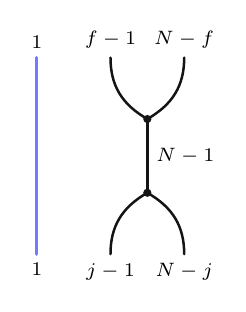
\begin{tikzpicture}[scale=.78,every node/.style={label}]
\draw[marked] (-1.2,0)--(-1.2,3.2);
\draw[a,thickness={j-1}] (0,0)..controls(0,0.45)and(0.18,0.757513)..(0.6,1);
\draw[a,thickness={N-j}] (1.2,0)..controls(1.2,0.45)and(1.02,0.757513)..(0.6,1);
\draw[a,thickness={N-1}] (0.6,1)--(0.6,2.2);
\draw[a,thickness={f-1}] (0.6,2.2)..controls(0.18,2.442487)and(0,2.75)..(0,3.2);
\draw[a,thickness={N-f}] (0.6,2.2)..controls(1.02,2.442487)and(1.2,2.75)..(1.2,3.2);
\node[joint]at(0.6,1){};
\node[joint]at(0.6,2.2){};
\node[inputlabel]at(-1.2,0){$1$};
\node[inputlabel]at(0,0){$j-1$};
\node[inputlabel]at(1.2,0){$N-j$};
\node[outputlabel]at(-1.2,3.2){$1$};
\node[outputlabel]at(0,3.2){$f-1$};
\node[outputlabel]at(1.2,3.2){$N-f$};
\node[edgelabel,right=2pt]at(0.6,1.6){$N-1$};
\end{tikzpicture}}
\newcommand{\StageA}{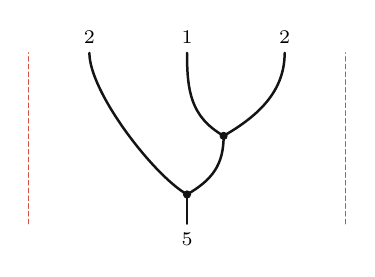
\begin{tikzpicture}[scale=.62]\StageBodyA{5}{2}{1}{4}{3}{3}\end{tikzpicture}}
\newcommand{\PrefixAnnA}{%
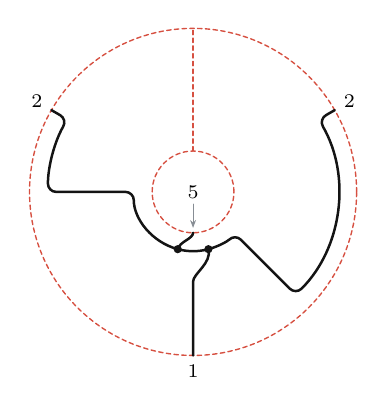
\begin{tikzpicture}[scale=.67]\PrefixAnnBodyA{5}{2}{1}{4}{3}{3}\end{tikzpicture}
}
\newcommand{\StageB}{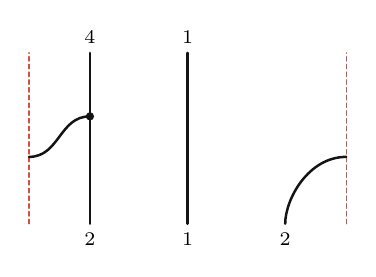
\begin{tikzpicture}[scale=.62]\StageBodyB{5}{2}{1}{4}{3}{3}\end{tikzpicture}}
\newcommand{\PrefixAnnB}{%
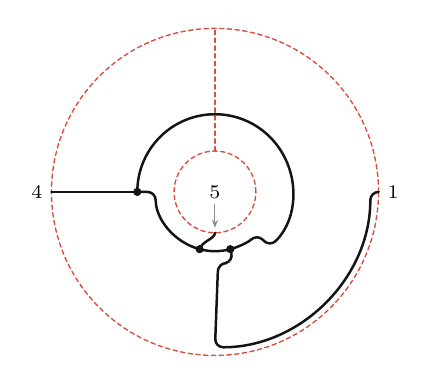
\begin{tikzpicture}[scale=.67]\PrefixAnnBodyB{5}{2}{1}{4}{3}{3}\end{tikzpicture}
}
\newcommand{\StageC}{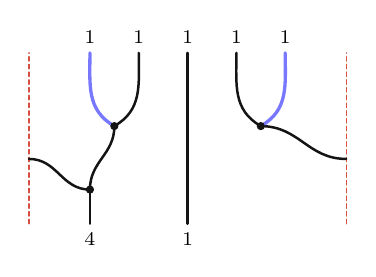
\begin{tikzpicture}[scale=.62]\StageBodyC{5}{2}{1}{4}{3}{3}\end{tikzpicture}}
\newcommand{\PrefixAnnC}{%
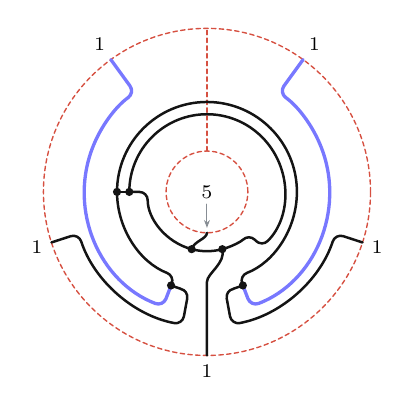
\begin{tikzpicture}[scale=.67]\PrefixAnnBodyC{5}{2}{1}{4}{3}{3}\end{tikzpicture}
}
\newcommand{\StageD}{\begin{tikzpicture}[scale=.62]\StageBodyD{5}{2}{1}{4}{3}{3}\end{tikzpicture}}
\newcommand{\PrefixAnnD}{%
\begin{tikzpicture}[scale=.67]\PrefixAnnBodyD{5}{2}{1}{4}{3}{3}\end{tikzpicture}
}
\newcommand{\StageE}{\begin{tikzpicture}[scale=.62]\StageBodyE{5}{2}{1}{4}{3}{3}\end{tikzpicture}}
\newcommand{\PrefixAnnE}{%
\begin{tikzpicture}[scale=.67]\PrefixAnnBodyE{5}{2}{1}{4}{3}{3}\end{tikzpicture}
}
\newcommand{\StageF}{\begin{tikzpicture}[scale=.62]\StageBodyF{5}{2}{1}{4}{3}{3}\end{tikzpicture}}
\newcommand{\PrefixAnnF}{%
\begin{tikzpicture}[scale=.67]\PrefixAnnBodyF{5}{2}{1}{4}{3}{3}\end{tikzpicture}
}

% Scalar evaluation is the coefficient of the straight strand in these
% ordinary split--merge endomorphisms; it is not a trace or a closure.
\newcommand{\weval}[1]{\left\langle\,#1\,\right\rangle}
\newcommand{\nestedbubble}[5]{\begin{tikzpicture}[scale=.72,every node/.style={label}]
\draw[a,thickness={#5}](0,0)--(0,.5);
\draw[a,thickness={#4}](0,.5)..controls(-.4,.73094)and(-.6,.92)..(-.6,1.2);
\draw[a,thickness={#1}](-.6,1.2)..controls(-1.25,1.57528)and(-1.25,2.42472)..(-.6,2.8);
\draw[a,thickness={#2}](-.6,1.2)..controls(.05,1.57528)and(.05,2.42472)..(-.6,2.8);
\draw[a,thickness={#4}](-.6,2.8)..controls(-.6,3.08)and(-.4,3.26906)..(0,3.5)--(0,4);
\draw[a,thickness={#3}](0,.5)..controls(1.45,1.33716)and(1.45,2.66284)..(0,3.5);
\foreach\x/\y in{0/.5,-.6/1.2,-.6/2.8,0/3.5}\node[joint]at(\x,\y){};
\node[inputlabel]at(0,0){$#5$};\node[outputlabel]at(0,4){$#5$};
\node[edgelabel,left=2pt]at(-1.2,2){$#1$};\node[edgelabel,right=2pt]at(-.1,2){$#2$};\node[edgelabel,right=2pt]at(1.1,2){$#3$};
\node[edgelabel,left=2pt]at(-.62,.88){$#4$};
\end{tikzpicture}}
\newcommand{\nestedbubbleright}[5]{\begin{tikzpicture}[scale=.72,xscale=-1,every node/.style={label}]
\draw[a,thickness={#5}](0,0)--(0,.5);
\draw[a,thickness={#4}](0,.5)..controls(-.4,.73094)and(-.6,.92)..(-.6,1.2);
\draw[a,thickness={#3}](-.6,1.2)..controls(-1.25,1.57528)and(-1.25,2.42472)..(-.6,2.8);
\draw[a,thickness={#2}](-.6,1.2)..controls(.05,1.57528)and(.05,2.42472)..(-.6,2.8);
\draw[a,thickness={#4}](-.6,2.8)..controls(-.6,3.08)and(-.4,3.26906)..(0,3.5)--(0,4);
\draw[a,thickness={#1}](0,.5)..controls(1.45,1.33716)and(1.45,2.66284)..(0,3.5);
\foreach\x/\y in{0/.5,-.6/1.2,-.6/2.8,0/3.5}\node[joint]at(\x,\y){};
\node[inputlabel]at(0,0){$#5$};\node[outputlabel]at(0,4){$#5$};
\node[edgelabel,right=2pt]at(-1.2,2){$#3$};\node[edgelabel,left=2pt]at(-.1,2){$#2$};\node[edgelabel,left=2pt]at(1.1,2){$#1$};
\node[edgelabel,right=2pt]at(-.62,.88){$#4$};
\end{tikzpicture}}
\newcommand{\channelstack}[1]{\begin{tikzpicture}[scale=.78,every node/.style={label}]
\foreach\k in{1,...,#1}{\pgfmathsetmacro{\y}{1.8*(\k-1)}
\draw[a,thickness={1}](-.6,\y)..controls(-.6,\y+.2)and(-.42,\y+.257513)..(0,\y+.5);
\draw[a,thickness={1}](.6,\y)..controls(.6,\y+.2)and(.42,\y+.257513)..(0,\y+.5);
\draw[a](0,\y+.5)--(0,\y+1.3);
\draw[a,thickness={1}](0,\y+1.3)..controls(-.42,\y+1.542487)and(-.6,\y+1.6)..(-.6,\y+1.8);
\draw[a,thickness={1}](0,\y+1.3)..controls(.42,\y+1.542487)and(.6,\y+1.6)..(.6,\y+1.8);
\node[joint]at(0,\y+.5){};\node[joint]at(0,\y+1.3){};
\node[edgelabel,right=2pt]at(0,\y+.9){$2$};}
\foreach\x in{-.6,.6}{\node[inputlabel]at(\x,0){$1$};\node[outputlabel]at(\x,{1.8*#1}){$1$};}
\end{tikzpicture}}
% A word in positive crossings and positive/inverse affine dots. Read upward.
\newcommand{\thinword}[3][0.7]{%
\begin{tikzpicture}[scale=#1,every node/.style={label}]
\foreach\k/\typ[count=\n]in{#3}{\xdef\webwordlength{\n}}
\pgfmathsetmacro{\stepheight}{3/\webwordlength}
\foreach\k/\typ[count=\h from 0]in{#3}{
\pgfmathsetmacro{\y}{\h*\stepheight}\pgfmathsetmacro{\x}{1.1*(\k-1)}
\ifdefstring{\typ}{H}{
\foreach\j in{1,...,#2}{\ifnum\j=\k\else\ifnum\j=\numexpr\k+1\relax\else
\draw[a,thickness={1}]({1.1*(\j-1)},\y)--({1.1*(\j-1)},\y+\stepheight);\fi\fi}
\draw[a,thickness={1}](\x+1.1,\y)to[out=90,in=-90](\x,\y+\stepheight);
\draw[a,over,thickness={1}](\x,\y)to[out=90,in=-90](\x+1.1,\y+\stepheight);
}{
\foreach\j in{1,...,#2}\draw[a,thickness={1}]({1.1*(\j-1)},\y)--({1.1*(\j-1)},\y+\stepheight);
\ifdefstring{\typ}{X}{\def\sgn{+}}{\def\sgn{-}}
\node[affinedot]at(\x,\y+\stepheight/2){$\sgn$};
}}
\foreach\j in{1,...,#2}{
\node[below]at({1.1*(\j-1)},0){$1$};
\node[above]at({1.1*(\j-1)},3){$1$};}
\end{tikzpicture}
}
\newcommand{\splitthreeleft}[5]{\begin{tikzpicture}[scale=.78,every node/.style={label}]
\draw[a,thickness={#5}] (0,0)--(0,0.5);
\draw[a,thickness={#3}] (0,0.5)..controls(0.6,0.84641)and(1.1,1.3)..(1.1,2.4);
\draw[a,thickness={#4}] (0,0.5)..controls(-0.42,0.742487)and(-0.55,0.95)..(-0.55,1.3);
\draw[a,thickness={#2}] (-0.55,1.3)..controls(-0.13,1.542487)and(0,1.8)..(0,2.4);
\draw[a,thickness={#1}] (-0.55,1.3)..controls(-0.97,1.542487)and(-1.1,1.8)..(-1.1,2.4);
\node[joint]at(0,0.5){};
\node[joint]at(-0.55,1.3){};
\node[outputlabel]at(-1.1,2.4){$#1$};
\node[outputlabel]at(0,2.4){$#2$};
\node[outputlabel]at(1.1,2.4){$#3$};
\node[inputlabel]at(0,0){$#5$};
\node[edgelabel,left=2pt]at(-0.57,0.86){$#4$};
\end{tikzpicture}}
\newcommand{\splitthreeright}[5]{\begin{tikzpicture}[scale=.78,every node/.style={label}]
\draw[a,thickness={#5}] (0,0)--(0,0.5);
\draw[a,thickness={#1}] (0,0.5)..controls(-0.6,0.84641)and(-1.1,1.3)..(-1.1,2.4);
\draw[a,thickness={#4}] (0,0.5)..controls(0.42,0.742487)and(0.55,0.95)..(0.55,1.3);
\draw[a,thickness={#2}] (0.55,1.3)..controls(0.13,1.542487)and(0,1.8)..(0,2.4);
\draw[a,thickness={#3}] (0.55,1.3)..controls(0.97,1.542487)and(1.1,1.8)..(1.1,2.4);
\node[joint]at(0,0.5){};
\node[joint]at(0.55,1.3){};
\node[outputlabel]at(-1.1,2.4){$#1$};
\node[outputlabel]at(0,2.4){$#2$};
\node[outputlabel]at(1.1,2.4){$#3$};
\node[inputlabel]at(0,0){$#5$};
\node[edgelabel,right=2pt]at(0.57,0.86){$#4$};
\end{tikzpicture}}
\newcommand{\OneStrongAtS}[1][.4]{\begin{tikzpicture}[scale=#1,yscale=.84]\Ebody{N}{s}{N-s}{s-1}{m}{m-1}{m+1}{right}{m}\end{tikzpicture}}
\newcommand{\OneWeakAtS}[1][.4]{\begin{tikzpicture}[scale=#1,yscale=.84]\Ebody{N}{s}{N-s}{s-1}{m+1}{m}{m}{left}{m}\end{tikzpicture}}
\newcommand{\Bthree}[1][.85]{\begin{tikzpicture}[scale=#1,every node/.style={font=\scriptsize}]
\threebody{7}{3}{4}{3}\end{tikzpicture}}
\newcommand{\VsOneThreeRefined}[1][.58]{\begin{tikzpicture}[scale=#1,yscale=.84]
\WideVrefbody{7}{1}{6}\begin{scope}[yshift=5.6cm]\threebody{\vphantom N}{3}{4}{3}\end{scope}\end{tikzpicture}}

% Thin words are listed in the order read from bottom to top.
\newcommand{\AffineWord}[3]{\begin{tikzpicture}[scale=.78,every node/.style={label}]
\foreach\i/\op[count=\k]in{#2}{
\pgfmathsetmacro{\xx}{1.1*(\i-1)}
\pgfmathsetmacro{\yy}{.9*(\k-1)}
\ifboolexpr{test{\ifdefstring{\op}{H}} or test{\ifdefstring{\op}{h}}}{
\foreach\j in{1,...,#1}{\ifnum\j=\i\else
\pgfmathtruncatemacro{\nexti}{\i+1}\ifnum\j=\nexti\else
\draw[a,thickness={1}]({1.1*(\j-1)},\yy)--({1.1*(\j-1)},\yy+.9);\fi\fi}
\ifdefstring{\op}{H}{
\draw[a,thickness={1}](\xx+1.1,\yy)to[out=90,in=-90](\xx,\yy+.9);
\draw[a,over,thickness={1}](\xx,\yy)to[out=90,in=-90](\xx+1.1,\yy+.9);
}{
\draw[a,thickness={1}](\xx,\yy)to[out=90,in=-90](\xx+1.1,\yy+.9);
\draw[a,over,thickness={1}](\xx+1.1,\yy)to[out=90,in=-90](\xx,\yy+.9);
}
}{
\foreach\j in{1,...,#1}\draw[a,thickness={1}]({1.1*(\j-1)},\yy)--({1.1*(\j-1)},\yy+.9);
\ifdefstring{\op}{X}{\def\dotsign{+}}{\def\dotsign{-}}
\node[affinedot]at(\xx,\yy+.45){$\dotsign$};
}
}
\foreach\j in{1,...,#1}{
\node[below]at({1.1*(\j-1)},0){$1$};
\node[above]at({1.1*(\j-1)},{.9*#3}){$1$};
}
\end{tikzpicture}}

\newcommand{\SpectatorDigon}{\begin{tikzpicture}[scale=.78,every node/.style={label}]
\draw[marked] (-1.8,0)--(-1.8,2.4);
\node[inputlabel]at(-1.8,0){$1$};
\node[outputlabel]at(-1.8,2.4){$1$};
\draw[marked] (1.8,0)--(1.8,2.4);
\node[inputlabel]at(1.8,0){$1$};
\node[outputlabel]at(1.8,2.4){$1$};
\draw[a,thickness={a+b}] (0,0)--(0,0.5);
\draw[a,thickness={a}] (0,0.5)..controls(-0.42,0.742487)and(-0.6,1)..(-0.6,1.2)..controls(-0.6,1.4)and(-0.42,1.657513)..(0,1.9);
\draw[a,thickness={b}] (0,0.5)..controls(0.42,0.742487)and(0.6,1)..(0.6,1.2)..controls(0.6,1.4)and(0.42,1.657513)..(0,1.9);
\draw[a,thickness={a+b}] (0,1.9)--(0,2.4);
\node[joint]at(0,0.5){};
\node[joint]at(0,1.9){};
\node[edgelabel,left=2pt]at(-0.6,1.2){$a$};
\node[edgelabel,right=2pt]at(0.6,1.2){$b$};
\node[inputlabel]at(0,0){$a+b$};
\node[outputlabel]at(0,2.4){$a+b$};
\end{tikzpicture}}
\newcommand{\SpectatorIdentity}{\begin{tikzpicture}[scale=.78,every node/.style={label}]
\draw[marked] (-1.8,0)--(-1.8,2.4);
\node[inputlabel]at(-1.8,0){$1$};
\node[outputlabel]at(-1.8,2.4){$1$};
\draw[marked] (1.8,0)--(1.8,2.4);
\node[inputlabel]at(1.8,0){$1$};
\node[outputlabel]at(1.8,2.4){$1$};
\draw[a,thickness={a+b}] (0,0)--(0,2.4);
\node[inputlabel]at(0,0){$a+b$};
\node[outputlabel]at(0,2.4){$a+b$};
\end{tikzpicture}}

\newcommand{\DottedDigon}[1]{\begin{tikzpicture}[scale=.78,every node/.style={label}]
\draw[a] (0,0)--(0,0.5);
\draw[a,thickness={1}] (0,0.5)..controls(-0.42,0.742487)and(-0.6,1)..(-0.6,1.2)..controls(-0.6,1.4)and(-0.42,1.657513)..(0,1.9);
\draw[a,thickness={1}] (0,0.5)..controls(0.42,0.742487)and(0.6,1)..(0.6,1.2)..controls(0.6,1.4)and(0.42,1.657513)..(0,1.9);
\draw[a] (0,1.9)--(0,2.4);
\node[joint]at(0,0.5){};
\node[joint]at(0,1.9){};
\node[edgelabel,left=2pt]at(-0.6,.82){$1$};
\node[edgelabel,right=2pt]at(0.6,.82){$1$};
\node[inputlabel]at(0,0){$2$};
\node[outputlabel]at(0,2.4){$2$};
\node[affinedot]at(-0.6,1.2){$#1$};
\node[affinedot]at(0.6,1.2){$#1$};
\end{tikzpicture}}
\newcommand{\DeterminantDot}[1]{\begin{tikzpicture}[scale=.78,every node/.style={label}]
\draw[a] (0,0)--(0,2.4);
\node[affinedot]at(0,1.2){$#1$};
\node[inputlabel]at(0,0){$2$};
\node[outputlabel]at(0,2.4){$2$};
\end{tikzpicture}}

% The two retained unit strands frame the middle operation.
\newcommand{\MiddleMerge}{\begin{tikzpicture}[scale=.78,every node/.style={label}]
\draw[marked] (-2.2,0)--(-2.2,2.4);
\node[inputlabel]at(-2.2,0){$1$};
\node[outputlabel]at(-2.2,2.4){$1$};
\draw[marked] (2.2,0)--(2.2,2.4);
\node[inputlabel]at(2.2,0){$1$};
\node[outputlabel]at(2.2,2.4){$1$};
\draw[a,thickness={2*a+1}] (0,1.9)--(0,2.4);
\draw[a,thickness={a}] (1.1,0)..controls(1.1,1.1)and(0.6,1.55359)..(0,1.9);
\draw[a,thickness={a+1}] (-0.55,1.1)..controls(-0.55,1.45)and(-0.42,1.657513)..(0,1.9);
\draw[a,thickness={1}] (0,0)..controls(0,0.6)and(-0.13,0.857513)..(-0.55,1.1);
\draw[a,thickness={a}] (-1.1,0)..controls(-1.1,0.6)and(-0.97,0.857513)..(-0.55,1.1);
\node[joint]at(0,1.9){};
\node[joint]at(-0.55,1.1){};
\node[inputlabel]at(-1.1,0){$a$};
\node[inputlabel]at(0,0){$1$};
\node[inputlabel]at(1.1,0){$a$};
\node[outputlabel]at(0,2.4){$2a+1$};
\end{tikzpicture}}
\newcommand{\MiddleSplit}{\begin{tikzpicture}[scale=.78,every node/.style={label}]
\draw[marked] (-2.2,0)--(-2.2,2.4);
\node[inputlabel]at(-2.2,0){$1$};
\node[outputlabel]at(-2.2,2.4){$1$};
\draw[marked] (2.2,0)--(2.2,2.4);
\node[inputlabel]at(2.2,0){$1$};
\node[outputlabel]at(2.2,2.4){$1$};
\draw[a,thickness={2*a+1}] (0,0)--(0,0.5);
\draw[a,thickness={a}] (0,0.5)..controls(-0.6,0.84641)and(-1.1,1.3)..(-1.1,2.4);
\draw[a,thickness={a+1}] (0,0.5)..controls(0.42,0.742487)and(0.55,0.95)..(0.55,1.3);
\draw[a,thickness={1}] (0.55,1.3)..controls(0.13,1.542487)and(0,1.8)..(0,2.4);
\draw[a,thickness={a}] (0.55,1.3)..controls(0.97,1.542487)and(1.1,1.8)..(1.1,2.4);
\node[joint]at(0,0.5){};
\node[joint]at(0.55,1.3){};
\node[outputlabel]at(-1.1,2.4){$a$};
\node[outputlabel]at(0,2.4){$1$};
\node[outputlabel]at(1.1,2.4){$a$};
\node[inputlabel]at(0,0){$2a+1$};
\end{tikzpicture}}
\newcommand{\MiddleChannel}{\begin{tikzpicture}[scale=.76,every node/.style={label}]
\draw[marked] (-2.2,0)--(-2.2,4.8);
\node[inputlabel]at(-2.2,0){$1$};
\node[outputlabel]at(-2.2,4.8){$1$};
\draw[marked] (2.2,0)--(2.2,4.8);
\node[inputlabel]at(2.2,0){$1$};
\node[outputlabel]at(2.2,4.8){$1$};
\draw[a,thickness={2*a+1}] (0,1.9)--(0,2.4);
\draw[a,thickness={a}] (1.1,0)..controls(1.1,1.1)and(0.6,1.55359)..(0,1.9);
\draw[a,thickness={a+1}] (-0.55,1.1)..controls(-0.55,1.45)and(-0.42,1.657513)..(0,1.9);
\draw[a,thickness={1}] (0,0)..controls(0,0.6)and(-0.13,0.857513)..(-0.55,1.1);
\draw[a,thickness={a}] (-1.1,0)..controls(-1.1,0.6)and(-0.97,0.857513)..(-0.55,1.1);
\node[joint]at(0,1.9){};
\node[joint]at(-0.55,1.1){};
\draw[a,thickness={2*a+1}] (0,2.4)--(0,2.9);
\draw[a,thickness={a}] (0,2.9)..controls(-0.6,3.24641)and(-1.1,3.7)..(-1.1,4.8);
\draw[a,thickness={a+1}] (0,2.9)..controls(0.42,3.142487)and(0.55,3.35)..(0.55,3.7);
\draw[a,thickness={1}] (0.55,3.7)..controls(0.13,3.942487)and(0,4.2)..(0,4.8);
\draw[a,thickness={a}] (0.55,3.7)..controls(0.97,3.942487)and(1.1,4.2)..(1.1,4.8);
\node[joint]at(0,2.9){};
\node[joint]at(0.55,3.7){};
\node[inputlabel]at(-1.1,0){$a$};
\node[inputlabel]at(0,0){$1$};
\node[inputlabel]at(1.1,0){$a$};
\node[outputlabel]at(-1.1,4.8){$a$};
\node[outputlabel]at(0,4.8){$1$};
\node[outputlabel]at(1.1,4.8){$a$};
\node[edgelabel,right=2pt]at(0,2.4){$2a+1$};
\end{tikzpicture}}

\newcommand{\RefineThreeStrong}{\begin{tikzpicture}[scale=.78,every node/.style={label}]
\draw[a,directed] (-1.1,0)--(-1.1,1.8);
\draw[a] (0.55,0)--(0.55,0.5);
\draw[a,thickness={1}] (0.55,0.5)..controls(0.13,0.742487)and(0,1.1)..(0,1.8);
\draw[a,directed] (0.55,0.5)..controls(0.97,0.742487)and(1.1,1.1)..(1.1,1.8);
\node[joint]at(0.55,0.5){};
\node[outputlabel]at(-1.1,1.8){$3$};
\node[outputlabel]at(0,1.8){$1$};
\node[outputlabel]at(1.1,1.8){$3$};
\node[inputlabel]at(-1.1,0){$3$};
\node[inputlabel]at(0.55,0){$4$};
\end{tikzpicture}}
\newcommand{\RefineThreeWeak}{\begin{tikzpicture}[scale=.78,every node/.style={label}]
\draw[a,directed] (1.1,0)--(1.1,1.8);
\draw[a] (-0.55,0)--(-0.55,0.5);
\draw[a,thickness={1}] (-0.55,0.5)..controls(-0.13,0.742487)and(0,1.1)..(0,1.8);
\draw[a,directed] (-0.55,0.5)..controls(-0.97,0.742487)and(-1.1,1.1)..(-1.1,1.8);
\node[joint]at(-0.55,0.5){};
\node[outputlabel]at(-1.1,1.8){$3$};
\node[outputlabel]at(0,1.8){$1$};
\node[outputlabel]at(1.1,1.8){$3$};
\node[inputlabel]at(1.1,0){$3$};
\node[inputlabel]at(-0.55,0){$4$};
\end{tikzpicture}}

\newcommand{\Rfour}[1][.44]{\begin{tikzpicture}[scale=#1,yscale=.84]
\WideRbody{9}{4}{3}{8}{7}{5}\end{tikzpicture}}
\newcommand{\Bfour}{\begin{tikzpicture}[scale=.66]
\threebody{9}{4}{5}{4}\end{tikzpicture}}

\newcommand{\CompositionStrip}[1][0.85]{\begin{tikzpicture}[scale=#1,every node/.style={label}]
\draw[gluing](-1.2,1.2)--(1.2,1.2);
\draw[a,thickness={1}] (-0.6,0)..controls(-0.6,0.25)and(-0.42,0.407513)..(0,0.65);
\draw[a] (0.6,0)..controls(0.6,0.25)and(0.42,0.407513)..(0,0.65);
\draw[a] (0,0.65)--(0,1.75);
\draw[a,thickness={1}] (0,1.75)..controls(-0.42,1.992487)and(-0.6,2.15)..(-0.6,2.4);
\draw[a] (0,1.75)..controls(0.42,1.992487)and(0.6,2.15)..(0.6,2.4);
\node[joint]at(0,0.65){};
\node[joint]at(0,1.75){};
\node[edgelabel,right=2pt]at(0,1.2){$3$};
\node[inputlabel]at(-0.6,0){$1$};
\node[inputlabel]at(0.6,0){$2$};
\node[outputlabel]at(-0.6,2.4){$1$};
\node[outputlabel]at(0.6,2.4){$2$};
\end{tikzpicture}}

\newcommand{\CompositionAnnulus}[1][0.85]{\begin{tikzpicture}[scale=#1,every node/.style={label}]
\begin{scope}[scale=0.65]
\draw[rim](0,0)circle(1) (0,0)circle(4);
\draw[cut](90:1)--(90:4);
\draw[gluing](0,0)circle(2.5);
\draw[a,rounded corners=3pt,thickness={1}] (-180:1)--(-180:1.8) arc[start angle=-180,end angle=-90,radius=1.8];
\draw[a,rounded corners=3pt] (0:1)--(0:1.8) arc[start angle=0,end angle=-90,radius=1.8];
\draw[a,rounded corners=3pt] (-90:1.8)--(-90:3.2);
\draw[a,rounded corners=3pt,thickness={1}] (-90:3.2) arc[start angle=-90,end angle=-180,radius=3.2]--(-180:4);
\draw[a,rounded corners=3pt] (-90:3.2) arc[start angle=-90,end angle=0,radius=3.2]--(0:4);
\node[joint]at(-90:1.8){};
\node[joint]at(-90:3.2){};
\annularinputlabel{-180}{1}{1}
\annularinputlabel{0}{1}{2}
\annularlabel{-180}{4}{1}
\annularlabel{0}{4}{2}
\node[edgelabel,right=2pt]at(0,-2.5){$3$};
\end{scope}
\end{tikzpicture}}

\newcommand{\RotationPositiveStrip}[1][0.85]{%
\begin{tikzpicture}[scale=#1]
\draw[cut] (-2,0)--(-2,2.6) (2,0)--(2,2.6);
\draw[a,thickness={1}] (-1,0)..controls(-1,0.85)and(0,1.75)..(0,2.6);
\draw[a,thickness={1}] (0,0)..controls(0,0.85)and(1,1.75)..(1,2.6);
\draw[a,thickness={1}] (1,0)--(1,0.45)..controls(1,0.85)and(1.5,1.3)..(2,1.3);
\draw[a,thickness={1}] (-2,1.3)..controls(-1.5,1.3)and(-1,1.75)..(-1,2.15)--(-1,2.6);
\node[inputlabel]at(-1,0){$1$};
\node[inputlabel]at(0,0){$1$};
\node[inputlabel]at(1,0){$1$};
\node[outputlabel]at(-1,2.6){$1$};
\node[outputlabel]at(0,2.6){$1$};
\node[outputlabel]at(1,2.6){$1$};
\ifwebdetails
\fi
\ifwebdetails
\node[seamlabel,anchor=east]at(-2.117647,1.47){$\alpha$};
\node[seamlabel,anchor=west]at(2.117647,1.47){$\alpha$};
\fi
\end{tikzpicture}
}

\newcommand{\RotationPositiveAnnulus}[1][0.78]{\begin{tikzpicture}[scale=#1,every node/.style={label}]
\begin{scope}[scale=0.55]
\draw[rim](0,0)circle(1) (0,0)circle(4);
\draw[cut](90:1)--(90:4);
\draw[a,thickness={1}]plot[domain=0:1,samples=151,variable=\t] ({-210+(120)*\t*\t*(3-2*\t)}:{1+3*\t});
\draw[a,thickness={1}]plot[domain=0:1,samples=151,variable=\t] ({-90+(120)*\t*\t*(3-2*\t)}:{1+3*\t});
\draw[a,thickness={1}]plot[domain=0:1,samples=151,variable=\t] ({30+(120)*\t*\t*(3-2*\t)}:{1+3*\t});
\annularinputlabel{-210}{1}{1}
\annularlabel{-90}{4}{1}
\annularinputlabel{-90}{1}{1}
\annularlabel{30}{4}{1}
\annularinputlabel{30}{1}{1}
\annularlabel{150}{4}{1}
\end{scope}
\end{tikzpicture}}

\newcommand{\RotationNegativeStrip}[1][0.85]{%
\begin{tikzpicture}[scale=#1]
\draw[cut] (-2,0)--(-2,2.6) (2,0)--(2,2.6);
\draw[a,thickness={1}] (1,0)..controls(1,0.85)and(0,1.75)..(0,2.6);
\draw[a,thickness={1}] (0,0)..controls(0,0.85)and(-1,1.75)..(-1,2.6);
\draw[a,thickness={1}] (-1,0)--(-1,0.45)..controls(-1,0.85)and(-1.5,1.3)..(-2,1.3);
\draw[a,thickness={1}] (2,1.3)..controls(1.5,1.3)and(1,1.75)..(1,2.15)--(1,2.6);
\node[inputlabel]at(-1,0){$1$};
\node[inputlabel]at(0,0){$1$};
\node[inputlabel]at(1,0){$1$};
\node[outputlabel]at(-1,2.6){$1$};
\node[outputlabel]at(0,2.6){$1$};
\node[outputlabel]at(1,2.6){$1$};
\ifwebdetails
\fi
\ifwebdetails
\node[seamlabel,anchor=east]at(-2.117647,1.47){$\alpha$};
\node[seamlabel,anchor=west]at(2.117647,1.47){$\alpha$};
\fi
\end{tikzpicture}
}

\newcommand{\RotationNegativeAnnulus}[1][0.78]{\begin{tikzpicture}[scale=#1,every node/.style={label}]
\begin{scope}[scale=0.55]
\draw[rim](0,0)circle(1) (0,0)circle(4);
\draw[cut](90:1)--(90:4);
\draw[a,thickness={1}]plot[domain=0:1,samples=151,variable=\t] ({-210+(-120)*\t*\t*(3-2*\t)}:{1+3*\t});
\draw[a,thickness={1}]plot[domain=0:1,samples=151,variable=\t] ({-90+(-120)*\t*\t*(3-2*\t)}:{1+3*\t});
\draw[a,thickness={1}]plot[domain=0:1,samples=151,variable=\t] ({30+(-120)*\t*\t*(3-2*\t)}:{1+3*\t});
\annularinputlabel{-210}{1}{1}
\annularlabel{-330}{4}{1}
\annularinputlabel{-90}{1}{1}
\annularlabel{-210}{4}{1}
\annularinputlabel{30}{1}{1}
\annularlabel{-90}{4}{1}
\end{scope}
\end{tikzpicture}}

\newcommand{\SphericalStageOne}[1][0.86]{%
\begin{tikzpicture}[scale=#1]
\begin{scope}[scale=0.6625]
\draw[rim](0,0)circle(1) (0,0)circle(4);
\draw[cut](90:1)--(90:4);
\draw[a,rounded corners=3pt] (-90:1)--(-90:1.25);
\draw[a,rounded corners=3pt] (-90:1.25) arc[start angle=-90,end angle=-180,radius=1.25]--(-180:4);
\draw[a,rounded corners=3pt] (-90:1.25) arc[start angle=-90,end angle=0,radius=1.25]--(0:4);
\node[joint]at(-90:1.25){};
\node[boundarylabel]at(0,0){$5$};
\annularlabel{-180}{4}{2}
\annularlabel{0}{4}{3}
\draw[draw=webguide,-{Stealth[length=1mm]},line width=.35pt](0,-.3)--(0,-.88);
\end{scope}
\end{tikzpicture}
}

\newcommand{\SphericalStageTwo}[1][0.86]{%
\begin{tikzpicture}[scale=#1]
\begin{scope}[scale=0.6625]
\draw[rim](0,0)circle(1) (0,0)circle(4);
\draw[cut](90:1)--(90:4);
\draw[a,rounded corners=3pt] (-90:1)--(-90:1.25);
\draw[a,rounded corners=3pt] (-90:1.25) arc[start angle=-90,end angle=-180,radius=1.25]--(-180:1.9);
\draw[a,rounded corners=3pt] (-90:1.25)--(-90:1.9) arc[start angle=-90,end angle=180,radius=1.9];
\draw[a,rounded corners=3pt] (-180:1.9)--(-180:3.55) arc[start angle=-180,end angle=-90,radius=3.55]--(-90:4);
\node[joint]at(-90:1.25){};
\node[joint]at(-180:1.9){};
\node[boundarylabel]at(0,0){$5$};
\annularlabel{-90}{4}{5}
\draw[draw=webguide,-{Stealth[length=1mm]},line width=.35pt](0,-.3)--(0,-.88);
\end{scope}
\end{tikzpicture}
}

\newcommand{\SphericalStageThree}[1][0.86]{%
\begin{tikzpicture}[scale=#1]
\begin{scope}[scale=0.6625]
\draw[rim](0,0)circle(1) (0,0)circle(4);
\draw[cut](90:1)--(90:4);
\draw[a,rounded corners=3pt] (-90:1)--(-90:1.25);
\draw[a,rounded corners=3pt] (-90:1.25) arc[start angle=-90,end angle=-180,radius=1.25]--(-180:1.9);
\draw[a,rounded corners=3pt] (-90:1.25)--(-90:1.9) arc[start angle=-90,end angle=180,radius=1.9];
\draw[a,rounded corners=3pt] (-180:1.9)--(-180:2.2);
\draw[a,rounded corners=3pt] (-180:2.2)--(-180:4);
\draw[a,rounded corners=3pt] (-180:2.2) arc[start angle=-180,end angle=-360,radius=2.2]--(0:4);
\node[joint]at(-90:1.25){};
\node[joint]at(-180:1.9){};
\node[joint]at(-180:2.2){};
\node[boundarylabel]at(0,0){$5$};
\annularlabel{-180}{4}{2}
\annularlabel{0}{4}{3}
\draw[draw=webguide,-{Stealth[length=1mm]},line width=.35pt](0,-.3)--(0,-.88);
\end{scope}
\end{tikzpicture}
}

\newcommand{\SphericalStageFour}[1][0.86]{%
\begin{tikzpicture}[scale=#1]
\begin{scope}[scale=0.6625]
\draw[rim](0,0)circle(1) (0,0)circle(4);
\draw[cut](90:1)--(90:4);
\draw[a,rounded corners=3pt] (-90:1)--(-90:1.25);
\draw[a,rounded corners=3pt] (-90:1.25) arc[start angle=-90,end angle=-180,radius=1.25]--(-180:1.9);
\draw[a,rounded corners=3pt] (-90:1.25)--(-90:1.9) arc[start angle=-90,end angle=180,radius=1.9];
\draw[a,rounded corners=3pt] (-180:1.9)--(-180:2.2);
\draw[a,rounded corners=3pt] (-180:2.2)--(-180:3.55) arc[start angle=-180,end angle=-90,radius=3.55];
\draw[a,rounded corners=3pt] (-180:2.2) arc[start angle=-180,end angle=-450,radius=2.2]--(-90:3.55);
\draw[a,rounded corners=3pt] (-90:3.55)--(-90:4);
\node[joint]at(-90:1.25){};
\node[joint]at(-180:1.9){};
\node[joint]at(-180:2.2){};
\node[joint]at(-90:3.55){};
\node[boundarylabel]at(0,0){$5$};
\annularlabel{-90}{4}{5}
\draw[draw=webguide,-{Stealth[length=1mm]},line width=.35pt](0,-.3)--(0,-.88);
\end{scope}
\end{tikzpicture}
}

\newcommand{\SphericalAnnFiveOne}[1][0.78]{%
\begin{tikzpicture}[scale=#1]
\begin{scope}[scale=0.6625]
\draw[rim](0,0)circle(1) (0,0)circle(4);
\draw[cut](90:1)--(90:4);
\draw[a,rounded corners=3pt] (-90:1)--(-90:1.25);
\draw[a,rounded corners=3pt,thickness={1}] (-90:1.25) arc[start angle=-90,end angle=-180,radius=1.25]--(-180:1.9);
\draw[a,rounded corners=3pt] (-90:1.25)--(-90:1.9) arc[start angle=-90,end angle=180,radius=1.9];
\draw[a,rounded corners=3pt] (-180:1.9)--(-180:2.2);
\draw[a,rounded corners=3pt,thickness={1}] (-180:2.2)--(-180:3.55) arc[start angle=-180,end angle=-90,radius=3.55];
\draw[a,rounded corners=3pt] (-180:2.2) arc[start angle=-180,end angle=-450,radius=2.2]--(-90:3.55);
\draw[a,rounded corners=3pt] (-90:3.55)--(-90:4);
\node[joint]at(-90:1.25){};
\node[joint]at(-180:1.9){};
\node[joint]at(-180:2.2){};
\node[joint]at(-90:3.55){};
\node[boundarylabel]at(0,0){$5$};
\annularlabel{-90}{4}{5}
\draw[draw=webguide,-{Stealth[length=1mm]},line width=.35pt](0,-.3)--(0,-.88);
\end{scope}
\end{tikzpicture}
}

\newcommand{\SphericalAnnFiveTwo}[1][0.78]{%
\begin{tikzpicture}[scale=#1]
\begin{scope}[scale=0.6625]
\draw[rim](0,0)circle(1) (0,0)circle(4);
\draw[cut](90:1)--(90:4);
\draw[a,rounded corners=3pt] (-90:1)--(-90:1.25);
\draw[a,rounded corners=3pt] (-90:1.25) arc[start angle=-90,end angle=-180,radius=1.25]--(-180:1.9);
\draw[a,rounded corners=3pt] (-90:1.25)--(-90:1.9) arc[start angle=-90,end angle=180,radius=1.9];
\draw[a,rounded corners=3pt] (-180:1.9)--(-180:2.2);
\draw[a,rounded corners=3pt] (-180:2.2)--(-180:3.55) arc[start angle=-180,end angle=-90,radius=3.55];
\draw[a,rounded corners=3pt] (-180:2.2) arc[start angle=-180,end angle=-450,radius=2.2]--(-90:3.55);
\draw[a,rounded corners=3pt] (-90:3.55)--(-90:4);
\node[joint]at(-90:1.25){};
\node[joint]at(-180:1.9){};
\node[joint]at(-180:2.2){};
\node[joint]at(-90:3.55){};
\node[boundarylabel]at(0,0){$5$};
\annularlabel{-90}{4}{5}
\draw[draw=webguide,-{Stealth[length=1mm]},line width=.35pt](0,-.3)--(0,-.88);
\end{scope}
\end{tikzpicture}
}

\newcommand{\IdentityAnnFive}[1][0.78]{%
\begin{tikzpicture}[scale=#1]
\begin{scope}[scale=.6625]
\draw[rim](0,0)circle(1) (0,0)circle(4);
\draw[cut](90:1)--(90:4);
\draw[a](0,-1)--(0,-4);
\node[boundarylabel]at(0,0){$5$};
\draw[draw=webguide,-{Stealth[length=1mm]},line width=.35pt](0,-.3)--(0,-.88);
\annularlabel{-90}{4}{5}
\node[edgelabel,above=2pt]at(0,4){$\text{identity}$};
\end{scope}
\end{tikzpicture}
}

\newcommand{\OneLineStageOne}[1][0.86]{%
\begin{tikzpicture}[scale=#1]
\begin{scope}[scale=0.6625]
\draw[rim](0,0)circle(1) (0,0)circle(4);
\draw[cut](90:1)--(90:4);
\draw[a,rounded corners=3pt] (-90:1)--(-90:1.25);
\draw[a,rounded corners=3pt] (-90:1.25) arc[start angle=-90,end angle=-180,radius=1.25]--(-180:4);
\draw[a,rounded corners=3pt] (-90:1.25) arc[start angle=-90,end angle=0,radius=1.25]--(0:4);
\node[joint]at(-90:1.25){};
\node[boundarylabel]at(0,0){$7$};
\annularlabel{-180}{4}{2}
\annularlabel{0}{4}{5}
\draw[draw=webguide,-{Stealth[length=1mm]},line width=.35pt](0,-.3)--(0,-.88);
\end{scope}
\end{tikzpicture}
}

\newcommand{\OneLineStageTwo}[1][0.86]{%
\begin{tikzpicture}[scale=#1]
\begin{scope}[scale=0.6625]
\draw[rim](0,0)circle(1) (0,0)circle(4);
\draw[cut](90:1)--(90:4);
\draw[a,rounded corners=3pt] (-90:1)--(-90:1.25);
\draw[a,rounded corners=3pt] (-90:1.25) arc[start angle=-90,end angle=-180,radius=1.25]--(-180:1.9);
\draw[a,rounded corners=3pt] (-90:1.25)--(-90:1.9) arc[start angle=-90,end angle=180,radius=1.9];
\draw[a,rounded corners=3pt] (-180:1.9)--(-180:3.55) arc[start angle=-180,end angle=-90,radius=3.55]--(-90:4);
\node[joint]at(-90:1.25){};
\node[joint]at(-180:1.9){};
\node[boundarylabel]at(0,0){$7$};
\annularlabel{-90}{4}{7}
\draw[draw=webguide,-{Stealth[length=1mm]},line width=.35pt](0,-.3)--(0,-.88);
\end{scope}
\end{tikzpicture}
}

\newcommand{\OneLineStageThree}[1][0.86]{%
\begin{tikzpicture}[scale=#1]
\begin{scope}[scale=0.6625]
\draw[rim](0,0)circle(1) (0,0)circle(4);
\draw[cut](90:1)--(90:4);
\draw[a,rounded corners=3pt] (-90:1)--(-90:1.25);
\draw[a,rounded corners=3pt] (-90:1.25) arc[start angle=-90,end angle=-180,radius=1.25]--(-180:1.9);
\draw[a,rounded corners=3pt] (-90:1.25)--(-90:1.9) arc[start angle=-90,end angle=180,radius=1.9];
\draw[a,rounded corners=3pt] (-180:1.9)--(-180:2.2);
\draw[a,rounded corners=3pt] (-180:2.2) arc[start angle=-180,end angle=-100.5,radius=2.2]--(-100.5:2.45);
\draw[a,rounded corners=3pt] (-180:2.2) arc[start angle=-180,end angle=-439.5,radius=2.2]--(-79.5:3.55);
\draw[a,rounded corners=3pt,thickness={1}] (-100.5:2.45) arc[start angle=-100.5,end angle=-90,radius=2.45]--(-90:3.55) arc[start angle=-90,end angle=-79.5,radius=3.55];
\draw[marked,rounded corners=3pt] (-100.5:2.45)--(-100.5:3.55) arc[start angle=-100.5,end angle=-180,radius=3.55]--(-180:4);
\draw[a,rounded corners=3pt] (-79.5:3.55) arc[start angle=-79.5,end angle=0,radius=3.55]--(0:4);
\node[joint]at(-90:1.25){};
\node[joint]at(-180:1.9){};
\node[joint]at(-180:2.2){};
\node[joint]at(-79.5:3.55){};
\node[joint]at(-100.5:2.45){};
\node[boundarylabel]at(0,0){$7$};
\annularlabel{-180}{4}{1}
\annularlabel{0}{4}{6}
\draw[draw=webguide,-{Stealth[length=1mm]},line width=.35pt](0,-.3)--(0,-.88);
\end{scope}
\end{tikzpicture}
}

\newcommand{\OneLineStageFour}[1][0.86]{%
\begin{tikzpicture}[scale=#1]
\begin{scope}[scale=0.6625]
\draw[rim](0,0)circle(1) (0,0)circle(4);
\draw[cut](90:1)--(90:4);
\draw[a,rounded corners=3pt] (-90:1)--(-90:1.25);
\draw[a,rounded corners=3pt] (-90:1.25) arc[start angle=-90,end angle=-180,radius=1.25]--(-180:1.9);
\draw[a,rounded corners=3pt] (-90:1.25)--(-90:1.9) arc[start angle=-90,end angle=180,radius=1.9];
\draw[a,rounded corners=3pt] (-180:1.9)--(-180:2.2);
\draw[a,rounded corners=3pt] (-180:2.2) arc[start angle=-180,end angle=-100.5,radius=2.2]--(-100.5:2.45);
\draw[a,rounded corners=3pt] (-180:2.2) arc[start angle=-180,end angle=-439.5,radius=2.2]--(-79.5:2.45);
\draw[marked,rounded corners=3pt] (-100.5:2.45)--(-100.5:3.55);
\draw[a,rounded corners=3pt,thickness={1}] (-100.5:2.45) arc[start angle=-100.5,end angle=-79.5,radius=2.45];
\draw[a,rounded corners=3pt] (-79.5:2.45)--(-79.5:3.55);
\draw[a,rounded corners=3pt] (-79.5:3.55) arc[start angle=-79.5,end angle=-100.5,radius=3.55];
\draw[a,rounded corners=3pt] (-100.5:3.55) arc[start angle=-100.5,end angle=-180,radius=3.55]--(-180:4);
\draw[a,rounded corners=3pt] (-79.5:3.55) arc[start angle=-79.5,end angle=0,radius=3.55]--(0:4);
\node[joint]at(-90:1.25){};
\node[joint]at(-180:1.9){};
\node[joint]at(-180:2.2){};
\node[joint]at(-100.5:3.55){};
\node[joint]at(-79.5:3.55){};
\node[joint]at(-100.5:2.45){};
\node[joint]at(-79.5:2.45){};
\node[boundarylabel]at(0,0){$7$};
\annularlabel{-180}{4}{3}
\annularlabel{0}{4}{4}
\draw[draw=webguide,-{Stealth[length=1mm]},line width=.35pt](0,-.3)--(0,-.88);
\end{scope}
\end{tikzpicture}
}

\newcommand{\OneLineCoarseStrong}[1][0.4]{%
\begin{tikzpicture}[scale=#1,yscale=.84]
\webcuts{-2.6}{2.6}{7.5}
\draw[a] (0,0)--(0,0.6);
\draw[a] (0,0.6)..controls(-0.433013,0.85)and(-1.2,2.38)..(-1.2,2.8);
\draw[a] (0,0.6)..controls(0.433013,0.85)and(1.6,2.2)..(2.6,2.2);
\draw[a] (-2.6,2.2)..controls(-2,2.2)and(-1.62,2.8)..(-1.2,2.8);
\draw[a] (-1.2,2.8)--(-1.2,3.7);
\draw[a] (-1.2,3.7)..controls(-1.62,3.7)and(-2,4.3)..(-2.6,4.3);
\draw[a] (2.6,4.3)..controls(2,4.3)and(1.2,4.3)..(1.2,5.2);
\draw[a] (-1.2,3.7)..controls(-1.2,4.12)and(-1.2,4.78)..(-1.2,5.2);
\draw[marked] (-1.2,5.2)--(-1.2,6.7);
\draw[a,thickness={1}] (-1.2,5.2)--(1.2,5.2);
\draw[a] (1.2,5.2)--(1.2,6.7);
\draw[a] (1.2,6.7)--(-1.2,6.7);
\draw[a] (1.2,6.7)..controls(1.591918,6.926274)and(2,7.05)..(2,7.5);
\draw[a] (-1.2,6.7)..controls(-1.2,7.152548)and(-2,7.05)..(-2,7.5);
\node[joint]at(0,0.6){};
\node[joint]at(-1.2,2.8){};
\node[joint]at(-1.2,3.7){};
\node[joint]at(1.2,6.7){};
\node[joint]at(-1.2,6.7){};
\node[joint]at(-1.2,5.2){};
\node[joint]at(1.2,5.2){};
\node[inputlabel]at(0,0){$7$};
\node[outputlabel]at(-2,7.5){$3$};
\node[outputlabel]at(2,7.5){$4$};
\ifwebdetails
\node[edgelabel,anchor=east]at(-1.4,1.5){$2$};
\node[edgelabel,anchor=north]at(1.4,1.4){$5$};
\node[edgelabel,anchor=east]at(-1.4,3.2){$7$};
\node[edgelabel,anchor=east]at(-1.4,5.95){$1$};
\node[edgelabel,anchor=east]at(1,4.75){$5$};
\node[edgelabel,anchor=west]at(1.42,5.95){$6$};
\else
\node[edgelabel,anchor=east]at(-1.4,1.5){$2$};
\node[edgelabel,anchor=west,xshift=2pt]at(2.6,1.15){$5$};
\fi
\ifwebdetails
\node[seamlabel,anchor=east]at(-2.7,2.37){$\alpha$};
\node[seamlabel,anchor=west]at(2.7,2.37){$\alpha$};
\node[seamlabel,anchor=east]at(-2.7,4.47){$\beta$};
\node[seamlabel,anchor=west]at(2.7,4.47){$\beta$};
\fi
\end{tikzpicture}
}

\newcommand{\OneLineCoarseWeak}[1][0.4]{%
\begin{tikzpicture}[scale=#1,yscale=.84]
\webcuts{-2.6}{2.6}{7.5}
\draw[a] (0,0)--(0,0.6);
\draw[a] (0,0.6)..controls(-0.433013,0.85)and(-1.2,2.38)..(-1.2,2.8);
\draw[a] (0,0.6)..controls(0.433013,0.85)and(1.6,2.2)..(2.6,2.2);
\draw[a] (-2.6,2.2)..controls(-2,2.2)and(-1.62,2.8)..(-1.2,2.8);
\draw[a] (-1.2,2.8)--(-1.2,3.7);
\draw[a] (-1.2,3.7)..controls(-1.62,3.7)and(-2,4.3)..(-2.6,4.3);
\draw[a] (2.6,4.3)..controls(2,4.3)and(1.2,4.3)..(1.2,5.2);
\draw[a] (-1.2,3.7)..controls(-1.2,4.12)and(-1.2,4.78)..(-1.2,5.2);
\draw[marked] (-1.2,5.2)--(-1.2,6.7);
\draw[a,thickness={1}] (-1.2,5.2)--(1.2,5.2);
\draw[a] (1.2,5.2)--(1.2,6.7);
\draw[a] (1.2,6.7)--(-1.2,6.7);
\draw[a] (1.2,6.7)..controls(1.591918,6.926274)and(2,7.05)..(2,7.5);
\draw[a] (-1.2,6.7)..controls(-1.2,7.152548)and(-2,7.05)..(-2,7.5);
\node[joint]at(0,0.6){};
\node[joint]at(-1.2,2.8){};
\node[joint]at(-1.2,3.7){};
\node[joint]at(1.2,6.7){};
\node[joint]at(-1.2,6.7){};
\node[joint]at(-1.2,5.2){};
\node[joint]at(1.2,5.2){};
\node[inputlabel]at(0,0){$7$};
\node[outputlabel]at(-2,7.5){$4$};
\node[outputlabel]at(2,7.5){$3$};
\ifwebdetails
\node[edgelabel,anchor=east]at(-1.4,1.5){$2$};
\node[edgelabel,anchor=north]at(1.4,1.4){$5$};
\node[edgelabel,anchor=east]at(-1.4,3.2){$7$};
\node[edgelabel,anchor=east]at(-1.4,5.95){$1$};
\node[edgelabel,anchor=east]at(1,4.75){$5$};
\node[edgelabel,anchor=west]at(1.42,5.95){$6$};
\else
\node[edgelabel,anchor=east]at(-1.4,1.5){$2$};
\node[edgelabel,anchor=west,xshift=2pt]at(2.6,1.15){$5$};
\fi
\ifwebdetails
\node[seamlabel,anchor=east]at(-2.7,2.37){$\alpha$};
\node[seamlabel,anchor=west]at(2.7,2.37){$\alpha$};
\node[seamlabel,anchor=east]at(-2.7,4.47){$\beta$};
\node[seamlabel,anchor=west]at(2.7,4.47){$\beta$};
\fi
\end{tikzpicture}
}

\newcommand{\OneLineFineStrong}[1][0.4]{%
\begin{tikzpicture}[scale=#1,yscale=.84]
\webcuts{-2.6}{2.6}{8.8}
\draw[a] (0,0)--(0,0.6);
\draw[a] (0,0.6)..controls(-0.433013,0.85)and(-1.2,2.38)..(-1.2,2.8);
\draw[a] (0,0.6)..controls(0.433013,0.85)and(1.6,2.2)..(2.6,2.2);
\draw[a] (-2.6,2.2)..controls(-2,2.2)and(-1.62,2.8)..(-1.2,2.8);
\draw[a] (-1.2,2.8)--(-1.2,3.7);
\draw[a] (-1.2,3.7)..controls(-1.62,3.7)and(-2,4.3)..(-2.6,4.3);
\draw[a] (2.6,4.3)..controls(2,4.3)and(1.2,4.3)..(1.2,5.2);
\draw[a] (-1.2,3.7)..controls(-1.2,4.12)and(-1.2,4.78)..(-1.2,5.2);
\draw[marked] (-1.2,5.2)--(-1.2,6.7);
\draw[a,thickness={1}] (-1.2,5.2)--(1.2,5.2);
\draw[a] (1.2,5.2)--(1.2,6.7);
\draw[a] (1.2,6.7)--(-1.2,6.7);
\draw[a] (1.2,6.7)--(1.2,7.5);
\draw[a] (-1.2,6.7)--(-1.2,7.5);
\draw[a] (-1.2,7.5)..controls(-1.2,8.1)and(-2,8.35)..(-2,8.8);
\draw[a,thickness={1}] (1.2,7.5)..controls(0.680385,7.8)and(0,8.35)..(0,8.8);
\draw[a] (1.2,7.5)..controls(1.719615,7.8)and(2,8.35)..(2,8.8);
\node[joint]at(0,0.6){};
\node[joint]at(-1.2,2.8){};
\node[joint]at(-1.2,3.7){};
\node[joint]at(1.2,6.7){};
\node[joint]at(-1.2,6.7){};
\node[joint]at(-1.2,5.2){};
\node[joint]at(1.2,5.2){};
\node[joint]at(1.2,7.5){};
\node[inputlabel]at(0,0){$7$};
\node[outputlabel]at(-2,8.8){$3$};
\node[outputlabel]at(0,8.8){$1$};
\node[outputlabel]at(2,8.8){$3$};
\ifwebdetails
\node[edgelabel,anchor=east]at(-1.4,1.5){$2$};
\node[edgelabel,anchor=north]at(1.4,1.4){$5$};
\node[edgelabel,anchor=east]at(-1.4,3.2){$7$};
\node[edgelabel,anchor=east]at(-1.4,5.95){$1$};
\node[edgelabel,anchor=east]at(1,4.75){$5$};
\node[edgelabel,anchor=west]at(1.42,5.95){$6$};
\else
\node[edgelabel,anchor=east]at(-1.4,1.5){$2$};
\node[edgelabel,anchor=west,xshift=2pt]at(2.6,1.15){$5$};
\fi
\ifwebdetails
\node[seamlabel,anchor=east]at(-2.7,2.37){$\alpha$};
\node[seamlabel,anchor=west]at(2.7,2.37){$\alpha$};
\node[seamlabel,anchor=east]at(-2.7,4.47){$\beta$};
\node[seamlabel,anchor=west]at(2.7,4.47){$\beta$};
\fi
\end{tikzpicture}
}

\newcommand{\OneLineFineWeak}[1][0.4]{%
\begin{tikzpicture}[scale=#1,yscale=.84]
\webcuts{-2.6}{2.6}{8.8}
\draw[a] (0,0)--(0,0.6);
\draw[a] (0,0.6)..controls(-0.433013,0.85)and(-1.2,2.38)..(-1.2,2.8);
\draw[a] (0,0.6)..controls(0.433013,0.85)and(1.6,2.2)..(2.6,2.2);
\draw[a] (-2.6,2.2)..controls(-2,2.2)and(-1.62,2.8)..(-1.2,2.8);
\draw[a] (-1.2,2.8)--(-1.2,3.7);
\draw[a] (-1.2,3.7)..controls(-1.62,3.7)and(-2,4.3)..(-2.6,4.3);
\draw[a] (2.6,4.3)..controls(2,4.3)and(1.2,4.3)..(1.2,5.2);
\draw[a] (-1.2,3.7)..controls(-1.2,4.12)and(-1.2,4.78)..(-1.2,5.2);
\draw[marked] (-1.2,5.2)--(-1.2,6.7);
\draw[a,thickness={1}] (-1.2,5.2)--(1.2,5.2);
\draw[a] (1.2,5.2)--(1.2,6.7);
\draw[a] (1.2,6.7)--(-1.2,6.7);
\draw[a] (1.2,6.7)--(1.2,7.5);
\draw[a] (-1.2,6.7)--(-1.2,7.5);
\draw[a] (-1.2,7.5)..controls(-1.719615,7.8)and(-2,8.35)..(-2,8.8);
\draw[a,thickness={1}] (-1.2,7.5)..controls(-0.680385,7.8)and(0,8.35)..(0,8.8);
\draw[a] (1.2,7.5)..controls(1.2,8.1)and(2,8.35)..(2,8.8);
\node[joint]at(0,0.6){};
\node[joint]at(-1.2,2.8){};
\node[joint]at(-1.2,3.7){};
\node[joint]at(1.2,6.7){};
\node[joint]at(-1.2,6.7){};
\node[joint]at(-1.2,5.2){};
\node[joint]at(1.2,5.2){};
\node[joint]at(-1.2,7.5){};
\node[inputlabel]at(0,0){$7$};
\node[outputlabel]at(-2,8.8){$3$};
\node[outputlabel]at(0,8.8){$1$};
\node[outputlabel]at(2,8.8){$3$};
\ifwebdetails
\node[edgelabel,anchor=east]at(-1.4,1.5){$2$};
\node[edgelabel,anchor=north]at(1.4,1.4){$5$};
\node[edgelabel,anchor=east]at(-1.4,3.2){$7$};
\node[edgelabel,anchor=east]at(-1.4,5.95){$1$};
\node[edgelabel,anchor=east]at(1,4.75){$5$};
\node[edgelabel,anchor=west]at(1.42,5.95){$6$};
\else
\node[edgelabel,anchor=east]at(-1.4,1.5){$2$};
\node[edgelabel,anchor=west,xshift=2pt]at(2.6,1.15){$5$};
\fi
\ifwebdetails
\node[seamlabel,anchor=east]at(-2.7,2.37){$\alpha$};
\node[seamlabel,anchor=west]at(2.7,2.37){$\alpha$};
\node[seamlabel,anchor=east]at(-2.7,4.47){$\beta$};
\node[seamlabel,anchor=west]at(2.7,4.47){$\beta$};
\fi
\end{tikzpicture}
}

\newcommand{\SphericalNineRefOne}[1][0.47]{%
\begin{tikzpicture}[scale=#1,yscale=.84]
\webcuts{-2.2}{2.2}{8}
\draw[a] (0,0)--(0,0.6);
\draw[a,thickness={1}] (0,0.6)..controls(-0.433013,0.85)and(-1,1.88)..(-1,2.3);
\draw[a] (0,0.6)..controls(0.433013,0.85)and(1.4,1.5)..(2.2,1.5);
\draw[a] (-2.2,1.5)..controls(-1.6,1.5)and(-1.42,2.3)..(-1,2.3);
\draw[a] (-1,2.3)--(-1,3.3);
\draw[a,thickness={1}] (-1,3.3)..controls(-1,3.72)and(-0.363731,4.79)..(0,5);
\draw[a] (-1,3.3)..controls(-1.42,3.3)and(-1.6,4.1)..(-2.2,4.1);
\draw[a] (2.2,4.1)..controls(1.4,4.1)and(0.363731,4.79)..(0,5);
\draw[a] (0,5)--(0,5.6);
\node[joint]at(0,0.6){};
\node[joint]at(-1,2.3){};
\node[joint]at(-1,3.3){};
\node[joint]at(0,5){};
\node[inputlabel]at(0,0){$9$};
\ifwebdetails
\node[edgelabel,anchor=east]at(-1.22,1.3){$1$};
\node[edgelabel,anchor=south]at(1.1,1.6){$8$};
\node[edgelabel,anchor=east]at(-1.22,2.8){$9$};
\node[edgelabel,anchor=east]at(-1.22,4.3){$1$};
\node[edgelabel,anchor=north]at(1.1,4){$8$};
\else
\node[edgelabel,anchor=east]at(-1.22,1.3){$1$};
\node[edgelabel,anchor=south]at(1.1,1.6){$8$};
\fi
\ifwebdetails
\node[seamlabel,anchor=east]at(-2.3,1.67){$\alpha$};
\node[seamlabel,anchor=west]at(2.3,1.67){$\alpha$};
\node[seamlabel,anchor=east]at(-2.3,4.27){$\beta$};
\node[seamlabel,anchor=west]at(2.3,4.27){$\beta$};
\fi\begin{scope}[yshift=5.6cm]\threebody{\vphantom{9}}{4}{5}{4}\end{scope}
\end{tikzpicture}
}

\newcommand{\SphericalNineRefTwo}[1][0.47]{%
\begin{tikzpicture}[scale=#1,yscale=.84]
\webcuts{-2.2}{2.2}{8}
\draw[a] (0,0)--(0,0.6);
\draw[a] (0,0.6)..controls(-0.433013,0.85)and(-1,1.88)..(-1,2.3);
\draw[a] (0,0.6)..controls(0.433013,0.85)and(1.4,1.5)..(2.2,1.5);
\draw[a] (-2.2,1.5)..controls(-1.6,1.5)and(-1.42,2.3)..(-1,2.3);
\draw[a] (-1,2.3)--(-1,3.3);
\draw[a] (-1,3.3)..controls(-1,3.72)and(-0.363731,4.79)..(0,5);
\draw[a] (-1,3.3)..controls(-1.42,3.3)and(-1.6,4.1)..(-2.2,4.1);
\draw[a] (2.2,4.1)..controls(1.4,4.1)and(0.363731,4.79)..(0,5);
\draw[a] (0,5)--(0,5.6);
\node[joint]at(0,0.6){};
\node[joint]at(-1,2.3){};
\node[joint]at(-1,3.3){};
\node[joint]at(0,5){};
\node[inputlabel]at(0,0){$9$};
\ifwebdetails
\node[edgelabel,anchor=east]at(-1.22,1.3){$2$};
\node[edgelabel,anchor=south]at(1.1,1.6){$7$};
\node[edgelabel,anchor=east]at(-1.22,2.8){$9$};
\node[edgelabel,anchor=east]at(-1.22,4.3){$2$};
\node[edgelabel,anchor=north]at(1.1,4){$7$};
\else
\node[edgelabel,anchor=east]at(-1.22,1.3){$2$};
\node[edgelabel,anchor=south]at(1.1,1.6){$7$};
\fi
\ifwebdetails
\node[seamlabel,anchor=east]at(-2.3,1.67){$\alpha$};
\node[seamlabel,anchor=west]at(2.3,1.67){$\alpha$};
\node[seamlabel,anchor=east]at(-2.3,4.27){$\beta$};
\node[seamlabel,anchor=west]at(2.3,4.27){$\beta$};
\fi\begin{scope}[yshift=5.6cm]\threebody{\vphantom{9}}{4}{5}{4}\end{scope}
\end{tikzpicture}
}

\newcommand{\WideEnoneMirror}[9]{%
\webcuts{-2.6}{2.6}{7.5}
\draw[a,thickness={#1}] (0,0)--(0,0.6);
\draw[a,thickness={#2}] (0,0.6)..controls(0.433013,0.85)and(1.2,2.38)..(1.2,2.8);
\draw[a,thickness={#3}] (0,0.6)..controls(-0.433013,0.85)and(-1.6,2.2)..(-2.6,2.2);
\draw[a,thickness={#3}] (2.6,2.2)..controls(2,2.2)and(1.62,2.8)..(1.2,2.8);
\draw[a,thickness={#1}] (1.2,2.8)--(1.2,3.7);
\draw[a,thickness={#3}] (1.2,3.7)..controls(1.62,3.7)and(2,4.3)..(2.6,4.3);
\draw[a,thickness={#3}] (-2.6,4.3)..controls(-2,4.3)and(-1.2,4.3)..(-1.2,5.2);
\draw[a,thickness={#2}] (1.2,3.7)..controls(1.2,4.12)and(1.2,4.78)..(1.2,5.2);
\draw[marked] (1.2,5.2)--(1.2,6.7);
\draw[a,thickness={#4}] (1.2,5.2)--(-1.2,5.2);
\draw[a,thickness={#1-1}] (-1.2,5.2)--(-1.2,6.7);
\draw[a,thickness={#6}] (-1.2,6.7)--(1.2,6.7);
\draw[a,thickness={#7}] (-1.2,6.7)..controls(-0.808082,6.926274)and(-2,7.05)..(-2,7.5);
\draw[a,thickness={#5}] (1.2,6.7)..controls(1.2,7.152548)and(2,7.05)..(2,7.5);
\node[joint]at(0,0.6){};
\node[joint]at(1.2,2.8){};
\node[joint]at(1.2,3.7){};
\node[joint]at(-1.2,6.7){};
\node[joint]at(1.2,6.7){};
\node[joint]at(1.2,5.2){};
\node[joint]at(-1.2,5.2){};
\node[inputlabel]at(0,0){$#1$};
\node[outputlabel]at(-2,7.5){$#7$};
\node[outputlabel]at(2,7.5){$#5$};
\ifwebdetails
\node[edgelabel,anchor=west]at(1.4,1.5){$#2$};
\node[edgelabel,anchor=north]at(-1.4,1.4){$#3$};
\node[edgelabel,anchor=west]at(1.4,3.2){$#1$};
\node[edgelabel,anchor=west]at(1.4,5.95){$1$};
\node[edgelabel,anchor=west]at(-1,4.75){$#3$};
\node[edgelabel,anchor=east]at(-1.42,5.95){$N-1$};
\else
\node[edgelabel,anchor=west]at(1.4,1.5){$#2$};
\node[edgelabel,anchor=east,xshift=-2pt]at(-2.6,1.15){$#3$};
\fi
\ifwebdetails
\node[seamlabel,anchor=east]at(-2.7,2.37){$\alpha$};
\node[seamlabel,anchor=west]at(2.7,2.37){$\alpha$};
\node[seamlabel,anchor=east]at(-2.7,4.47){$\beta$};
\node[seamlabel,anchor=west]at(2.7,4.47){$\beta$};
\fi
}

\newcommand{\WideEnoneZeroMirror}[9]{%
\webcuts{-2.6}{2.6}{7.5}
\draw[a,thickness={#1}] (0,0)--(0,0.6);
\draw[a,thickness={#2}] (0,0.6)..controls(0.433013,0.85)and(1.2,2.38)..(1.2,2.8);
\draw[a,thickness={#3}] (0,0.6)..controls(-0.433013,0.85)and(-1.6,2.2)..(-2.6,2.2);
\draw[a,thickness={#3}] (2.6,2.2)..controls(2,2.2)and(1.62,2.8)..(1.2,2.8);
\draw[a,thickness={#1}] (1.2,2.8)--(1.2,3.7);
\draw[a,thickness={#3}] (1.2,3.7)..controls(1.62,3.7)and(2,4.3)..(2.6,4.3);
\draw[a,thickness={#3}] (-2.6,4.3)..controls(-2,4.3)and(-1.2,4.3)..(-1.2,6.7);
\draw[marked] (1.2,3.7)..controls(1.2,4.12)and(1.2,6.4375)..(1.2,6.7);
\draw[a,thickness={#6}] (-1.2,6.7)--(1.2,6.7);
\draw[a,thickness={#7}] (-1.2,6.7)..controls(-0.808082,6.926274)and(-2,7.05)..(-2,7.5);
\draw[a,thickness={#5}] (1.2,6.7)..controls(1.2,7.152548)and(2,7.05)..(2,7.5);
\node[joint]at(0,0.6){};
\node[joint]at(1.2,2.8){};
\node[joint]at(1.2,3.7){};
\node[joint]at(-1.2,6.7){};
\node[joint]at(1.2,6.7){};
\node[inputlabel]at(0,0){$#1$};
\node[outputlabel]at(-2,7.5){$#7$};
\node[outputlabel]at(2,7.5){$#5$};
\ifwebdetails
\node[edgelabel,anchor=west]at(1.4,1.5){$#2$};
\node[edgelabel,anchor=north]at(-1.4,1.4){$#3$};
\node[edgelabel,anchor=west]at(1.4,3.2){$#1$};
\node[edgelabel,anchor=west]at(1.4,5.95){$1$};
\node[edgelabel,anchor=west]at(-1,4.75){$#3$};
\else
\node[edgelabel,anchor=west]at(1.4,1.5){$#2$};
\node[edgelabel,anchor=east,xshift=-2pt]at(-2.6,1.15){$#3$};
\fi
\ifwebdetails
\node[seamlabel,anchor=east]at(-2.7,2.37){$\alpha$};
\node[seamlabel,anchor=west]at(2.7,2.37){$\alpha$};
\node[seamlabel,anchor=east]at(-2.7,4.47){$\beta$};
\node[seamlabel,anchor=west]at(2.7,4.47){$\beta$};
\fi
}

\newcommand{\WideEleftMirror}[9]{%
\webcuts{-2.6}{2.6}{8.8}
\draw[a,thickness={#1}] (0,0)--(0,0.6);
\draw[a,thickness={#2}] (0,0.6)..controls(0.433013,0.85)and(1.2,2.38)..(1.2,2.8);
\draw[a,thickness={#3}] (0,0.6)..controls(-0.433013,0.85)and(-1.6,2.2)..(-2.6,2.2);
\draw[a,thickness={#3}] (2.6,2.2)..controls(2,2.2)and(1.62,2.8)..(1.2,2.8);
\draw[a,thickness={#1}] (1.2,2.8)--(1.2,3.7);
\draw[a,thickness={#3}] (1.2,3.7)..controls(1.62,3.7)and(2,4.3)..(2.6,4.3);
\draw[a,thickness={#3}] (-2.6,4.3)..controls(-2,4.3)and(-1.2,4.3)..(-1.2,5.2);
\draw[a,thickness={#2}] (1.2,3.7)..controls(1.2,4.12)and(1.2,4.78)..(1.2,5.2);
\draw[marked] (1.2,5.2)--(1.2,6.7);
\draw[a,thickness={#4}] (1.2,5.2)--(-1.2,5.2);
\draw[a,thickness={#1-1}] (-1.2,5.2)--(-1.2,6.7);
\draw[a,thickness={#6}] (-1.2,6.7)--(1.2,6.7);
\draw[a,thickness={#7}] (-1.2,6.7)--(-1.2,7.5);
\draw[a,thickness={#5}] (1.2,6.7)--(1.2,7.5);
\draw[a,thickness={#9}] (1.2,7.5)..controls(1.719615,7.8)and(2,8.35)..(2,8.8);
\draw[a,thickness={1}] (1.2,7.5)..controls(0.680385,7.8)and(0,8.35)..(0,8.8);
\draw[a,thickness={#9}] (-1.2,7.5)..controls(-1.2,8.1)and(-2,8.35)..(-2,8.8);
\node[joint]at(0,0.6){};
\node[joint]at(1.2,2.8){};
\node[joint]at(1.2,3.7){};
\node[joint]at(-1.2,6.7){};
\node[joint]at(1.2,6.7){};
\node[joint]at(1.2,5.2){};
\node[joint]at(-1.2,5.2){};
\node[joint]at(1.2,7.5){};
\node[inputlabel]at(0,0){$#1$};
\node[outputlabel]at(-2,8.8){$#9$};
\node[outputlabel]at(0,8.8){$1$};
\node[outputlabel]at(2,8.8){$#9$};
\ifwebdetails
\node[edgelabel,anchor=west]at(1.4,1.5){$#2$};
\node[edgelabel,anchor=north]at(-1.4,1.4){$#3$};
\node[edgelabel,anchor=west]at(1.4,3.2){$#1$};
\node[edgelabel,anchor=west]at(1.4,5.95){$1$};
\node[edgelabel,anchor=west]at(-1,4.75){$#3$};
\node[edgelabel,anchor=east]at(-1.42,5.95){$N-1$};
\else
\node[edgelabel,anchor=west]at(1.4,1.5){$#2$};
\node[edgelabel,anchor=east,xshift=-2pt]at(-2.6,1.15){$#3$};
\fi
\ifwebdetails
\node[seamlabel,anchor=east]at(-2.7,2.37){$\alpha$};
\node[seamlabel,anchor=west]at(2.7,2.37){$\alpha$};
\node[seamlabel,anchor=east]at(-2.7,4.47){$\beta$};
\node[seamlabel,anchor=west]at(2.7,4.47){$\beta$};
\fi
}

\newcommand{\WideEleftZeroMirror}[9]{%
\webcuts{-2.6}{2.6}{8.8}
\draw[a,thickness={#1}] (0,0)--(0,0.6);
\draw[a,thickness={#2}] (0,0.6)..controls(0.433013,0.85)and(1.2,2.38)..(1.2,2.8);
\draw[a,thickness={#3}] (0,0.6)..controls(-0.433013,0.85)and(-1.6,2.2)..(-2.6,2.2);
\draw[a,thickness={#3}] (2.6,2.2)..controls(2,2.2)and(1.62,2.8)..(1.2,2.8);
\draw[a,thickness={#1}] (1.2,2.8)--(1.2,3.7);
\draw[a,thickness={#3}] (1.2,3.7)..controls(1.62,3.7)and(2,4.3)..(2.6,4.3);
\draw[a,thickness={#3}] (-2.6,4.3)..controls(-2,4.3)and(-1.2,4.3)..(-1.2,6.7);
\draw[marked] (1.2,3.7)..controls(1.2,4.12)and(1.2,6.4375)..(1.2,6.7);
\draw[a,thickness={#6}] (-1.2,6.7)--(1.2,6.7);
\draw[a,thickness={#7}] (-1.2,6.7)--(-1.2,7.5);
\draw[a,thickness={#5}] (1.2,6.7)--(1.2,7.5);
\draw[a,thickness={#9}] (1.2,7.5)..controls(1.719615,7.8)and(2,8.35)..(2,8.8);
\draw[a,thickness={1}] (1.2,7.5)..controls(0.680385,7.8)and(0,8.35)..(0,8.8);
\draw[a,thickness={#9}] (-1.2,7.5)..controls(-1.2,8.1)and(-2,8.35)..(-2,8.8);
\node[joint]at(0,0.6){};
\node[joint]at(1.2,2.8){};
\node[joint]at(1.2,3.7){};
\node[joint]at(-1.2,6.7){};
\node[joint]at(1.2,6.7){};
\node[joint]at(1.2,7.5){};
\node[inputlabel]at(0,0){$#1$};
\node[outputlabel]at(-2,8.8){$#9$};
\node[outputlabel]at(0,8.8){$1$};
\node[outputlabel]at(2,8.8){$#9$};
\ifwebdetails
\node[edgelabel,anchor=west]at(1.4,1.5){$#2$};
\node[edgelabel,anchor=north]at(-1.4,1.4){$#3$};
\node[edgelabel,anchor=west]at(1.4,3.2){$#1$};
\node[edgelabel,anchor=west]at(1.4,5.95){$1$};
\node[edgelabel,anchor=west]at(-1,4.75){$#3$};
\else
\node[edgelabel,anchor=west]at(1.4,1.5){$#2$};
\node[edgelabel,anchor=east,xshift=-2pt]at(-2.6,1.15){$#3$};
\fi
\ifwebdetails
\node[seamlabel,anchor=east]at(-2.7,2.37){$\alpha$};
\node[seamlabel,anchor=west]at(2.7,2.37){$\alpha$};
\node[seamlabel,anchor=east]at(-2.7,4.47){$\beta$};
\node[seamlabel,anchor=west]at(2.7,4.47){$\beta$};
\fi
}

\newcommand{\WideErightMirror}[9]{%
\webcuts{-2.6}{2.6}{8.8}
\draw[a,thickness={#1}] (0,0)--(0,0.6);
\draw[a,thickness={#2}] (0,0.6)..controls(0.433013,0.85)and(1.2,2.38)..(1.2,2.8);
\draw[a,thickness={#3}] (0,0.6)..controls(-0.433013,0.85)and(-1.6,2.2)..(-2.6,2.2);
\draw[a,thickness={#3}] (2.6,2.2)..controls(2,2.2)and(1.62,2.8)..(1.2,2.8);
\draw[a,thickness={#1}] (1.2,2.8)--(1.2,3.7);
\draw[a,thickness={#3}] (1.2,3.7)..controls(1.62,3.7)and(2,4.3)..(2.6,4.3);
\draw[a,thickness={#3}] (-2.6,4.3)..controls(-2,4.3)and(-1.2,4.3)..(-1.2,5.2);
\draw[a,thickness={#2}] (1.2,3.7)..controls(1.2,4.12)and(1.2,4.78)..(1.2,5.2);
\draw[marked] (1.2,5.2)--(1.2,6.7);
\draw[a,thickness={#4}] (1.2,5.2)--(-1.2,5.2);
\draw[a,thickness={#1-1}] (-1.2,5.2)--(-1.2,6.7);
\draw[a,thickness={#6}] (-1.2,6.7)--(1.2,6.7);
\draw[a,thickness={#7}] (-1.2,6.7)--(-1.2,7.5);
\draw[a,thickness={#5}] (1.2,6.7)--(1.2,7.5);
\draw[a,thickness={#9}] (1.2,7.5)..controls(1.2,8.1)and(2,8.35)..(2,8.8);
\draw[a,thickness={1}] (-1.2,7.5)..controls(-0.680385,7.8)and(0,8.35)..(0,8.8);
\draw[a,thickness={#9}] (-1.2,7.5)..controls(-1.719615,7.8)and(-2,8.35)..(-2,8.8);
\node[joint]at(0,0.6){};
\node[joint]at(1.2,2.8){};
\node[joint]at(1.2,3.7){};
\node[joint]at(-1.2,6.7){};
\node[joint]at(1.2,6.7){};
\node[joint]at(1.2,5.2){};
\node[joint]at(-1.2,5.2){};
\node[joint]at(-1.2,7.5){};
\node[inputlabel]at(0,0){$#1$};
\node[outputlabel]at(-2,8.8){$#9$};
\node[outputlabel]at(0,8.8){$1$};
\node[outputlabel]at(2,8.8){$#9$};
\ifwebdetails
\node[edgelabel,anchor=west]at(1.4,1.5){$#2$};
\node[edgelabel,anchor=north]at(-1.4,1.4){$#3$};
\node[edgelabel,anchor=west]at(1.4,3.2){$#1$};
\node[edgelabel,anchor=west]at(1.4,5.95){$1$};
\node[edgelabel,anchor=west]at(-1,4.75){$#3$};
\node[edgelabel,anchor=east]at(-1.42,5.95){$N-1$};
\else
\node[edgelabel,anchor=west]at(1.4,1.5){$#2$};
\node[edgelabel,anchor=east,xshift=-2pt]at(-2.6,1.15){$#3$};
\fi
\ifwebdetails
\node[seamlabel,anchor=east]at(-2.7,2.37){$\alpha$};
\node[seamlabel,anchor=west]at(2.7,2.37){$\alpha$};
\node[seamlabel,anchor=east]at(-2.7,4.47){$\beta$};
\node[seamlabel,anchor=west]at(2.7,4.47){$\beta$};
\fi
}

\newcommand{\WideErightZeroMirror}[9]{%
\webcuts{-2.6}{2.6}{8.8}
\draw[a,thickness={#1}] (0,0)--(0,0.6);
\draw[a,thickness={#2}] (0,0.6)..controls(0.433013,0.85)and(1.2,2.38)..(1.2,2.8);
\draw[a,thickness={#3}] (0,0.6)..controls(-0.433013,0.85)and(-1.6,2.2)..(-2.6,2.2);
\draw[a,thickness={#3}] (2.6,2.2)..controls(2,2.2)and(1.62,2.8)..(1.2,2.8);
\draw[a,thickness={#1}] (1.2,2.8)--(1.2,3.7);
\draw[a,thickness={#3}] (1.2,3.7)..controls(1.62,3.7)and(2,4.3)..(2.6,4.3);
\draw[a,thickness={#3}] (-2.6,4.3)..controls(-2,4.3)and(-1.2,4.3)..(-1.2,6.7);
\draw[marked] (1.2,3.7)..controls(1.2,4.12)and(1.2,6.4375)..(1.2,6.7);
\draw[a,thickness={#6}] (-1.2,6.7)--(1.2,6.7);
\draw[a,thickness={#7}] (-1.2,6.7)--(-1.2,7.5);
\draw[a,thickness={#5}] (1.2,6.7)--(1.2,7.5);
\draw[a,thickness={#9}] (1.2,7.5)..controls(1.2,8.1)and(2,8.35)..(2,8.8);
\draw[a,thickness={1}] (-1.2,7.5)..controls(-0.680385,7.8)and(0,8.35)..(0,8.8);
\draw[a,thickness={#9}] (-1.2,7.5)..controls(-1.719615,7.8)and(-2,8.35)..(-2,8.8);
\node[joint]at(0,0.6){};
\node[joint]at(1.2,2.8){};
\node[joint]at(1.2,3.7){};
\node[joint]at(-1.2,6.7){};
\node[joint]at(1.2,6.7){};
\node[joint]at(-1.2,7.5){};
\node[inputlabel]at(0,0){$#1$};
\node[outputlabel]at(-2,8.8){$#9$};
\node[outputlabel]at(0,8.8){$1$};
\node[outputlabel]at(2,8.8){$#9$};
\ifwebdetails
\node[edgelabel,anchor=west]at(1.4,1.5){$#2$};
\node[edgelabel,anchor=north]at(-1.4,1.4){$#3$};
\node[edgelabel,anchor=west]at(1.4,3.2){$#1$};
\node[edgelabel,anchor=west]at(1.4,5.95){$1$};
\node[edgelabel,anchor=west]at(-1,4.75){$#3$};
\else
\node[edgelabel,anchor=west]at(1.4,1.5){$#2$};
\node[edgelabel,anchor=east,xshift=-2pt]at(-2.6,1.15){$#3$};
\fi
\ifwebdetails
\node[seamlabel,anchor=east]at(-2.7,2.37){$\alpha$};
\node[seamlabel,anchor=west]at(2.7,2.37){$\alpha$};
\node[seamlabel,anchor=east]at(-2.7,4.47){$\beta$};
\node[seamlabel,anchor=west]at(2.7,4.47){$\beta$};
\fi
}

\newcommand{\WideEannMirror}{%
\begin{scope}[scale=0.95]
\draw[rim](0,0)circle(1) (0,0)circle(4);
\draw[cut](90:1)--(90:4);
\draw[a,rounded corners=3pt] (-90:1)--(-90:1.25);
\draw[a,rounded corners=3pt,thickness={1}] (-90:1.25) arc[start angle=-90,end angle=0,radius=1.25]--(0:1.9);
\draw[a,rounded corners=3pt] (-90:1.25)--(-90:1.9) arc[start angle=-90,end angle=-360,radius=1.9];
\draw[a,rounded corners=3pt] (0:1.9)--(0:2.2);
\draw[marked,rounded corners=3pt] (0:2.2) arc[start angle=0,end angle=-79.5,radius=2.2]--(-79.5:3.55);
\draw[a,rounded corners=3pt] (0:2.2) arc[start angle=0,end angle=259.5,radius=2.2]--(-100.5:3.55);
\draw[a,rounded corners=3pt,thickness={1}] (-100.5:3.55) arc[start angle=-100.5,end angle=-79.5,radius=3.55];
\draw[a,rounded corners=3pt] (-79.5:3.55) arc[start angle=-79.5,end angle=30,radius=3.55]--(30:4);
\draw[a,rounded corners=3pt] (-100.5:3.55) arc[start angle=-100.5,end angle=-140,radius=3.55];
\draw[a,rounded corners=3pt,thickness={1}] (-140:3.55)--(-140:3.8) arc[start angle=-140,end angle=-90,radius=3.8]--(-90:4);
\draw[a,rounded corners=3pt] (-140:3.55) arc[start angle=-140,end angle=-210,radius=3.55]--(-210:4);
\node[joint]at(-90:1.25){};
\node[joint]at(0:1.9){};
\node[joint]at(0:2.2){};
\node[joint]at(-79.5:3.55){};
\node[joint]at(-100.5:3.55){};
\node[joint]at(-140:3.55){};
\node[boundarylabel]at(0,0){$5$};
\annularlabel{30}{4}{2}
\annularlabel{-90}{4}{1}
\annularlabel{-210}{4}{2}
\draw[draw=webguide,-{Stealth[length=1mm]},line width=.35pt](0,-.3)--(0,-.88);
\end{scope}
}

\newcommand{\EbodyMirror}[9]{%
\ifstrequal{#8}{none}{\ifstrequal{#4}{0}{\WideEnoneZeroMirror{#1}{#2}{#3}{#4}{#5}{#6}{#7}{#8}{#9}}{\WideEnoneMirror{#1}{#2}{#3}{#4}{#5}{#6}{#7}{#8}{#9}}}{%
\ifstrequal{#8}{right}{\ifstrequal{#4}{0}{\WideErightZeroMirror{#1}{#2}{#3}{#4}{#5}{#6}{#7}{#8}{#9}}{\WideErightMirror{#1}{#2}{#3}{#4}{#5}{#6}{#7}{#8}{#9}}}{%
\ifstrequal{#4}{0}{\WideEleftZeroMirror{#1}{#2}{#3}{#4}{#5}{#6}{#7}{#8}{#9}}{\WideEleftMirror{#1}{#2}{#3}{#4}{#5}{#6}{#7}{#8}{#9}}}}
}

\newcommand{\GeneralStage}[1]{%
\begin{tikzpicture}[scale=.62]
\csname StageBody#1\endcsname{N}{m}{m-1}{2m}{2m-1}{m+1}%
\end{tikzpicture}}

\newcommand{\ProofComparison}{%
\begin{tikzpicture}[
node distance=2mm and 6mm,
comparison box/.style={
draw=black!25, fill=red!5, rounded corners=2pt,
text width=.43\linewidth, align=center,
inner xsep=5pt, inner ysep=3pt,
font=\normalfont\normalsize
},
comparison heading/.style={
font=\normalfont\bfseries, inner sep=0pt
},
comparison arrow/.style={
-{Stealth[length=1.5mm]}, draw=black!55
}
]
\node[comparison box,minimum height=11mm] (f1)
{Repeat planar web blocks;\\the rank is fixed};
\node[comparison box,minimum height=11mm,right=of f1] (a1)
{Fix the annular web graph;\\vary the rank and thicknesses};

\node[comparison heading,above=3mm of f1] {Finite};
\node[comparison heading,above=3mm of a1] {Affine: this paper};

\node[comparison box,minimum height=16mm,below=of f1] (f2)
{Standard coefficients via FKK:\\
evaluate explicit local maps\\on basis words};
\node[comparison box,minimum height=16mm] (a2) at (a1 |- f2)
{Standard coefficients via Hecke--Schur:\\
count intermediate flags\\to obtain Gaussian polynomials};

\node[comparison box,minimum height=16mm,below=of f2] (f3)
{Correct the blocks on a fixed\\
$28$-dimensional connecting space;\\
prove dual canonicality by local bounds};
\node[comparison box,minimum height=16mm] (a3) at (a1 |- f3)
{Use degree bounds, bar symmetry\\
and positivity to restrict\\canonical terms to six families};

\node[comparison box,minimum height=16mm,below=of f3] (f4)
{Select the required tensor coordinate;\\
reduce the calculation to two states};
\node[comparison box,minimum height=16mm] (a4) at (a1 |- f4)
{The desired terms occur once.\\
Subtract one auxiliary family;\\
four others do not affect degree one.};

\node[comparison box,minimum height=17mm,below=of f4] (f5)
{Two more blocks double the coefficient:\\[2pt]
\mbox{$\mu(x_{2r},y_{2r})=2^r$}};
\node[comparison box,minimum height=17mm] (a5) at (a1 |- f5)
{Gaussian cancellation gives\\[2pt]
\mbox{$\displaystyle
\sum_{j=1}^{m}\mu_{j;m}=\binom{m+1}{2}$}};

\foreach \i/\j in {1/2,2/3,3/4,4/5}{
\draw[comparison arrow] (f\i.south)--(f\j.north);
\draw[comparison arrow] (a\i.south)--(a\j.north);
}
\end{tikzpicture}%
}

% Three-strand channels; the list is read from bottom to top.
\newcommand{\ThreeChannelWord}[2][.66]{%
\begin{tikzpicture}[scale=#1,every node/.style={label}]
\foreach\i[count=\n]in{#2}{\xdef\threechannelcount{\n}}
\pgfmathsetmacro{\stepheight}{3/\threechannelcount}
\foreach\i[count=\h from 0]in{#2}{%
  \pgfmathsetmacro{\y}{\h*\stepheight}
  \pgfmathsetmacro{\x}{\i-2}
  \pgfmathsetmacro{\cx}{\x+.5}
  \ifnum\i=1\def\sx{1}\else\def\sx{-1}\fi
  \draw[a,thickness={1}] (\sx,\y)--(\sx,\y+\stepheight);
  \draw[a,thickness={1}]
    (\x,\y)..controls(\x,\y+.13*\stepheight)
      and(\cx-.25,\y+.15*\stepheight)..(\cx,\y+.3*\stepheight)
    (\x+1,\y)..controls(\x+1,\y+.13*\stepheight)
      and(\cx+.25,\y+.15*\stepheight)..(\cx,\y+.3*\stepheight);
  \draw[a,thickness={2}]
    (\cx,\y+.3*\stepheight)--(\cx,\y+.7*\stepheight);
  \draw[a,thickness={1}]
    (\cx,\y+.7*\stepheight)..controls(\cx-.25,\y+.85*\stepheight)
      and(\x,\y+.87*\stepheight)..(\x,\y+\stepheight)
    (\cx,\y+.7*\stepheight)..controls(\cx+.25,\y+.85*\stepheight)
      and(\x+1,\y+.87*\stepheight)..(\x+1,\y+\stepheight);
  \node[joint]at(\cx,\y+.3*\stepheight){};
  \node[joint]at(\cx,\y+.7*\stepheight){};
  \node[edgelabel,right=2pt]at(\cx,\y+.5*\stepheight){$2$};
}
\foreach\x in{-1,0,1}{%
  \node[inputlabel]at(\x,0){$1$};
  \node[outputlabel]at(\x,3){$1$};
}
\end{tikzpicture}}
\newcommand{\ThreeSymmetrizer}[1][.66]{%
\begin{tikzpicture}[scale=#1,every node/.style={label}]
\draw[a,thickness={1}]
  (-1,0)..controls(-1,.25)and(-.72,.37)..(-.5,.5)
  (0,0)..controls(0,.25)and(-.28,.37)..(-.5,.5)
  (1,0)..controls(1,.65)and(.45,.84)..(0,1.1);
\draw[a,thickness={2}]
  (-.5,.5)..controls(-.5,.77)and(-.25,.95566)..(0,1.1);
\draw[a,thickness={3}](0,1.1)--(0,1.9);
\draw[a,thickness={2}]
  (0,1.9)..controls(-.25,2.04434)and(-.5,2.23)..(-.5,2.5);
\draw[a,thickness={1}]
  (0,1.9)..controls(.45,2.16)and(1,2.35)..(1,3)
  (-.5,2.5)..controls(-.72,2.63)and(-1,2.75)..(-1,3)
  (-.5,2.5)..controls(-.28,2.63)and(0,2.75)..(0,3);
\foreach\x/\y in{-.5/.5,0/1.1,0/1.9,-.5/2.5}
  \node[joint]at(\x,\y){};
\node[edgelabel,left=2pt]at(-.43,.8){$2$};
\node[edgelabel,left=2pt]at(-.43,2.2){$2$};
\node[edgelabel,right=2pt]at(0,1.5){$3$};
\foreach\x in{-1,0,1}{%
  \node[inputlabel]at(\x,0){$1$};
  \node[outputlabel]at(\x,3){$1$};
}
\end{tikzpicture}}

% A pictured basis vector inside brackets means coefficient extraction.
\newcommand{\webcoordinate}[2]{\left[\,#1\,\right]\!\left(#2\right)}

\begin{document}
\title[Annular webs and Guralnick's conjecture]{Annular webs and Guralnick's conjecture}
\author{Tom Goertzen}
\address{T.G.: The University of Sydney,
School of Mathematics and Statistics F07,
NSW 2006, Australia,
\href{https://profiles.sydney.edu.au/tom.goertzen}
{profiles.sydney.edu.au/tom.goertzen},
\href{https://orcid.org/0009-0003-3399-3416}
{ORCID 0009-0003-3399-3416}}
\email{tom.goertzen@sydney.edu.au}

\author{Abel Lacabanne}
\address{A.L.: Laboratoire de Math\'ematiques Blaise Pascal (UMR 6620),
Universit\'e Clermont Auvergne,
Campus Universitaire des C\'ezeaux, 3 place Vasarely,
63178 Aubi\`ere Cedex, France,
\href{https://www.normalesup.org/~lacabanne/}
{www.normalesup.org/\textasciitilde lacabanne},
\href{https://orcid.org/0000-0001-8691-3270}
{ORCID 0000-0001-8691-3270}}
\email{abel.lacabanne@uca.fr}

\author{Daniel Tubbenhauer}
\address{D.T.: The University of Sydney,
School of Mathematics and Statistics F07,
Office Carslaw 827, NSW 2006, Australia,
\href{http://www.dtubbenhauer.com}
{www.dtubbenhauer.com},
\href{https://orcid.org/0000-0001-7265-5047}
{ORCID 0000-0001-7265-5047}}
\email{daniel.tubbenhauer@sydney.edu.au}

\author{Pedro Vaz}
\address{P.V.: Institut de Recherche en Math\'ematique et Physique,
Universit\'e catholique de Louvain,
Chemin du Cyclotron 2, 1348 Louvain-la-Neuve, Belgium,
\href{https://perso.uclouvain.be/pedro.vaz/}
{perso.uclouvain.be/pedro.vaz},
\href{https://orcid.org/0000-0001-9422-4707}
{ORCID 0000-0001-9422-4707}}
\email{pedro.vaz@uclouvain.be}
\date{}

\begin{abstract}
Using annular webs and Kazhdan--Lusztig mu-coefficients, we disprove Guralnick’s absolute boundedness conjecture for first cohomology.
\end{abstract}

% MSC2020: https://mathscinet.ams.org/msnhtml/msc2020.pdf
\subjclass[2020]{Primary: 05E10, 20J06; Secondary: 18M30, 20C33.}
\keywords{Kazhdan--Lusztig polynomials, $\mu$-coefficients, annular webs,
Hecke algebras, first cohomology, Guralnick's conjecture.}

\maketitle
\tableofcontents

\section{Introduction}

We use webs on an annulus to disprove Guralnick's 1986 conjecture,
a classical problem about finite groups, far from the usual home of webs.

\subsection{The question}

How large can the first cohomology of a finite group be?
Let $G$ be a finite group, $k$ a field and $M$ a
finite-dimensional $kG$-module. The space
$H^1(G,M)=\operatorname{Ext}^1_{kG}(k,M)$ classifies extensions
$0\to M\to E\to k\to0$, where $k$ is the trivial module.
Thus $H^1(G,M)=0$ precisely when every such extension splits.
We ask about its dimension when $M$ is as easy as possible: faithful and absolutely irreducible.

\begin{remark}
First cohomology also has a concrete interpretation in terms of
subgroups. Regard $M$ as an additive group and form the semidirect
product $M\rtimes G$. Then $H^1(G,M)$ parametrizes the complements
to $M$, up to conjugation by elements of $M$.
This connects cohomology dimensions with the subgroup structure
of finite groups.
\end{remark}

In 1986, Guralnick conjectured that there is an absolute constant
$C$ such that $\dim_k H^1(G,M)\le C$ for every finite group $G$,
every field $k$ and every finite-dimensional faithful absolutely
irreducible $kG$-module $M$
\cite[Conjecture~2]{Guralnick}; see also
\cite[Conjecture~4.4]{Luebeck}.
The same constant must work regardless of the group, its rank,
the characteristic or the dimension of the module. We call this \emph{Guralnick's conjecture}.

The known dimensions were initially small enough for
Guralnick--Hoffman to conjecture $C=2$
\cite[Conjecture~2]{GuralnickHoffman}.
Scott disproved this in 2003 \cite{Scott}, and Bray--Wilson
later gave explicit modules with first cohomology of
dimension three \cite{BrayWilson}.
Subsequent computations produced much larger values.
L\"ubeck obtained dimensions $469$ and $36672$ in types $A_7$
and $A_8$, and $3{,}537{,}142$ in type $E_6$, in sufficiently
large defining characteristic
\cite[Theorem~4.7]{Luebeck}.
These calculations suggested rapid growth with the rank,
but pushing them further is difficult: even a single
relevant KL polynomial can require substantial time
and memory \cite{Luebeck,ScottSprowl}.

\begin{remark}
Large first cohomology dimensions also led to counterexamples
to Wall's conjecture on maximal subgroups at the 2012 AIM
workshop ``Cohomology bounds and growth rates''.
For the story and its connection with
Guralnick's conjecture, see e.g. \cite{AIMWall,BendelEtAlHistory}.
\end{remark}

To disprove Guralnick's conjecture, one needs a family whose
cohomology dimensions are unbounded. Our explicit family gives such a result:

\begin{corollary}[See \autoref{cor:guralnick}]\label{cor:intro-guralnick}
For each $m\ge2$ and every sufficiently large prime $p$, there is a
faithful absolutely irreducible module $M$ for
$H=\mathrm{PSL}_{2m+1}(\mathbb F_p)$ over
$k=\overline{\mathbb F}_p$ such that
\[
\dim_k H^1(H,M)\ge\left\lceil\frac{m+1}{2}\right\rceil.
\]
In particular, Guralnick's absolute boundedness conjecture is false.
\end{corollary}

The growth is linear in the rank, and the required threshold for $p$ may depend on $m$, so both
the rank and the characteristic vary in this construction.
The highest weights of the modules are explicit; they are
given in \autoref{sec:guralnick}.

Perhaps more striking is how the counterexamples arise: from the right perspective, the conjecture is ``almost obviously false''.
We use a fixed web (a convenient way of writing a linear map) graph drawn on an annulus, with inputs on
the inner boundary and outputs on the outer boundary.
The local vertices are splits and merges,
but they can meet around the annulus.
Crazy enough, in our construction the graph stays the same as $m$ grows; only the edge
thicknesses change. And the graph is tiny: its natural toroidal closure 
(after applying two ordinary merges) has just 14 vertices and 21 edges, exactly like the famous Heawood graph, although the two are not isomorphic, cf. \autoref{fig:toroidal-closure}.

\begin{figure}[ht]
\begin{minipage}[c]{.5\linewidth}
\centering
\begin{tikzpicture}[x=.70cm,y=.40cm,
line cap=round,line join=round]
% Colours.
\definecolor{tcDark}{HTML}{253440}
\definecolor{tcRed}{HTML}{CF5965}
\definecolor{tcGrey}{HTML}{F0F0F3}
\definecolor{tcPink}{HTML}{F7DDD7}
\definecolor{tcCyan}{HTML}{DCEFF1}
\definecolor{tcBlue}{HTML}{D9E9F5}
\definecolor{tcDarkBlue}{HTML}{00008B}
\definecolor{tcPurple}{HTML}{E8E0F3}
\definecolor{tcGreen}{HTML}{DDEBD7}
\definecolor{tcOrange}{HTML}{FCE3C3}
% Fundamental rectangle.
\fill[tcGrey] (0,0) rectangle (7.94,13.66);
% Two squares.
\fill[tcPink]
(1.54,9.02) -- (1.54,10.74) -- (3.10,11.64)
-- (5.20,9.02) -- (3.98,9.02) -- cycle;
\fill[tcCyan]
(3.10,11.64) -- (4.88,12.68) -- (6.42,10.74)
-- (6.42,9.02) -- (5.20,9.02) -- cycle;
% Two pentagons.
\fill[tcBlue]
(1.54,9.02) -- (3.98,9.02) -- (3.98,6.60)
-- (2.76,6.60) -- (1.54,6.60) -- cycle;
\fill[tcPurple]
(3.98,9.02) -- (5.20,9.02) -- (6.42,9.02)
-- (6.42,6.60) -- (3.98,6.60) -- cycle;
% Green hexagon.
\fill[tcGreen]
(1.54,6.60) -- (2.76,6.60)
.. controls (2.88,4.96) and (3.45,2.50) .. (4.78,1.58)
-- (3.98,.78)
.. controls (3.04,1.08) and (2.13,2.89) .. (2.02,3.68)
-- (2.02,4.98)
.. controls (1.88,5.61) and (1.54,6.11) .. (1.54,6.60)
-- cycle;
% Orange hexagon, cut by the side identification.
\fill[tcOrange]
(2.76,6.60) -- (3.98,6.60) -- (6.42,6.60)
.. controls (6.42,5.97) and (6.58,5.48) .. (7.94,5.48)
-- (7.94,2.94)
.. controls (6.85,2.95) and (5.38,2.10) .. (4.78,1.58)
.. controls (3.45,2.50) and (2.88,4.96) .. (2.76,6.60)
-- cycle;
\fill[tcOrange]
(0,5.48)
.. controls (.70,5.39) and (1.55,4.90) .. (2.02,4.98)
-- (2.02,3.68)
.. controls (1.55,3.30) and (.80,2.99) .. (0,2.94)
-- cycle;
% Graph edges.
\begin{scope}[draw=tcDark,line width=1.15pt]
% Upper part.
\draw (1.54,9.02) -- (1.54,10.74) -- (3.10,11.64);
\draw (3.10,11.64) -- (4.88,12.68);
\draw (4.88,12.68) -- (6.42,10.74) -- (6.42,9.02);
\draw (3.10,11.64) -- (5.20,9.02);
\draw (1.54,9.02) -- (3.98,9.02)
-- (5.20,9.02) -- (6.42,9.02);
% Middle part.
\draw (1.54,9.02) -- (1.54,6.60);
\draw (3.98,9.02) -- (3.98,6.60);
\draw (6.42,9.02) -- (6.42,6.60);
\draw (1.54,6.60) -- (2.76,6.60)
-- (3.98,6.60) -- (6.42,6.60);
% Lower part.
\draw (1.54,6.60)
.. controls (1.54,6.11) and (1.88,5.61)
.. (2.02,4.98);
\draw (6.42,6.60)
.. controls (6.42,5.97) and (6.58,5.48)
.. (7.94,5.48);
\draw (0,5.48)
.. controls (.70,5.39) and (1.55,4.90)
.. (2.02,4.98);
\draw (2.02,4.98) -- (2.02,3.68);
\draw (2.02,3.68)
.. controls (1.55,3.30) and (.80,2.99)
.. (0,2.94);
\draw (7.94,2.94)
.. controls (6.85,2.95) and (5.38,2.10)
.. (4.78,1.58);
\draw (2.76,6.60)
.. controls (2.88,4.96) and (3.45,2.50)
.. (4.78,1.58);
\draw (2.02,3.68)
.. controls (2.13,2.89) and (3.04,1.08)
.. (3.98,.78);
\draw (4.78,1.58) -- (3.98,.78);
\end{scope}
% Closure edge, crossing the top/bottom identification.
\draw[tcDark,line width=1.15pt]
(4.88,12.68) -- (3.98,13.66);
\draw[tcDark,line width=1.15pt]
(3.98,0) -- (3.98,.78);
% Fourteen trivalent vertices.
\foreach \p in {
(1.54,9.02),(3.98,9.02),(5.20,9.02),(6.42,9.02),
(3.10,11.64),(4.88,12.68),
(1.54,6.60),(2.76,6.60),(3.98,6.60),(6.42,6.60),
(2.02,4.98),(2.02,3.68),(4.78,1.58),(3.98,.78)
}
\fill[tcDark] \p circle[radius=.065];
% Opposite dashed sides are identified.
\draw[tcRed,dashed,line width=.65pt,
dash pattern=on 3pt off 3pt]
(0,0) rectangle (7.94,13.66);
% Identification markers.
\foreach \yy in {1.48,6.82,11.97} {
\fill[tcRed] (-.12,\yy) -- (-.28,\yy+.10)
-- (-.28,\yy-.10) -- cycle;
\fill[tcRed] (8.06,\yy) -- (8.22,\yy+.10)
-- (8.22,\yy-.10) -- cycle;
}
\foreach \xx in {.80,7.14} {
\fill[tcDarkBlue] (\xx,13.86) -- (\xx-.10,14.02)
-- (\xx+.10,14.02) -- cycle;
\fill[tcDarkBlue] (\xx,-.20) -- (\xx-.10,-.36)
-- (\xx+.10,-.36) -- cycle;
}
% Face labels.
\begin{scope}[font=\sffamily\bfseries\large,text=tcDark]
\node at (1.95,10.30) {4};
\node at (4.77,11.18) {4};
\node at (2.59,7.75) {5};
\node at (5.24,7.75) {5};
\node at (2.61,3.95) {6};
\node at (5.90,4.45) {6};
\node at (.66,11.62) {12};
\end{scope}
\begin{scope}[font=\sffamily\small,text=black!45]
\node at (7.28,12.05) {12};
\node at (1.00,1.28) {12};
\node at (7.28,1.28) {12};
\end{scope}
\end{tikzpicture}
\end{minipage}
\begin{minipage}[c]{.3\linewidth}
\setlength{\captionindent}{0pt}
\caption{The toroidal closure of our web graph.
Opposite dashed sides are identified.
The graph has $14$ vertices, $21$ edges and seven faces
of lengths $4,4,5,5,6,6,12$.}
\label{fig:toroidal-closure}
\end{minipage}
\end{figure}

Using the canonical expansion of this web, we compute the sum
of a family of $m$ affine Kazhdan--Lusztig (KL)
$\mu$-coefficients \cite{KL}. The sum is exactly $m(m+1)/2$, so at least
one coefficient is at least $\lceil(m+1)/2\rceil$.
This gives the cohomological lower bound.
Finally, for the modules considered here, in sufficiently large
characteristic, the first cohomology dimension then equals this
affine $\mu$-coefficient.

\begin{remark}
In \cite{Finite}, we also use webs to
prove exponential growth for $\mu$-coefficients of finite
symmetric groups. The difference essentially is that in \cite{Finite} we use planar webs, fix the rank and let the web grow, while in this paper we use annular webs, fix the web and let the rank grow.
(The idea that ``planar = finite'' and ``annular = affine'' has been around for donkey's years in low-dimensional topology; see \cite[Section~1B]{HT} for a brief historical overview.)

Note that Scott--Xi \cite{SX} constructed unbounded affine $\mu$-coefficients
in type $A$, and Chen \cite{Chen} treated the other classical affine
types. None of \cite{Chen,Finite,SX} can be directly used to refute 
Guralnick's conjecture.
\end{remark}

In other words, we have:
\[
\setlength{\fboxsep}{2pt}
\colorbox{blue!6}{
\begin{minipage}{0.85\textwidth}
\centering
\emph{First cohomology dimensions are unbounded, already for
faithful absolutely irreducible modules of finite simple
groups of type A. One annular web graph gives this result.}
\end{minipage}}
\]

\subsection{A recap on annular diagrams}

Fix $m\ge2$ and put $N=2m+1$. The affine symmetric group
$W=\widetilde S_N$ consists of bijections $w:\mathbb Z\to\mathbb Z$
satisfying $w(i+N)=w(i)+N$ and
$\sum_{i=1}^Nw(i)=N(N+1)/2$. We call these annular permutations, and the name is justified momentarily.

The window $[w(1),\ldots,w(N)]$ determines $w$.
We compose as functions, $(xy)(i)=x(y(i))$, and write $\ell$
for the Coxeter length. The simple reflection $s_i$ exchanges
$i+kN$ and $i+1+kN$ for every $k\in\mathbb Z$, with $i$ read
modulo $N$. The finite symmetric group
$S_N=\langle s_1,\ldots,s_{N-1}\rangle$ sits inside $W$;
its longest element is $w_0=[N,N-1,\ldots,1]$.
Right multiplication by $w_0$ therefore reverses the window.

We use the following way to draw elements of $\widetilde S_N$, as well as other 
objects.
A string diagram for $w$ joins $i$ at the bottom to $w(i)$
at the top and repeats with period $N$. Crossings are not vertices:
each string continues through them. We draw one period, with its
two vertical sides dashed. Identifying these sides at equal heights
gives an annulus, with inputs on the inner boundary and outputs
on the outer boundary.
To draw $xy$, place $x$ above $y$ in the strip.
On the annulus, place $x$ outside $y$ and glue the outer boundary
of $y$ to the inner boundary of $x$, matching labels and aligning
the cuts. In either picture, $y$ acts first.
For instance, at $N=5$,
\[
\begin{aligned}
s_0&=[0,2,3,4,6],\\
s_1&=[2,1,3,4,5],\\
s_0s_1&=[2,0,3,4,6].
\end{aligned}
\qquad
\begin{tikzpicture}[x=.6cm,y=.8cm,every node/.style={label}]
\draw[cut] (.35,0)--(.35,2.8) (5.35,0)--(5.35,2.8);
\draw[gluing] (.35,1.4)--(5.35,1.4);
\begin{scope}
\clip (.35,0) rectangle (5.35,2.8);
% Lower layer: s_1.
\draw[a] (1,0)..controls(1,.7)and(2,.7)..(2,1.4);
\draw[a] (2,0)..controls(2,.7)and(1,.7)..(1,1.4);
\foreach \i in {3,4,5}{\draw[a] (\i,0)--(\i,1.4);}
% Upper layer: s_0, with translated copies across the cut.
\foreach \i in {2,3,4}{\draw[a] (\i,1.4)--(\i,2.8);}
\draw[a] (1,1.4)..controls(1,2.1)and(0,2.1)..(0,2.8);
\draw[a] (6,1.4)..controls(6,2.1)and(5,2.1)..(5,2.8);
\draw[a] (5,1.4)..controls(5,2.1)and(6,2.1)..(6,2.8);
\draw[a] (0,1.4)..controls(0,2.1)and(1,2.1)..(1,2.8);
\end{scope}
\foreach \i in {1,...,5}{
\node[below=2pt] at (\i,0) {$\i$};
\node[above=2pt] at (\i,2.8) {$\i$};
}
\node[right] at (5.65,.7) {$s_1$};
\node[right] at (5.65,2.1) {$s_0$};
\end{tikzpicture}
\quad\longleftrightarrow\quad
\begin{tikzpicture}[scale=.6,every node/.style={label}]
\draw[rim] (0,0) circle (1) (0,0) circle (3);
\draw[gluing] (0,0) circle (2);
\draw[cut] (90:1)--(90:3);
% Inner band: s_1. Outer band: s_0.
\foreach \i in {3,4,5}{
\pgfmathsetmacro{\ang}{90-72*(\i-.35)}
\draw[a] (\ang:1)--(\ang:2);
}
\foreach \i in {2,3,4}{
\pgfmathsetmacro{\ang}{90-72*(\i-.35)}
\draw[a] (\ang:2)--(\ang:3);
}
\draw[a] plot[domain=0:1,samples=41,variable=\t]
({43.2-72*(3*\t^2-2*\t^3)}:{1+1.5*\t-1.5*\t^2+\t^3});
\draw[a] plot[domain=0:1,samples=41,variable=\t]
({-28.8+72*(3*\t^2-2*\t^3)}:{1+1.5*\t-1.5*\t^2+\t^3});
\draw[a] plot[domain=0:1,samples=41,variable=\t]
({43.2+72*(3*\t^2-2*\t^3)}:{2+1.5*\t-1.5*\t^2+\t^3});
\draw[a] plot[domain=0:1,samples=41,variable=\t]
({115.2-72*(3*\t^2-2*\t^3)}:{2+1.5*\t-1.5*\t^2+\t^3});
\foreach \i in {1,...,5}{
\pgfmathsetmacro{\ang}{90-72*(\i-.35)}
\node[anchor=\ang] at (\ang:1) {$\i$};
\node[anchor={\ang+180}] at (\ang:3) {$\i$};
}
\end{tikzpicture}
\]
The gray line becomes the gluing circle, with $s_1$ in the inner
band and $s_0$ in the outer band. The boundary labels are residues
modulo five: the strings from $2$ and $5$ reach the points labeled
$5$ and $1$, representing $0$ and $6$.
The winding distinguishes these integers from their residues.
Here $\ell(s_0s_1)=2$.
The precise conventions are in \autoref{sec:dictionary}, following
\cite[Section~2A]{HT}.

\subsection{The main result in more detail}

For our main result, we need to construct two annular permutations, the lower and upper endpoint.
For first cohomology we need $w_0$ as the lower endpoint,
corresponding to the trivial module, see e.g. \cite[Section~4]{SX}, which is fixed throughout.
We construct the upper endpoints by shifting entries of
$[1,\ldots,N]$ by one period and sorting. For $1\le j\le m$, set
\[
\delta_i(j)=\begin{cases}
-1,&i\in\{1,\ldots,j-1,m+2\},\\
1,&i\in\{m,N-j+2,\ldots,N\},\\
0,&\text{otherwise},
\end{cases}
\]
where empty intervals contribute nothing. Let $u_{j;m}$ have the
increasing window obtained by sorting
$\{i+N\delta_i(j):1\le i\le N\}$, and put $C_{j;m}=u_{j;m}w_0$.
In the strip diagram of $u_{j;m}$, the first $j$ strings cross the
left cut and the last $j$ cross the right cut.
To draw $C_{j;m}$ on the annulus, place $w_0$ inside $u_{j;m}$.
For $m=j=2$, the window construction reads
\[
[1,2,3,4,5]
\xrightarrow{\text{shift}}[-4,7,3,-1,10]
\xrightarrow{\text{sort}}[-4,-1,3,7,10]=u_{2;2}.
\]
The two representatives at $m=2$ are drawn in
\autoref{fig:intro-example}. As we will see below, 
although these annular permutations look fairly complicated, their annular web pictures are surprisingly easy.

Write $P_{x,y}(Q)$ for the ordinary affine KL polynomial. Set
\begin{gather*}
\begin{aligned}
D_{j;m}=\ell(C_{j;m})-\ell(w_0)
=2j(N-j)-2(m-j)-3,\quad
\mu_{j;m}=[Q^{(D_{j;m}-1)/2}]P_{w_0,C_{j;m}}(Q),
\end{aligned}
\end{gather*}
where $[x]$ denotes the coefficient of $x$, and $\mu$ are the $\mu$-coefficients.
(For webs we use $Q=v^{-2}$.) Our main calculation gives the sum:

\begin{theorem}[See \autoref{thm:aggregate-web}]\label{thm:intro}
For every $m\ge2$, the family above satisfies
\[
\sum_{j=1}^{m}\mu_{j;m}=\frac{m(m+1)}{2}.
\]
In particular, $\lceil(m+1)/2\rceil\leq\max_{1\le j\le m}\mu_{j;m}$.
\end{theorem}

Our proof computes the row sum without determining its individual terms. 
\autoref{thm:intro} then implies \autoref{cor:intro-guralnick}, as explained in \autoref{sec:guralnick}.

Exact computations give the following
for $2\le m\le5$; see \autoref{S:Lean} for the code and Lean verification.
\[
\begin{array}{c|cccc}
m&2&3&4&5\\\hline
N&5&7&9&11\\
(\mu_{1;m},\ldots,\mu_{m;m})&(1,2)&(1,2,3)&(1,2,3,4)&(1,2,3,4,5)\\
\text{row sum}&3&6&10&15
\end{array}
\]
The theorem proves the row sums for all $m$. (The computed rows
suggest $\mu_{j;m}=j$, but we don't know whether this is true for general $m$.) At $m=2$, for instance, $P_{w_0,C_{2;2}}(Q)=1+4Q+5Q^2+4Q^3+2Q^4$.
Here $D_{2;2}=9$, so $\mu_{2;2}$ is the coefficient of $Q^4$,
namely two. This is the Scott--Xi example
\cite[Lemma~3.4]{SX}, recovered below using webs.

\begin{figure}[htbp]
\centering
\begin{tabular}{@{}c@{\quad}c@{}}
$u_{1;2}=[-1,1,3,5,7]$ & $u_{2;2}=[-4,-1,3,7,10]$\\[1ex]
$\begin{tikzpicture}[x=.55cm,y=1cm,every node/.style={label}]
\draw[cut] (.35,0)--(.35,2) (5.35,0)--(5.35,2);
\begin{scope}
\clip (.35,0) rectangle (5.35,2);
\foreach \i/\w in {1/-1,2/1,3/3,4/5,5/7}{
\foreach \k in {-1,0,1}{
\draw[a] ({\i+5*\k},0)--({\w+5*\k},2);
}
}
\end{scope}
\foreach \i in {1,...,5}{
\node[below=2pt] at (\i,0) {$\i$};
\node[above=2pt] at (\i,2) {$\i$};
}
\end{tikzpicture}\;\begin{tikzpicture}[scale=.68,every node/.style={label}]
\draw[rim] (0,0) circle (1) (0,0) circle (3);
\draw[cut] (90:1)--(90:3);
\foreach \i/\w in {1/-1,2/1,3/3,4/5,5/7}{
\draw[a] plot[domain=0:1,samples=121,variable=\t]
({90-72*(\i+(\w-\i)*\t-.35)}:{1+2*\t});
}
\foreach \i in {1,...,5}{
\pgfmathsetmacro{\ang}{90-72*(\i-.35)}
\node[anchor=\ang] at (\ang:1) {$\i$};
\node[anchor={\ang+180}] at (\ang:3) {$\i$};
}
\end{tikzpicture}$ & $\begin{tikzpicture}[x=.55cm,y=1cm,every node/.style={label}]
\draw[cut] (.35,0)--(.35,2) (5.35,0)--(5.35,2);
\begin{scope}
\clip (.35,0) rectangle (5.35,2);
% Bend the middle string slightly to separate three crossings.
\foreach \i/\w/\bend in {1/-4/0,2/-1/0,3/3/.35,4/7/0,5/10/0}{
\foreach \k in {-1,0,1}{
\draw[a] plot[domain=0:1,samples=61,variable=\t]
({\i+5*\k+(\w-\i)*\t+\bend*sin(180*\t)},{2*\t});
}
}
\end{scope}
\foreach \i in {1,...,5}{
\node[below=2pt] at (\i,0) {$\i$};
\node[above=2pt] at (\i,2) {$\i$};
}
\end{tikzpicture}\;\begin{tikzpicture}[scale=.68,every node/.style={label}]
\draw[rim] (0,0) circle (1) (0,0) circle (3);
\draw[cut] (90:1)--(90:3);
\foreach \i/\w/\bend in {1/-4/0,2/-1/0,3/3/.35,4/7/0,5/10/0}{
\draw[a] plot[domain=0:1,samples=161,variable=\t]
({90-72*(\i+(\w-\i)*\t+\bend*sin(180*\t)-.35)}:{1+2*\t});
}
\foreach \i in {1,...,5}{
\pgfmathsetmacro{\ang}{90-72*(\i-.35)}
\node[anchor=\ang] at (\ang:1) {$\i$};
\node[anchor={\ang+180}] at (\ang:3) {$\i$};
}
\end{tikzpicture}$
\end{tabular}
\caption{The first two representatives, each shown in one
period and on the annulus. Composing with $w_0$ at the inner boundary
gives the upper endpoints $C_{j;2}$.}
\label{fig:intro-example}
\end{figure}

\subsection{The web picture}

Recall that a web is a graph with labeled edges and trivalent
internal vertices. Its boundary is recorded by the sequence of
incident edge labels or thicknesses, say $(a,b,c)$.
In a symmetric web, an edge labeled $a$ represents the $a$th
symmetric power of the representation carried by a thin label $1$ strand, see e.g.
\cite{RoseTubbenhauer,TVW}.
Thickness is conserved at each vertex: a split replaces $(a+b)$
by $(a,b)$, and a merge does the reverse.
We use the annular construction of, for example, \cite{Queffelec,LTV} with
symmetric rather than exterior edges, reading from the inner
boundary outwards.

Our web $\mathcal R_m:(N)\to(m,1,m)$ is built as follows:
Split into $(m,1,m)$ and merge the two $m$-edges across
the cut. Expose two more unit strands to obtain
$(1,m-1,1,m-1,1)$. Keep the two outer units separate while
merging and splitting the middle three edges. Finally, rejoin
each retained unit to its neighboring edge.
See \autoref{fig:intro-affine-construction} for an illustration.

\begin{figure}[!ht]
\centering
\begin{tabular}{c@{\hspace{.75cm}}c@{\hspace{.75cm}}c}
(a) First split&(b) Expose two units&(c) Complete the web\\[.6ex]
$(2,1,2)$&$(1,1,1,1,1)$&$(2,1,2)$\\[1ex]
$\begin{tikzpicture}[scale=.62]\PrefixAnnBodyA{5}{2}{1}{4}{3}{3}\end{tikzpicture}$&
$\begin{tikzpicture}[scale=.62]\PrefixAnnBodyC{5}{2}{1}{4}{3}{3}\end{tikzpicture}$&
$\begin{tikzpicture}[scale=.62]\PrefixAnnBodyF{5}{2}{1}{4}{3}{3}\end{tikzpicture}$\\[3ex]
$(3,1,3)$&$(1,2,1,2,1)$&$(3,1,3)$\\[1ex]
$\begin{tikzpicture}[scale=.62]\PrefixAnnBodyA{7}{3}{2}{6}{5}{4}\end{tikzpicture}$&
$\begin{tikzpicture}[scale=.62]\PrefixAnnBodyC{7}{3}{2}{6}{5}{4}\end{tikzpicture}$&
$\begin{tikzpicture}[scale=.62]\PrefixAnnBodyF{7}{3}{2}{6}{5}{4}\end{tikzpicture}$
\end{tabular}
\caption{Three stages of $\mathcal R_2$ (top) and $\mathcal R_3$
(bottom). The sequences give the output boundaries; the inputs
are $(5)$ and $(7)$, respectively. Blue strands have thickness one. The two outer unit strands
exposed in (b) are retained through the merge and split.}
\label{fig:intro-affine-construction}
\end{figure}

The displayed intermediate boundaries, together with the blue
labels $1$, determine every omitted internal label by conservation
at the vertices. For example, at $m=3$ the cyclic merge has
thickness $6$ and the middle merge has thickness $5$.
As \autoref{fig:intro-annular-family} shows, the graph stays fixed
as $m$ grows; only the edge thicknesses change.
The six maps are given in \autoref{sec:algebraic-gallery}.

\begin{figure}[!ht]
\centering
\begingroup\webdetailsfalse
$\displaystyle
\mathcal R_m:(N)\longrightarrow(m,1,m),\qquad N=2m+1.$\par\smallskip
\begin{tabular}{c@{\hspace{.8cm}}c}
Annulus&Cut-open annulus\\[1ex]
$\vcenter{\hbox{\RmAnnulus[.70]}}$&
$\vcenter{\hbox{%
\begin{tikzpicture}[scale=.66,xscale=1.05]
\draw[cut]
(-3.25,0)--(-3.25,8.8)
(3.25,0)--(3.25,8.8);
\begin{scope}[cut/.style={draw=none}]
\WideRbody{N}{m}{m-1}{2m}{2m-1}{m+1}
\end{scope}
\end{tikzpicture}}}$
\end{tabular}
\endgroup
\caption{The same web $\mathcal R_m$ in two forms. Glue the red
dashed sides of the right-hand picture at equal heights to recover
the annulus on the left. The blue strands have thickness one.}
\label{fig:intro-annular-family}
\end{figure}

\subsection{The proof in a nutshell}

The starting point is the relation between canonical bases and KL
polynomials. In \cite{Finite}, we used the theorem of
Frenkel--Khovanov--Kirillov (FKK) \cite{FKK}, relating canonical bases in
tensor powers to KL polynomials for symmetric groups.
Here we need an annular counterpart. We obtain it from the
canonical basis of affine Schur theory,
using the Hecke realization of annular symmetric webs, 
see e.g. \cite{Cui,LusztigAffine,SSW}. We explain the comparison and its normalization in
\autoref{sec:dictionary}.

For fixed input and output labels, the relevant web morphism space
has a normalized standard basis $[A]_v$ and a canonical basis
$\theta_A$. Their indices are affine double cosets determined by
the boundary labels. As in KL theory, the canonical basis is
characterized by bar invariance and triangularity with respect
to the standard basis.

Only one standard coefficient will matter. Let $b_m(f)$ denote
the coefficient of $[B_m]_v$ in the standard expansion of $f$,
where $B_m:(N)\to(m,1,m)$ is the ordinary split map, called splitter.
This splitter is both standard and canonical.
Its input packet corresponds to the finite parabolic subgroup
$S_N$, and its longest double-coset representative is $w_0$.
For the index $A_{j;m}$ corresponding to our upper endpoint
$C_{j;m}$, the comparison gives
\[
b_m(\theta_{A_{j;m}})
=v^{D_{j;m}}P_{w_0,C_{j;m}}(v^{-2}).
\]
The highest allowed KL degree becomes the coefficient of $v$:
thus $[v]\,b_m(\theta_{A_{j;m}})=\mu_{j;m}$.
This explains both the choice of the ordinary splitter and the
normalization.

Our web $\mathcal R_m$ is bar invariant, but it need not be a
canonical element. Lower canonical terms can affect the coefficient
we want, just as in \cite{Finite}. Already at $m=2$, $b_2(\mathcal R_2)=v^{-1}+4v+7v^3+\cdots$.
The ordinary splitter occurs with multiplicity $v+v^{-1}$.
Subtracting it gives $b_2(\mathcal R_2^{\rm crit})=3v+7v^3+\cdots$.
Reading the coefficient before this correction would give four;
the desired sum is three.

\begin{figure}[!ht]
\begin{minipage}[c]{.65\linewidth}
\centering
\begingroup\webdetailsfalse
$\displaystyle
\mathcal R_2^{\rm crit}=
\begin{tikzpicture}[scale=.42]
\draw[cut]
(-3.25,0)--(-3.25,8.8)
(3.25,0)--(3.25,8.8);
\begin{scope}[cut/.style={draw=none}]
\WideRbody{5}{2}{1}{4}{3}{3}
\end{scope}
\end{tikzpicture}
\quad-(v+v^{-1})
\begin{tikzpicture}[scale=.9,every node/.style={label}]
\draw[cut]
(-1.55,0)--(-1.55,2.4)
(1.55,0)--(1.55,2.4);
\threebody{5}{2}{3}{2}
\end{tikzpicture}.
$
\endgroup
\end{minipage}\hfill
\begin{minipage}[c]{.32\linewidth}
\setlength{\captionindent}{0pt}
\caption{The first correction in $\operatorname{Hom}((5),(2,1,2))$.
Subtracting the ordinary splitter leaves the two desired canonical
summands and two auxiliary terms, each retaining one line.
The auxiliary contributions start in degree three.
The individual $\mu$-coefficients are recovered in
\autoref{sec:aggregate-calibration}.}
\label{fig:intro-critical-correction}
\end{minipage}
\end{figure}

For general $m$, we first compute the standard expansion of
$\mathcal R_m$. The split and merge maps describe choices of
intermediate flags between fixed input and output flags.
Here a flag is a chain of nested subspaces. We fix the input
and output flags and count the intermediate choices prescribed
by the splits and merges over a finite field $\mathbb F_Q$.
For example, an $n$-dimensional space has $\qbinom{n}{k}_Q$
subspaces of dimension $k$. Requiring a subspace to contain
a fixed subspace $U$ amounts to making the corresponding
choice in the quotient by $U$. Counting the required lines,
hyperplanes and subspaces in this way gives expressions in
Gaussian binomial coefficients, also called $q$-binomials.
We then substitute $Q=v^{-2}$; the normalization supplies
the remaining powers of $v$.
These counts are carried out in \autoref{sec:algebraic-gallery}.

We then determine which canonical elements can occur.
If $\mathcal R_m=\sum_A M_A(v)\theta_A$, bar invariance gives
$M_A(v)=M_A(v^{-1})$. Together with KL positivity, this turns the
degree bounds from the standard calculation into bounds on the
multiplicities $M_A$. Only six families survive.
One consists of our $m$ elements $\theta_{A_{j;m}}$.
Comparing constant coefficients at their standard indices proves
that each occurs once.

Four auxiliary families retain one line or impose the dual
hyperplane condition. Even after multiplication by their
Laurent polynomial multiplicities, their contributions at $B_m$
start in degree three. They therefore do not affect the
coefficient of $v$.

The remaining family does affect it. Its webs have one packet
of thickness $N$ at both ends, before the ordinary output split.
Apart from the initial splitter $B_m$, its canonical elements
are differences of consecutive split--merge webs.
We determine their multiplicities by successively canceling
nonpositive powers in the corresponding standard coefficients;
bar symmetry determines the positive powers.
Subtracting this family gives
\[
\mathcal R_m^{\rm crit}
=\sum_{j=1}^{m}\theta_{A_{j;m}}+E_m,
\qquad b_m(E_m)\in v^3\mathbb Z[v],
\]
where $E_m$ collects the four auxiliary families with a retained
line or its dual.

It remains to compute the linear coefficient of the corrected
standard expansion. The Gaussian cancellation in
\autoref{sec:algebraic-relevance} gives
\[
\sum_{j=1}^{m}\mu_{j;m}
=[v]\,b_m(\mathcal R_m^{\rm crit})
=[z^{m-1}]\frac{1}{(1-z)^3}
=\binom{m+1}{2}.
\]
The last coefficient counts triples of nonnegative integers
summing to $m-1$. Thus the calculation gives the whole row sum
without requiring a formula for its individual entries.

\begin{remark}
This paper continues \cite{Finite}, but can be read independently.
Both papers follow roughly the same strategy with the following differences.
\[
\ProofComparison
\]
In both cases, webs serve as a visual guide.
\end{remark}

 \subsection{Computations and Lean verification}\label{S:Lean}

This paper builds on \cite{Finite,LTVBigData}. The accompanying
computational tools and Lean formalization are collected in
\cite{GoLaTuVa-mu-code-2}. The formalization verifies the main
algebraic and cohomological argument relative to explicitly
stated hypotheses from the literature; see
\autoref{rem:verification}.

\begin{remark}\label{rem:verification}
The Lean formalization verifies the explicit affine family,
the six-map web calculation, the gallery counts, the canonical
correction and the row-sum identity for every $m\ge2$.
It also formalizes the deduction of faithful absolutely
irreducible modules with unbounded first cohomology.
In addition, it verifies the rank-one correction and the
five-term canonical expansion in
\autoref{sec:aggregate-calibration}, and proves the two ordinary
KL polynomial identities for $m=2$, with lower endpoint $w_0$.

The remaining unformalized results from the literature are
supplied as explicit hypotheses. These include the affine
Coxeter realization, KL theory and positivity, canonical Schur
bases and their compatibility with refinement, and flag-orbit
classification and Hecke convolution. For the cohomological
application, we use highest weight theory, restricted
irreducibility, the eventual character formula, the
KL-to-$H^1$ identification, rational cohomology via the
Hochschild complex, comparison with finite group cohomology,
and simplicity of the relevant projective special linear groups.

These background results are not formalized.
The cohomological deduction retains the fixed trivial source
and the stated characteristic bounds. References for the
external inputs are
\cite{Andersen,AJS,BNP,BjornerBrentiAffine,Cui,
Jantzen2003,KL,KL80,Luebeck,LusztigAffine,
Springer82,Steinberg,SteinbergYale,
Williamson}.
The citations are not necessarily to the original sources.

The Lean development also encodes the chosen web as a labeled
graph and proves that its specified presentation evaluates to
the six-map morphism used in the calculation.
\end{remark}

\subsection*{Acknowledgments}

We thank the ANU Kioloa Coastal Campus, where the common interest of
TG and DT was discovered at a workshop organized by Anthony Licata
and Oded Yacobi. We thank Keeley Hoek for helping with
translating C code into very efficient Rust code for computing
$W$-graphs, and Lukas Lewark for making the
\texttt{webdraw} program available for computing Kuperberg polynomials.

TG acknowledges funding by the Australian Government through ARC DP230102982. DT was supported by ARC Future Fellowship FT230100489 and asserts that no large language models were injured in the making of this paper (just one very tired human). P.V. is supported by FNRS (Belgium) Grant no. J.0235.26.

\section{Annular webs and KL coefficients}\label{sec:dictionary}

We define the web categories and their local calculus, identify
their Hom spaces with Hecke and Schur maps, and use this
identification to read affine KL coefficients from canonical webs.
The ingredients are known; their systematic
synthesis here is, to the best of our knowledge, new.

\subsection{Drawing conventions}\label{subsec:drawing-conventions}

Edges carry positive integer labels, called their thicknesses.
A thin edge has label $1$ and is drawn in blue; its label is
often omitted. A thick edge with label $a\ge2$ represents the
$a$th quantum symmetric power of the defining representation, but
no ambient rank is fixed.
Labels specify thickness; printed line widths are schematic.
Solid dots mark splits or merges, which conserve total thickness.
Crossings have no vertex: a white gap marks the underpassing edge.
\[
\begin{array}{c@{\qquad}c@{\qquad}c@{\qquad}c}
\begin{tikzpicture}[scale=.7,every node/.style={label}]
\draw[a,thickness={1},line width=.7pt] (0,0)--(0,1.8);
\node[edgelabel,right=2pt]at(0,.9){$1$};
\end{tikzpicture}
&
\begin{tikzpicture}[scale=.7,every node/.style={label}]
\draw[a,line width=1.6pt] (0,0)--(0,1.8);
\node[edgelabel,right=2pt]at(0,.9){$a$};
\end{tikzpicture}
&\webmerge{a}{b}{a+b}
&\webcross{+}
\\[1ex]
\text{thin: label }1
&\text{thick: label }a\ge2
&\text{merge}
&\text{crossing}
\end{array}
\]
A straight strand is an identity. Zero labeled edges are deleted, and labels are often omitted if they can be recovered from the given data.

Planar and cut-open cylindrical diagrams are read from bottom
to top; orientation arrows are usually omitted. If
$f:\gamma\to\eta$ and $g:\eta\to\zeta$, stacking $g$ above $f$
gives $g\circ f$, so $f$ is applied first. Horizontal
juxtaposition of planar webs is the tensor product.
For $h:\delta\to\theta$, the conventions are as follows;
boxes denote arbitrary webs and boundary labels denote
sequences of edge labels.
For annular diagrams, inputs lie on the inner circle and
outputs on the outer circle: read outwards. Composition places
$g$ outside $f$ and glues their common $\eta$-boundary, with
cuts aligned. Red dashed lines mark boundaries and cuts; gray
lines mark glued boundaries. The concentric bands below mean $f$ and $g$.
\[
g\circ f=
\begin{tikzpicture}[scale=.8,every node/.style={label}]
\node[coupon,minimum width=12mm,minimum height=5mm]
(f) at(0,.65){$f$};
\node[coupon,minimum width=12mm,minimum height=5mm]
(g) at(0,1.85){$g$};
\draw[a] (0,0)--(f.south)
(f.north)--(g.south)
(g.north)--(0,2.5);
\draw[gluing] (-.9,1.25)--(.9,1.25);
\node[edgelabel,fill=white,right=2pt]at(.9,1.25){$\eta$};
\node[inputlabel]at(0,0){$\gamma$};
\node[outputlabel]at(0,2.5){$\zeta$};
\end{tikzpicture}
\qquad
f\otimes h=
\begin{tikzpicture}[scale=.8,every node/.style={label}]
\node[coupon,minimum width=12mm,minimum height=5mm]
(f) at(-.9,1.25){$f$};
\node[coupon,minimum width=12mm,minimum height=5mm]
(h) at(.9,1.25){$h$};
\draw[a] (-.9,0)--(f.south) (f.north)--(-.9,2.5);
\draw[a] (.9,0)--(h.south) (h.north)--(.9,2.5);
\node[inputlabel]at(-.9,0){$\gamma$};
\node[inputlabel]at(.9,0){$\delta$};
\node[outputlabel]at(-.9,2.5){$\eta$};
\node[outputlabel]at(.9,2.5){$\theta$};
\end{tikzpicture}
\qquad
g\circ f=
\begin{tikzpicture}[scale=.75,every node/.style={label}]
\draw[rim] (0,0)circle(.5) (0,0)circle(1.9);
\draw[gluing] (0,0)circle(1.2);
\draw[cut] (90:.5)--(90:1.9);
\node at(0,0){$\gamma$};
\node at(-90:.85){$f$};
\node at(-90:1.55){$g$};
\node[edgelabel,fill=white]at(-30:1.2){$\eta$};
\node[outputlabel]at(0,1.9){$\zeta$};
\end{tikzpicture}.
\]
Cutting the annulus open gives a rectangle with its vertical
sides identified, and planar diagrams embed on such a rectangle. 
Matching seam labels mark continuations of
the same edge at the same height. The cut fixes the start of
each ordered boundary. For example, gluing the boundary $(3)$ gives
\begin{gather*}
\websplit{1}{2}{3}\ \circ\ \webmerge{1}{2}{3}
=\CompositionStrip
\quad\xleftrightarrow{\text{cut / glue}}\quad\CompositionAnnulus.
\end{gather*}
The input and output are $(1,2)$. In an annular hole, a gray
arrow connects an input label to its endpoint.

\par\noindent
\begin{minipage}[c]{.64\linewidth}
Freer drawings, with bent or horizontal segments, abbreviate
upward webs. After isotopy, and cutting open in the annular
case, all edges can be made to run upwards. We use no cups,
caps or closed components. For example:
\end{minipage}\hfill
\begin{minipage}[c]{.33\linewidth}
\centering$\displaystyle \begin{tikzpicture}[scale=.7,every node/.style={label}]
\draw[a,rounded corners=4pt]
(0,0)--(0,.45)--(.65,.85)--(1.1,.6)
--(1.1,1.4)--(0,1.65)--(0,2);
\node[edgelabel,right=2pt]at(1.1,1){$a$};
\node[inputlabel]at(0,0){$a$};
\node[outputlabel]at(0,2){$a$};
\end{tikzpicture}
\quad\xleftrightarrow{\text{isotopy}}\quad
\begin{tikzpicture}[scale=.7,every node/.style={label}]
\draw[a] (0,0)--(0,2);
\node[edgelabel,right=2pt]at(0,1){$a$};
\node[inputlabel]at(0,0){$a$};
\node[outputlabel]at(0,2){$a$};
\end{tikzpicture}.$
\end{minipage}

\subsection{Symmetric webs}

Work over $\mathcal A=\mathbb Z[v,v^{-1}]$, with
\[
[a]=v^{a-1}+v^{a-3}+\cdots+v^{1-a},\qquad
[a]!=[1]\cdots[a],\qquad
\qbinom{a+b}{a}=\frac{[a+b]!}{[a]![b]!},\qquad [0]!=1.
\]

\begin{definition}\label{def:symmetric-webs}
The symmetric web category $\mathsf{Web}$ is the
$\mathcal A$-linear strict monoidal category with objects
compositions $\gamma=(\gamma_1,\ldots,\gamma_k)$ of positive
integers, tensor product concatenation and unit the empty
composition. Its generators are splits, merges and invertible
crossings, subject to the local relations below:
\begin{gather*}
\iota_{a+b,(a,b)}=\websplit{a}{b}{a+b},
\mu_{(a,b),a+b}=\webmerge{a}{b}{a+b},
H_{a,b}=
\begin{tikzpicture}[scale=.78,every node/.style={label}]
\draw[a,thickness={b}] (.6,0)..controls(.6,.6)and(-.6,1.2)..(-.6,1.8);
\draw[a,over,thickness={a}] (-.6,0)..controls(-.6,.6)and(.6,1.2)..(.6,1.8);
\node[inputlabel]at(-.6,0){$a$};\node[inputlabel]at(.6,0){$b$};
\node[outputlabel]at(-.6,1.8){$b$};\node[outputlabel]at(.6,1.8){$a$};
\end{tikzpicture},
H_{a,b}^{-1}=
\begin{tikzpicture}[scale=.78,every node/.style={label}]
\draw[a,thickness={b}] (-.6,0)..controls(-.6,.6)and(.6,1.2)..(.6,1.8);
\draw[a,over,thickness={a}] (.6,0)..controls(.6,.6)and(-.6,1.2)..(-.6,1.8);
\node[inputlabel]at(-.6,0){$b$};\node[inputlabel]at(.6,0){$a$};
\node[outputlabel]at(-.6,1.8){$a$};\node[outputlabel]at(.6,1.8){$b$};
\end{tikzpicture}.
\end{gather*}
Here $a,b>0$. Write $\mathsf{Web}_N$ for total thickness
$N=\sum_i\gamma_i$, and $\omega_N=(1,\ldots,1)$ for the
all-thin boundary.
\end{definition}

The defining relations are associativity, coassociativity and
digon removal, and the Schur relation, for $a+b=c+d$:
\begin{gather}\label{eq:web-digon}
\begin{gathered}
\webtreeleft{a}{b}{c}{a+b}{a+b+c}
=\webtreeright{a}{b}{c}{b+c}{a+b+c},\quad
\splitthreeleft{a}{b}{c}{a+b}{a+b+c}
=\splitthreeright{a}{b}{c}{b+c}{a+b+c},\quad
\webbubble{a}{b}{a+b}
=\qbinom{a+b}{a}\webwire{a+b},\\
\begin{tikzpicture}[scale=.78,every node/.style={label}]
\draw[a,thickness={a}] (-.85,0)..controls(-.85,.35)and(-.42,.557513)..(0,.8);
\draw[a,thickness={b}] (.85,0)..controls(.85,.35)and(.42,.557513)..(0,.8);
\draw[a,thickness={a+b}] (0,.8)--(0,1.65);
\draw[a,thickness={c}] (0,1.65)..controls(-.42,1.892487)and(-.85,2.1)..(-.85,2.45);
\draw[a,thickness={d}] (0,1.65)..controls(.42,1.892487)and(.85,2.1)..(.85,2.45);
\node[joint]at(0,.8){};\node[joint]at(0,1.65){};
\node[inputlabel]at(-.85,0){$a$};\node[inputlabel]at(.85,0){$b$};
\node[outputlabel]at(-.85,2.45){$c$};\node[outputlabel]at(.85,2.45){$d$};
\node[edgelabel,right=2pt]at(0,1.225){$a+b$};
\end{tikzpicture}
\ =\!
\sum_{\substack{0\le i\le a,\ 0\le j\le b\\i-j=a-c}}
v^{(a-i)(b-j)}\,
\begin{tikzpicture}[scale=.78,every node/.style={label}]
\draw[a,thickness={a}] (-1.1,0)--(-1.1,.55);
\draw[a,thickness={b}] (1.1,0)--(1.1,.55);
\draw[a,thickness={a-i}] (-1.1,.55)--(-1.1,1.9);
\draw[a,thickness={b-j}] (1.1,.55)--(1.1,1.9);
\draw[a,thickness={j}] (1.1,.55)--(-1.1,1.9);
\draw[a,over,thickness={i}] (-1.1,.55)--(1.1,1.9);
\draw[a,thickness={c}] (-1.1,1.9)--(-1.1,2.45);
\draw[a,thickness={d}] (1.1,1.9)--(1.1,2.45);
\foreach\x in{-1.1,1.1}{\node[joint]at(\x,.55){};\node[joint]at(\x,1.9){};}
\node[inputlabel]at(-1.1,0){$a$};\node[inputlabel]at(1.1,0){$b$};
\node[outputlabel]at(-1.1,2.45){$c$};\node[outputlabel]at(1.1,2.45){$d$};
\node[edgelabel,left=2pt]at(-1.1,1.225){$a-i$};
\node[edgelabel,right=2pt]at(1.1,1.225){$b-j$};
\node[edgelabel,below=2pt]at(-.69,.8){$i$};
\node[edgelabel,below=2pt]at(.69,.8){$j$};
\end{tikzpicture}.
\end{gathered}
\end{gather}
The crossing in a summand is $H_{i,j}$.

\begin{remark}
Webs have been around for a long time, see e.g. \cite{Yamada}.
The above is the integral presentation of
\cite[Section~5]{LatifiTubbenhauer}, in the crossing normalization
of \cite[Theorem~1]{Brundan} and \cite[(2.4)--(2.6)]{SSW}.
For exterior webs see \cite{CKM,Kuperberg}; for symmetric and mixed webs
see \cite{RoseTubbenhauer,TVW,Tu-qt}, among many others.
\end{remark}

On $\omega_N$, let $H_i$ denote the positive crossing in
positions $i,i+1$, and $b_i$ the thin merge followed by a split.
Products of these diagrams mean stacking, with the rightmost
factor applied first.

\begin{lemma}\label{lem:thin-hecke-relations}
The Schur relation at $a=b=c=d=1$ gives
\begin{gather}\label{eq:thin-channel-normalization}
b_i=\webchannel{1}{1}{2}
=\webcross{+}+v\,\webwire{1}\hspace{.6cm}\webwire{1}
=H_i+v.
\end{gather}
(Here $v$ means $v$ times the identity; the latter is often omitted in expressions.)
The crossings satisfy Reidemeister II and III (arbitrary thickness; thin is illustrated below), and
\begin{gather*}
\channelstack{2}=(v+v^{-1})\channelstack{1},\qquad
\AffineWord{2}{1/H,1/h}{2}
=\webwire{1}\hspace{.5cm}\webwire{1},\qquad
\thinword{3}{1/H,2/H,1/H}
=\thinword{3}{2/H,1/H,2/H}.
\end{gather*}
Crossings can be expressed using splits and merges and can
therefore be omitted as generators.
\end{lemma}

\begin{proof}
The first identity is the two-term Schur relation. Contracting
the middle digon gives $b_i^2=[2]b_i$, hence the quadratic
relation. Distant crossings commute by juxtaposition.
The remaining statements follow from
\cite[Section~5]{LatifiTubbenhauer} after changing normalization.
\end{proof}

\autoref{lem:thin-hecke-relations} gives the Hecke relations:
\begin{gather*}
(H_i-v^{-1})(H_i+v)=0,\qquad
H_iH_j=H_jH_i\,(|i-j|>1)\qquad H_iH_jH_i=H_jH_iH_j\,(|i-j|=1).
\end{gather*}

\begin{lemma}\label{lem:iterated-web-digons}
Nested digons contract as
\begin{gather*}
\nestedbubble{a}{b}{c}{a+b}{a+b+c}
=\frac{[a+b]!}{[a]![b]!}\webbubble{a+b}{c}{a+b+c},
\qquad
\nestedbubbleright{a}{b}{c}{b+c}{a+b+c}
=\frac{[b+c]!}{[b]![c]!}\webbubble{a}{b+c}{a+b+c}.
\end{gather*}
Both sides evaluate to $[a+b+c]!/([a]![b]![c]!)$ times the
identity.
\end{lemma}

\begin{proof}
Apply digon removal successively; retained strands are unchanged.
\end{proof}

\subsection{Annular webs}\label{subsec:affine-conventions}

We now put the diagrams on an annulus.

\begin{definition}\label{def:annular-webs}
The annular symmetric web category $\mathsf{AWeb}$ has the
same objects as $\mathsf{Web}$ and morphisms given by
$\mathcal A$-linear combinations of upward webs on a cylinder,
modulo the local relations and isotopy with boundary fixed.
The local relations also apply in disks meeting the cut.
No Levi quotient is imposed. Write $\mathsf{AWeb}_N$ for
the part of total thickness $N$.
\end{definition}

A coil, displayed and defined by \autoref{fig:cut-guide} for thin edges 
(similarly for arbitrary thickness), moves 
a boundary edge across the cut. Coils exist in
both directions and at every thickness. On $\omega_N$, let
$X_i$ be the positive winding at position $i$; its inverse
has a negative sign. Suppressing strands,
\begin{gather}\label{fig:cut-guide}
\webdot{+}=\coilstrip
\quad\xleftrightarrow{\text{cut / glue}}\quad\coilannulus,\quad
X_i=\webdot{+},\qquad X_i^{-1}=\webdot{-}.
\end{gather}

\begin{lemma}
We have
\begin{gather}\label{Eq:InvCoil}
\webinversepair=\webwire{1}=
\begin{tikzpicture}[scale=.78,every node/.style={label}]
\draw[a,directed,thickness={1}] (0,0)--(0,2.4);
\node[affinedot]at(0,.8){$-$};
\node[affinedot]at(0,1.6){$+$};
\node[inputlabel]at(0,0){$1$};
\node[outputlabel]at(0,2.4){$1$};
\end{tikzpicture}.
\end{gather}
\end{lemma}

\begin{proof}
A visualization exercise.
\end{proof}

\begin{lemma}\label{lem:annular-relations}
Adjoining coils to $\mathsf{Web}$ together with \autoref{Eq:InvCoil} gives
$\mathsf{AWeb}$. On a thin boundary,
\begin{gather*}
X_iX_k=X_kX_i,\qquad H_iX_iH_i=X_{i+1},\qquad
H_iX_k=X_kH_i\quad(k\ne i,i+1).
\end{gather*}
In pictures, (with arbitrary unrelated strands in between or to the left and right)
\begin{gather*}
\thinword{3}{1/H,1/X,1/H}
=\thinword{3}{2/X},\qquad
\thinword{3}{1/H,3/X}
=\thinword{3}{3/X,1/H},\qquad
\thinword{2}{1/X,2/X}
=\thinword{2}{2/X,1/X}.
\end{gather*}
Strands not involved in a relation remain fixed.
\end{lemma}

\begin{proof}
The coil presentation is \cite[Section~4A]{LTV}.
The displayed relations follow by moving coils across the
cut.
\end{proof}

\begin{definition}
Let $\rho_N$ be the positive cyclic rotation of $\omega_N$ (cf. \autoref{fig:rotation-in-webs}).
Write $H_0$ for the crossing through the cut between the last
and first thin positions.
For $1\le a<N$, obtain $\beta_a$ from a reduced word for
$w_a=[a+1,\ldots,N,1,\ldots,a]$ using positive thin crossings.
A determinant dot on an $a$-edge denotes the product of
its $a$ thin winding variables.
\end{definition}

For three thin strands,
\begin{gather}\label{fig:rotation-in-webs}
\begin{aligned}
\rho_3&=\RotationPositiveStrip
\quad\leftrightsquigarrow\quad\RotationPositiveAnnulus
\quad=\quad\AffineWord{3}{2/H,1/H,1/X}{3},\\[1ex]
\rho_3^{-1}&=\RotationNegativeStrip
\quad\leftrightsquigarrow\quad\RotationNegativeAnnulus
\quad=\quad\AffineWord{3}{1/x,1/h,2/h}{3}.
\end{aligned}
\end{gather}
The words are $\rho_3=X_1H_1H_2$ and
$\rho_3^{-1}=H_2^{-1}H_1^{-1}X_1^{-1}$.

\begin{lemma}\label{lem:boundary-rotation}\label{subsec:affine-rotation}
Boundary rotation satisfies
\begin{gather}\label{eq:web-rotation}
\rho_N^a=(X_1\cdots X_a)\beta_a,\qquad
X_1=\rho_N H_{N-1}^{-1}\cdots H_1^{-1}.
\end{gather}
Also $\rho_NH_i\rho_N^{-1}=H_{i+1}$, with indices modulo $N$.
Thus $\beta_a$ moves the last $a$ input positions to the
first $a$ output positions, which are then wound once.

\par\noindent
\begin{minipage}[c]{.43\linewidth}
On thick edges, use block crossings and determinant dots;
for thickness two,
\end{minipage}\hfill
\begin{minipage}[c]{.54\linewidth}
\centering$\displaystyle
\DottedDigon{+}=[2]\hspace{4pt}\DeterminantDot{+},
\qquad\DottedDigon{-}=[2]\hspace{4pt}\DeterminantDot{-}.$
\end{minipage}\par
The thick dots are $X_1X_2$ and its inverse. A vertex meeting
the cut is obtained by rotating its edges away from the cut,
applying the ordinary vertex, and rotating back.
\end{lemma}

\begin{proof}
Cutting open the rotation gives the braid and winding words.
The product of winding variables passes through a split or
merge, leaving the digon scalar $[2]$ in the last display.
\end{proof}

\begin{remark}
Annular webs, also called affine webs and other names in the literature, have been studied in various settings; see, e.g., \cite{CK,FominPylyavskyy,LTV,Queffelec,SongWangWebs,SSW}.
\end{remark}

\subsection{Hecke and Schur categories}\label{subsec:affine-local-maps}

The following is a reinterpretation of, e.g., \cite{LusztigBernstein}, and many other sources.

\begin{definition}\label{def:affine-hecke-conventions}
The extended affine symmetric group $\widehat S_N$ consists
of bijections $w:\mathbb Z\to\mathbb Z$ with
$w(i+N)=w(i)+N$. Its degree is
$N^{-1}\sum_{i=1}^N(w(i)-i)$; the degree-zero subgroup is
$W=\widetilde S_N$, and
$W_0=\langle s_1,\ldots,s_{N-1}\rangle\cong S_N$.
The rotation is $\tau=[2,3,\ldots,N,N+1]$.

The extended affine Hecke algebra $\mathcal H_{\rm aff}$ is
the $\mathcal A$-algebra generated by $H_1,\ldots,H_{N-1}$
and $X_1^{\pm1},\ldots,X_N^{\pm1}$, subject to the braid,
quadratic and Bernstein relations of
\autoref{lem:thin-hecke-relations} and
\autoref{lem:annular-relations}, now read algebraically. Put
\[
\tau=X_1H_1\cdots H_{N-1},\qquad
H_0=\tau H_{N-1}\tau^{-1},\qquad
Q=v^{-2},\qquad H_i=vT_i.
\]
The $H_i$ with $1\le i<N$ generate the finite subalgebra
$\mathcal H(W_0)$, and $(T_i+1)(T_i-Q)=0$.
Write $H_w=v^{\ell(w)}T_w$ for the standard basis, with
$T_\tau=\tau$. The degrees are $\deg H_i=0$ and
$\deg X_i=\deg\tau=1$; the degree-zero subalgebra is
the ordinary affine Hecke algebra.
\end{definition}

\begin{definition}\label{def:spherical-modules}
For a finite parabolic $P$ with longest element $w_P$, put
\[
x_P=\sum_{w\in P}T_w,\qquad
C_P=v^{\ell(w_P)}x_P,\qquad
h_P=v^{\ell(w_P)}\sum_{w\in P}Q^{\ell(w)}.
\]
The spherical right module is
$\mathcal M_P=C_P\mathcal H_{\rm aff}=x_P\mathcal H_{\rm aff}$;
its generator satisfies $C_PH_i=v^{-1}C_P$ for $s_i\in P$.
For a composition $\gamma$, let $W_\gamma$ permute its
consecutive blocks and write $\mathcal M_\gamma=\mathcal M_{W_\gamma}$,
$x_\gamma=x_{W_\gamma}$ and $C_\gamma=C_{W_\gamma}$.
\end{definition}

\begin{definition}\label{def:affine-schur-maps}
The affine Schur category $\mathsf{Schur}_N$ has compositions
of $N$ as objects and morphisms
$\Hom_{\mathsf{Schur}_N}(\gamma,\alpha) =\Hom_{\mathcal H_{\rm aff}}(\mathcal M_\gamma,\mathcal M_\alpha),$
with composition of module maps.
\end{definition}

\begin{lemma}\label{lem:vertex-normalization}
There is an $\mathcal A$-linear isomorphism of categories
$\Phi_N:\mathsf{AWeb}_N\to\mathsf{Schur}_N$, fixing the
boundary compositions. In particular,
\begin{gather}\label{eq:web-schur-hom}
\Phi_N:\Hom_{\mathsf{AWeb}}(\gamma,\alpha)
\xrightarrow{\ \sim\ }
\Hom_{\mathcal H_{\rm aff}}(\mathcal M_\gamma,\mathcal M_\alpha).
\end{gather}
For finite parabolics $L\subset P$, its split and merge maps are
\[
\iota_{P,L}:\mathcal M_P\longrightarrow\mathcal M_L,
C_Ph\longmapsto C_Ph,\quad
\mu_{L,P}:\mathcal M_L\longrightarrow\mathcal M_P,
C_Lh\longmapsto C_Ph.
\]
For adjacent edges $(a,b)$, take $P=S_{a+b}$ and
$L=S_a\times S_b$; a vertex across the cut is transported
by rotation as in \autoref{lem:boundary-rotation}.

There is an algebra embedding, in fact an isomorphism,
\begin{gather*}
\jmath_N:\mathcal H_{\rm aff}
\xrightarrow{\ \sim\ }\operatorname{End}_{\mathsf{AWeb}}(\omega_N).
\end{gather*}
It sends $H_i$ to the thin crossing in positions $i,i+1$,
$X_i^{\pm1}$ to the corresponding winding dot, and $\tau$ to
$\rho_N$. Thus $H_{w_a}$ is represented by $\beta_a$.
Its finite restriction is
$\mathcal H(W_0)\cong\operatorname{End}_{\mathsf{Web}}(\omega_N)$.
\end{lemma}

\begin{proof}
The isomorphism is
\cite[Theorem~4.16, Proposition~4.18(1)]{SSW}, with $q=v$;
see also \cite{GreenAffine}, \cite[Theorem~3.22]{TVW}
and \cite{Brundan}. To fix the vertex normalization, let
$P^L$ be the minimal right-coset representatives for $P/L$.
Then
\[
\sigma_{P/L}=\sum_{x\in P^L}
v^{\ell(w_P)-\ell(w_L)-\ell(x)}H_x,\qquad
C_P=\sigma_{P/L}C_L=C_L\sigma_{P/L}^{*},
\qquad H_w^*=H_{w^{-1}}.
\]
This gives the split as an inclusion of right ideals.
The induced-module presentation makes the merge well-defined.
Both maps are integral, and the shuffle expansion gives
\[
\mu_{L,P}\circ\iota_{P,L}
=\frac{h_P}{h_L}\,\operatorname{id}_{\mathcal M_P},
\qquad h_{S_a}=[a]!.
\]
For adjacent edges this is exactly the digon scalar in
\autoref{eq:web-digon}. These are the normalized maps of
\cite{TVW,LatifiTubbenhauer} and \cite[(3.21)--(3.22)]{SSW}.
The thin boundary has $\mathcal M_{\omega_N}=\mathcal H_{\rm aff}$.
Since these are right modules, $h$ acts by left multiplication
$L_h$, and $L_a\circ L_b=L_{ab}$.
Apply \autoref{eq:web-schur-hom}; the finite case is analogous.
\end{proof}

Henceforth we identify Schur maps with webs using $\Phi_N$.
The algebraic degree is the signed, thickness-weighted-winding
across the cut, so this identification also respects degree.

\subsection{Standard and canonical bases}

We recall the standard and canonical bases of affine Schur maps,
with the normalization needed below. Under the identification in 
\autoref{lem:vertex-normalization}, the latter can be viewed as canonical 
annular webs.

\begin{definition}\label{def:hecke-kl-basis}
The Hecke bar fixes $\tau$, sends $v$ to $v^{-1}$ and
$H_i$ to $H_i^{-1}$. We use the KL normalization
$C_w=v^{\ell(w)}\sum_{y\le w}P_{y,w}(v^{-2})T_y.$
In particular, $C_{w_P}=C_P$ and $C_{s_i}=H_i+v$.
On Schur maps the induced bar is
$\overline f(C_\gamma h)=\overline{f(C_\gamma)}h$.
\end{definition}

Thus $C_{s_i}=b_i$ is the merge-split web of
\autoref{eq:thin-channel-normalization}.
Moreover, in pictures,
\[
\overline{\websplit{a}{b}{a+b}}
=\websplit{a}{b}{a+b},\qquad
\overline{\webmerge{a}{b}{a+b}}
=\webmerge{a}{b}{a+b},\qquad
\overline{\webcross{+}}=\webcross{-},\qquad
\overline{\rho_N}=\rho_N.
\]
\par\noindent
\begin{minipage}[c]{.66\linewidth}
For thick crossings, the same rule reads
$\overline{H_{a,b}}=H_{b,a}^{-1}$.
For winding dots, \autoref{eq:web-rotation} gives
$\overline{X_1}=\rho_N H_{N-1}\cdots H_1$.
For example, on three thin strands,
\end{minipage}\hfill
\begin{minipage}[c]{.31\linewidth}
\centering$\displaystyle
\overline{\thinword[.6]{3}{1/X}}
=\thinword[.6]{3}{1/H,2/H,2/H,1/H,1/X}.$
\end{minipage}\par
The other positions and inverse dots follow from the annular relations.

\begin{definition}\label{def:schur-bases}
For three-position boundaries $\alpha,\gamma$, double cosets
are indexed by periodic matrices $A=(a_{ik})_{i,k\in\mathbb Z}$.
Their entries are nonnegative, each row and column has finite
support, and
\[
a_{i+3,k+3}=a_{ik},\qquad
\sum_k a_{ik}=\alpha_i,\qquad
\sum_i a_{ik}=\gamma_k.
\]
Here the boundaries are extended periodically. Rows record
target edges and columns source edges in the unwrapped strip;
shifting both indices by three moves to the next copy.

Put $L_\gamma=\ell(w_{0,\gamma})$. For the double coset
$W_\alpha d(A)W_\gamma$, let $d(A)$ and $w_A^+$ be its shortest
and longest representatives. Define
$\phi_A(x_\gamma h)=\sum_{w\in W_\alpha d(A)W_\gamma}T_wh,$
and the normalized standard and canonical maps by
\[
[A]_v=v^{\ell(w_A^+)-L_\gamma}\phi_A,\qquad
\theta_A(C_\gamma)=C_{w_A^+}.
\]
We order matrices by Bruhat order on their longest
representatives, and put
\[
\operatorname{dimdeg}(A)=
\sum_{\substack{1\le i\le3,\ k\le i\\j<l}}a_{ij}a_{kl}.
\]
The sum is finite by periodicity and finite support.
\end{definition}

\begin{lemma}\label{lem:affine-schur-dictionary}
The $[A]_v$ and $\theta_A$ form the standard and canonical
bases, respectively. Moreover,
$\operatorname{dimdeg}(A)=\ell(w_A^+)-L_\gamma,$
and the change of basis is
\begin{gather}\label{eq:exact-schur-dictionary}
\theta_A=\sum_{Z:\,w_Z^+\le w_A^+}
v^{\ell(w_A^+)-\ell(w_Z^+)}
P_{w_Z^+,w_A^+}(v^{-2})[Z]_v.
\end{gather}
$\theta_A$ is the unique bar invariant element
with leading term $[A]_v$ and proper coefficients in
$v\mathbb Z[v]$.
\end{lemma}

\begin{proof}
The degree formula is \cite[(2.0.3)]{DuFu} with parameter
$v^{-1}$, or \cite[Lemma~7.2]{Cui} with $t=v^{-1}$.
Grouping the KL expansion into double cosets gives the
change of basis and triangularity
\cite[Lemma~3.1, Theorem~3.1, (3.4)--(3.5)]{Cui}.
Bar invariance follows from that of $C_{w_A^+}$.
\end{proof}

There is also a diagrammatic description of the standard basis.
Write $\iota_{\gamma,\omega_N}$ and $\mu_{\omega_N,\alpha}$
for the total split and merge, and put
$I_A=W_\alpha\cap d(A)W_\gamma d(A)^{-1}$. Then
\[
h_{I_A}[A]_v
=\mu_{\omega_N,\alpha}\circ\jmath_N(H_{d(A)})
\circ\iota_{\gamma,\omega_N}
=\begin{tikzpicture}[scale=.66,every node/.style={label}]
\node[coupon,minimum width=26mm,minimum height=4mm]
  (S) at (0,.55) {$\iota_{\gamma,\omega_N}$};
\node[coupon,minimum width=26mm,minimum height=4mm]
  (H) at (0,1.55) {$H_{d(A)}$};
\node[coupon,minimum width=26mm,minimum height=4mm]
  (M) at (0,2.55) {$\mu_{\omega_N,\alpha}$};
\foreach \x/\i in {-1.1/1,0/2,1.1/3}{
  \draw[a] (\x,0)--(\x,0 |- S.south)
    (\x,0 |- M.north)--(\x,3.10);
  \node[inputlabel] at (\x,0) {$\gamma_\i$};
  \node[outputlabel] at (\x,3.10) {$\alpha_\i$};
}
\foreach \x in {-1.1,-.7,.7,1.1}{
  \draw[a,thickness={1}] (\x,0 |- S.north)--(\x,0 |- H.south)
    (\x,0 |- H.north)--(\x,0 |- M.south);
}
\node at (0,1.05) {$\cdots$};
\node at (0,2.05) {$\cdots$};
\end{tikzpicture}.
\]
This is a diagrammatic sandwich, in the spirit of
sandwich cellularity as in, e.g., \cite{Sandwich}.
Indeed, parabolic multiplication gives
\[
C_\alpha H_{d(A)}C_\gamma
=h_{I_A}\,v^{\ell(w_A^+)}
\sum_{w\in W_\alpha d(A)W_\gamma}T_w,
\]
and the two sides define the same map on $C_\gamma$.
The factor $h_{I_A}$ accounts for repeated symmetrization
at the overlap. Canonical webs are bar invariant triangular
combinations of these standard webs; they need not be single
diagrams.

\begin{remark}
These bases come from \cite{BLM,Du,LusztigAffine}, in the
induced-trivial convention of \cite{Deodhar}; see also \cite{McGerty} 
for a useful summary. They differ
from the elementary ribbon basis of
\cite[Theorem~4.16]{SSW}: a composite web must be expanded
in the standard basis before one can read its KL coefficients. An analogous distinction appears in the classical web calculus:
Khovanov--Kuperberg (KK) showed that the $\mathfrak{sl}_3$ web basis
is not in general dual canonical \cite{KK99}.
\end{remark}

\begin{example}
Already on three thin strands, a composite web can require a
canonical correction:
\[
\underbrace{\ThreeChannelWord{1,2,1}}_{b_1b_2b_1}
-\underbrace{\ThreeChannelWord{1}}_{b_1}
=\underbrace{\ThreeSymmetrizer}_{C_{s_1s_2s_1}}.
\]
Indeed, expanding $b_i=H_i+v$ and applying the quadratic
relation gives
\[
b_1b_2b_1-b_1
=H_{s_1s_2s_1}+v(H_{s_1s_2}+H_{s_2s_1})
 +v^2(H_{s_1}+H_{s_2})+v^3=C_{S_3}.
\]
The final web is the total merge followed by the total split,
which represents $C_{S_3}$ by \autoref{lem:vertex-normalization}.
Thus even a bar invariant composite need not itself be canonical.
\end{example}

\begin{definition}\label{def:dictionary-corner}
Return to $N=2m+1$ and put $\lambda=(N,0,0)$ and
$\nu=(m,1,m)$. We work in the degree-zero part of
\[
\mathcal C_m=\Hom_{\mathcal H_{\rm aff}}
(x_\lambda\mathcal H_{\rm aff},x_\nu\mathcal H_{\rm aff}).
\]
The zeros pad the source $(N)$; intermediate boundaries may
have five edges.
For $1\le j\le m$, define the following matrices. We display
rows $1,2,3$ and columns $-2,1,4$, in that order:
\[
A_{j;m}=\begin{pmatrix}1&m-j&j-1\\0&1&0\\j-1&m-j&1\end{pmatrix},
\qquad
B_m=\begin{pmatrix}0&m&0\\0&1&0\\0&m&0\end{pmatrix}.
\]
All other entries in these rows vanish; extend periodically.
The row sums are $\nu$, and the full column sums are $\lambda$.
Indeed, the three displayed columns of $A_{j;m}$ sum to
$j,N-2j,j$. Since their indices are all congruent to $1$
modulo $3$, their periodic translates give the required
full column sums.
\end{definition}

Write $u=u_{j;m}$ and $C=C_{j;m}=uw_0$, with shifts
$\delta_i=\delta_i(j)$ as in the introduction.

\begin{lemma}\label{lem:dictionary-endpoints}
The longest representatives of $A_{j;m}$ and $B_m$ are
$w_{A_{j;m}}^+=C=uw_0,\qquad w_{B_m}^+=w_0.$
Their degrees are
\[
\operatorname{dimdeg}(A_{j;m})=\ell(u)
=2j(N-j)-2(m-j)-3=:D_{j;m},
\qquad
\operatorname{dimdeg}(B_m)=0.
\]
\begin{gather}\label{fig:spherical-boundary}
\begin{minipage}[c]{.53\linewidth}
Finally, the ordinary split through the intermediate edge
$m+1$ is both standard and canonical:
\end{minipage}\qquad
[B_m]_v=\theta_{B_m}=\Bweb.
\end{gather}
\end{lemma}

\begin{proof}
The row blocks for $\nu$ are
\[
R_1^\nu=[1,m],\qquad R_2^\nu=\{m+1\},\qquad
R_3^\nu=[m+2,N],\qquad R_{i+3}^\nu=R_i^\nu+N.
\]
Define source blocks for $\lambda$ similarly. Relative
position is $a_{ik}=|R_i^\nu\cap C(R_k^\lambda)|$.
The nonempty source blocks have indices $1+3t$ and contain
$1+tN,\ldots,N+tN$. A residue $r\in R_i^\nu$ contributes
to column $1-3\delta_r$. Counting gives $A_{j;m}$;
zero shifts give $B_m$.

To identify the longest representatives, note that $u$ has
increasing window. Hence $C=uw_0$ has all finite right
descents and $\ell(C)=\ell(u)+\ell(w_0)$.
If $p(r)$ is the position of $r+N\delta_r$
in the window of $u$, then
$C^{-1}(r)=N+1-p(r)-N\delta_r.$
Within $[1,m]$ and $[m+2,N]$, the shifts are weakly
increasing. Equal adjacent shifts give $p(r)<p(r+1)$;
increasing shifts make $C^{-1}$ strictly decrease through
$-N\delta_r$. Thus every generator of $W_\nu$ is a left
descent of $C$. At the omitted finite generators the shifts
drop from $1$ to $0$ and from $0$ to $-1$, so neither is a
left descent. The unique element with all prescribed
parabolic left and right descents is the longest representative.

It remains to compute the length. In the increasing window
inversion formula, negative-zero and zero-positive shift
pairs each contribute $(j-1)(N-2j)+(m-j)$, while
negative-positive pairs contribute $2j^2-1$. All other pairs
contribute zero. Adding gives the asserted length and degrees.

For $B_m$, the canonical map and the
iterated split all fix $C_{w_0}$, proving the last claim.
\end{proof}

For a basis vector $b$, write $[b]f$ for its coefficient in
$f$, and let $[v]$ extract the coefficient of $v$.
A splitter drawn inside the brackets means its coefficient in
the normalized standard basis. This denotes coefficient extraction,
not composition or closure.

\begin{proposition}\label{cor:dictionary-readout}
The required affine KL coefficient is read from the canonical
web by
\[
\big[[B_m]_v\big]\theta_{A_{j;m}}
=v^{D_{j;m}}P_{w_0,uw_0}(v^{-2}).
\]
In particular,
$[v]\big(\big[[B_m]_v\big]\theta_{A_{j;m}}\big)=\mu_{j;m}.$
\end{proposition}

\begin{proof}
Apply \autoref{eq:exact-schur-dictionary} with $Z=B_m$.
Since $D_{j;m}$ is odd, the term of degree $(D_{j;m}-1)/2$
in the KL polynomial becomes the coefficient of $v$.
\end{proof}

As we will see in \autoref{sec:algebraic-gallery}, the standard coefficients of our main web are straightforward to compute, leaving only the base change to the canonical basis (which we carry out in \autoref{sec:algebraic-relevance}). Afterwards, \autoref{cor:dictionary-readout} directly yields the required coefficient.

\section{The main web}\label{sec:algebraic-gallery}

The following is the main construction.

\subsection{Six split and merge maps}\label{S:MainWeb}

Fix $m\ge2$ and $N=2m+1$. Set
\[
\Lambda=(N),\quad V=(m,1,m),\quad J=(2m,1),\quad
L=(1,m-1,1,m-1,1),\quad K=(1,N-2,1).
\]
We also use these letters for the corresponding finite parabolic
subgroups, specified in the next subsection; $\Lambda$ corresponds
to $W_0$.

The annular web $\mathcal R_m$ is the composite
\begin{gather*}
\Lambda\xrightarrow{\text{(a)}}V
\xrightarrow{\text{(b)}}J
\xrightarrow{\text{(c)}}L
\xrightarrow{\text{(d)}}K
\xrightarrow{\text{(e)}}L
\xrightarrow{\text{(f)}}V.
\end{gather*}
The six maps are the following.
\begingroup

\begin{gather*}
\begin{gathered}
\begin{array}{c@{\hspace{.75cm}}c@{\hspace{.75cm}}c}
\text{(a) Split}&\text{(b) Annular merge}&
\text{(c) Annular split}\\[1ex]
\GeneralStage{A}&\GeneralStage{B}&\GeneralStage{C}\\[.7ex]
\Lambda\to V&V\to J&J\to L
\end{array}\\[1.5ex]
\begin{array}{c@{\hspace{.75cm}}c@{\hspace{.75cm}}c}
\text{(d) Middle merges}&\text{(e) Middle splits}&
\text{(f) Outer merges}\\[1ex]
\GeneralStage{D}&\GeneralStage{E}&\GeneralStage{F}\\[.7ex]
L\to K&K\to L&L\to V
\end{array}
\end{gathered}
\end{gather*}
\endgroup
\begin{gather}\label{fig:continuous-m2}
\begin{minipage}[c]{.23\linewidth}\raggedright
Stacking the six maps gives the full web, with the successive
boundaries marked on the left:
\end{minipage}\quad
\mathcal R_m=\RmAnnotated[.64].
\end{gather}
The blue unit strands exposed in (c) pass unchanged through
(d)--(e) and rejoin in (f).

\subsection{The symmetrizer expression}

By \autoref{lem:vertex-normalization}, a split $P\to Q$,
$Q\subset P$, is the inclusion $M_P\to M_Q$; the reverse merge
sends $C_Qh$ to $C_Ph$. Thus (a)--(f) give the parabolic chain
$W_0\supset V\subset J\supset L\subset K\supset L\subset V$,
where $W_0=\langle s_1,\ldots,s_{N-1}\rangle$ and
\[
\begin{aligned}
J&=\langle s_i:i\in\mathbb Z/N\mathbb Z
\setminus\{m,m+1\}\rangle,
& K&=\langle s_2,\ldots,s_{N-2}\rangle,\\
V&=W_0\cap J,
& L&=J\cap K=K\cap V.
\end{aligned}
\]
Their types are $V\cong S_m\times S_m$, $J\cong S_{2m}$,
$K\cong S_{2m-1}$ and $L\cong S_{m-1}\times S_{m-1}$.
The $2m$-edge of $J=(2m,1)$ crosses the cut, so $J$ contains
$s_0$ but is finite, with symmetrizer
$C_J=\tau^{m+1}C_{\langle s_1,\ldots,s_{N-2}\rangle}\tau^{-(m+1)}$.
By \autoref{lem:boundary-rotation}, (b)--(c) are ordinary parabolic
maps transported across the cut, hence integral of degree zero.

\begin{lemma}\label{lem:main-symmetrizer}
Identify the right spherical module with $C_{W_0}\mathcal H_{\rm aff}$
by $M_e\mapsto C_{W_0}$, where $M_eH_i=v^{-1}M_e$ for $1\le i<N$.
In the inverse-permutation convention,
\begin{gather}\label{eq:marked-symmetrizer}
\mathcal R_m=\frac{M_eC_JC_KC_V}{d_m},\qquad
d_m=h_Vh_L^2=[m]!^2[m-1]!^4.
\end{gather}
This quotient is integral and bar invariant.
\end{lemma}

\begin{proof}
Evaluate the six maps of \autoref{S:MainWeb} on $C_{W_0}$ using
\autoref{lem:vertex-normalization}. Over $\mathbb Q(v)$, their
composite is $C_VC_KC_JC_{W_0}/(h_Vh_L^2)$.
The overlaps $W_0\cap J=V$, $J\cap K=L$ and $K\cap V=L$
give the three digon factors. Thus the quotient represents the
six integral maps, and inversion reverses the product as stated.
Every $C_P$ and $h_P$ is bar invariant.
\end{proof}

\begin{remark}
The use of parabolic chains is classical in the Schur algebroid;
see \cite{Williamson}. Elias--Ko relate this combinatorics
to ordinary type~$A$ webs via an associated graded construction
\cite{EliasKo}.
For products of parabolic KL elements and their canonical
corrections, see also \cite{AgrawalSotirov}.
\end{remark}

Write $C_A,\Delta_A$ for the images of $\theta_A,[A]_v$ under
$H_w^*=H_{w^{-1}}$. Then $C_B=M_e$ and
$[\Delta_A]C_Z=[[A]_v]\theta_Z$. Indeed,
\[
[A]_v(C_{W_0})=v^{\ell(w_A^+)}
\sum_{w\in Vd(A)W_0}T_w,
\]
and $*$ replaces this coset by $W_0d(A)^{-1}V$ without changing
the scalar. 
The anti-involution $*$ sends $H_w$ to $H_{w^{-1}}$ and
reverses products. The bar sends $H_w$ to $H_{w^{-1}}^{-1}$,
sends $v$ to $v^{-1}$, and preserves products.

\subsection{Counting flags}

Schur convolution counts intermediate flags \cite{BLM,LusztigAffine}.
For $\mathcal R_m$, we choose a line, a hyperplane and an
$m$-space inside an $(m+1)$-space in an $N$-dimensional quotient.

\begin{definition}\label{def:gallery-flags}
Let $A$ have period three, row sizes $(m,1,m)$ and support in columns $-2,1,4$,
with these indices retained under inversion. Set
\[
\begin{gathered}
r=\sum_{i=1}^3 a_{i,-2}=\sum_{i=1}^3 a_{i,4},\quad \ell=m-r,
\quad d_A=\operatorname{dimdeg}(A),\\
a=a_{1,-2},\quad b=a_{1,-2}+a_{2,-2},\quad
c=m-a_{1,4},\quad d=m+1-a_{1,4}-a_{2,4}.
\end{gathered}
\]
The relative rank $r$ counts the shifts of each sign.
In an $N$-dimensional space $E$, fix flags $I_0\subset K_0$
and $F\subset F'$ with
\[
\begin{gathered}
\dim(I_0,K_0)=(r,N-r),\qquad\dim(F,F')=(m,m+1),\\
\dim(I_0\cap F)=a,\quad\dim(I_0\cap F')=b,\quad
\dim(K_0\cap F)=c,\quad\dim(K_0\cap F')=d.
\end{gathered}
\]
A gallery is a flag $L\subset I\subset K\subset H$ of
dimensions $(1,m,m+1,N-1)$, with $L\subset F$, $F'\subset H$
and $I_0\subset I\subset K\subset K_0$.
\end{definition}

Write $[n]_Q=1+Q+\cdots+Q^{n-1}$, with $[0]_Q=0$, and set
$\qbinom{n}{k}_Q=0$ for $k<0$ or $k>n$.
The choices of $L,H$ split into four cases:
\[
\begin{array}{c|cc}
&0&1\\\hline
\text{line }(\epsilon)&L\subset I_0&L\not\subset I_0\\
\text{hyperplane }(\eta)&H\supset K_0&H\not\supset K_0
\end{array}
\qquad
\begin{aligned}
\mathsf L_0&=[a]_Q,&\mathsf L_1&=[c]_Q-[a]_Q,\\
\mathsf H_0&=[d-\ell-1]_Q,&
\mathsf H_1&=[\ell+b]_Q-[d-\ell-1]_Q.
\end{aligned}
\]
Infeasible cases contribute zero. Put
\begin{gather}\label{eq:gallery-Gaussian}
F_A(Q)=\sum_{\epsilon,\eta\in\{0,1\}}
\mathsf L_\epsilon\mathsf H_\eta
\qbinom{N-2r-\epsilon-\eta}{m-r-\epsilon}_Q
[m+1-r-\eta]_Q.
\end{gather}

\begin{lemma}\label{lem:finite-flag-count}
Over $\mathbb F_Q$, the number of galleries is $F_A(Q)$.
\end{lemma}

\begin{proof}
The $\mathsf L_\epsilon$ choices of $L$ and $\mathsf H_\eta$
choices of $H$ are independent since $L\subset F\subset F'\subset H$.
The remaining flag $I_0+L\subset I\subset K\subset K_0\cap H$
has endpoint dimensions $r+\epsilon$ and $N-r-\eta$:
\[
\begin{tikzpicture}[
  x=1.15cm,
  every node/.style={font=\small,inner sep=2pt},
  inc/.style={-{Stealth[length=1.3mm]},draw=webguide,line width=.45pt}]
\node (A) at (0,0) {$I_0+L$};
\node (I) at (2.5,0) {$I$};
\node (K) at (4.5,0) {$K$};
\node (B) at (7,0) {$K_0\cap H$};
\foreach \p/\q in {A/I,I/K,K/B}
  \draw[inc] (\p)--(\q);
\foreach \p/\d in {A/{r+\epsilon},I/m,K/{m+1},B/{N-r-\eta}}
  \node[font=\scriptsize,below=3pt] at (\p.south) {$\d$};
\end{tikzpicture}
\]

Choose $I/(I_0+L)$ in the quotient of dimension
$N-2r-\epsilon-\eta$, then the line $K/I$. These give the
Gaussian and quantum-integer factors in \autoref{eq:gallery-Gaussian}.
\end{proof}

The same count has a local web calculation. Put
$n=N-2r-\epsilon-\eta$ and $k=m-r-\epsilon$ in a feasible case.
The quotient flag has dimensions $k,k+1$ in dimension $n$.
Choosing the $(k+1)$-space first gives the left web; choosing
the $k$-space first gives the right web:
\[
\nestedbubble{k}{1}{n-k-1}{k+1}{n}
=\nestedbubbleright{k}{1}{n-k-1}{n-k}{n}
=\qbinom{n}{k}[n-k]\,\webwire{n}.
\]
The first equality is associativity and coassociativity; the
second removes the two digons. Write $\langle W\rangle$ for
the scalar multiplying the straight strand in such an ordinary
split--merge web $W$. This is an open-web evaluation, not a trace.
Multiplying the displayed scalar by
$v^{-k(n-k)-(n-k-1)}$ gives
$\qbinom{n}{k}_Q[n-k]_Q$, exactly the two remaining factors in
\autoref{eq:gallery-Gaussian}. Delete a zero edge at $k=0$ or
$k=n-1$; infeasible cases contribute zero.

\begin{proposition}\label{prop:gallery-standard}
Put $D=2m^2+2m-3$. The standard coefficient of $\mathcal R_m$ is
\[
\big[[A]_v\big]\mathcal R_m=v^{D-d_A}F_A(v^{-2}).
\]
All standards outside the support of \autoref{def:gallery-flags} vanish.
At the source $B=B_m$,
\begin{gather}\label{eq:gallery-source}
\big[[B]_v\big]\mathcal R_m
=v^D[m]_{v^{-2}}^3\qbinom{2m-1}{m-1}_{v^{-2}}
=v^{m^2}[m]^3\qbinom{2m-1}{m-1}_{\rm sym},
\end{gather}
where $\qbinom{n}{k}_{\rm sym}=v^{k(n-k)}\qbinom{n}{k}_{v^{-2}}$.
The coefficient at $A_{m;m}$ is one.
\end{proposition}

\begin{proof}
Let $Q$ be a prime power. A lattice is a free rank $N$
$\mathbb F_Q[[t]]$-submodule of
$\mathbb F_Q((t))^N$ spanning that space. A complete periodic chain
has $\Lambda_i\subset\Lambda_{i+1}$,
$\dim(\Lambda_{i+1}/\Lambda_i)=1$ and
$\Lambda_{i+N}=t^{-1}\Lambda_i$; position $i$ has type $i$ modulo $N$.
Partial chains retain selected positions.

The parabolics $W_0,J,K,V$ fix types $0$;
$m,m+1$; $0,1,N-1$; and $0,m,m+1$, respectively.
The convolution counts chains from $\Lambda$ to
$(\Lambda',\widetilde F,\widetilde F')$ satisfying
\[
\begin{gathered}
\begin{tikzpicture}[
  x=1.25cm,y=.66cm,
  every node/.style={font=\small,inner sep=2pt},
  inc/.style={-{Stealth[length=1.3mm]},draw=webguide,line width=.45pt}]
\node (P) at (0,0) {$\Lambda'$};
\node (L) at (1.5,0) {$\widetilde L$};
\node (I) at (3,0) {$\widetilde I$};
\node (K) at (4.5,0) {$\widetilde K$};
\node (H) at (6,0) {$\widetilde H$};
\node (Q) at (7.5,0) {$t^{-1}\Lambda'$};
\node (A) at (1.5,1.1) {$\Lambda$};
\node (B) at (6,1.1) {$t^{-1}\Lambda$};
\node (F) at (3,-1.1) {$\widetilde F$};
\node (G) at (4.5,-1.1) {$\widetilde F'$};
\foreach \p/\q in {P/L,L/I,I/K,K/H,H/Q,A/I,K/B,L/F,F/G,G/H}
  \draw[inc] (\p)--(\q);
\end{tikzpicture}\\[-.1ex]
\dim(\widetilde I/\Lambda)=m,\quad
\dim(\widetilde K/\Lambda)=m+1,\quad
\dim(\widetilde L/\Lambda')=1,\quad
\dim(\widetilde H/\Lambda')=N-1.
\end{gathered}
\]
The endpoint lattices have equal determinant degree, so
$\dim(\widetilde I/\Lambda')=m$ and
$\dim(\widetilde K/\Lambda')=m+1$.
Refining the common facets to complete chambers introduces their
Poincar\'e factors $h_V,h_L,h_L$; forgetting these refinements
cancels the denominator in \autoref{eq:marked-symmetrizer}.

The inclusions force $\Lambda\subset t^{-1}\Lambda'$ and
$\Lambda'\subset t^{-1}\Lambda$. Hence the relative exponents
are $-1,0,1$, with $r$ of each nonzero sign, proving the support assertion.
In $E=t^{-1}\Lambda'/\Lambda'$, set
\[
I_0=(\Lambda+\Lambda')/\Lambda',\qquad
K_0=(t^{-1}\Lambda\cap t^{-1}\Lambda')/\Lambda',\qquad
(F,F')=(\widetilde F,\widetilde F')/\Lambda'.
\]
\looseness=-1
The quotient has the dimensions and intersections of
\autoref{def:gallery-flags}, and its galleries are counted by
$F_A(Q)$. The count over all finite fields gives the polynomial
identity for Hecke multiplication.

For $\ell_P=\ell(w_P)$, we have $\ell_J=m(2m-1)$,
$\ell_K=(2m-1)(m-1)$, $\ell_V=m(m-1)$ and
$\ell_L=(m-1)(m-2)$. The normalization exponent is therefore
$\ell_J+\ell_K+\ell_V-\ell_V-2\ell_L=D$; the output standard removes $d_A$.
At $B$, $r=a=b=0$, $c=m$, $d=m+1$, and only
$(\epsilon,\eta)=(1,1)$ contributes, giving
\autoref{eq:gallery-source}. At $A_{m;m}$ the intermediate flags
are forced, so $F_A=1$ and $d_A=D$.
\end{proof}

Each individual choice is likewise a digon scalar. For
$d\ge1$ and $0\le k\le n$,
\[
[d]_Q=v^{1-d}\weval{\webbubble{1}{d-1}{d}},\qquad
\qbinom{n}{k}_Q=v^{-k(n-k)}\weval{\webbubble{k}{n-k}{n}}.
\]
At $k=0,n$, delete the zero edge to obtain an identity. Thus
$F_A$ uses products and differences of digon scalars; at $B$,
\[
\begin{array}{c@{\qquad}c}
\big[[B]_v\big]\mathcal R_m&\big[[B_2]_v\big]\mathcal R_2\\[.4ex]
{}=v^{m^2}\weval{\webbubble{1}{m-1}{m}}^{\!3}
\weval{\webbubble{m-1}{m}{2m-1}}
&{}=v^4\weval{\webbubble{1}{1}{2}}^{\!3}
\weval{\webbubble{1}{2}{3}}.
\end{array}
\]
\looseness=-1
For $m=2$ this is $v^4(v+v^{-1})^3(v^2+1+v^{-2})$, giving
$2^3\cdot3=24$ at $v=1$.
\autoref{sec:aggregate-calibration} expands and corrects this product.

\section{The base change (main calculation)}\label{sec:algebraic-relevance}

The following section is the main calculation, which is a bit tedious, though not difficult.
The reader might want to skip to \autoref{sec:guralnick} for the conclusion, or to \autoref{sec:aggregate-calibration} for an example.

\subsection{Parameters and degrees}

Degrees of flag counts restrict the canonical support to six
families and the multiplicities of $A_{j;m}$ to zero or one.

\begin{definition}\label{def:relevance-parameters}
Write $r=m-\ell$, with $0\le r\le m$. Every matrix in the support
of \autoref{prop:gallery-standard} has the form
\begin{gather*}
A=\begin{pmatrix}
a&\ell+s-a&r-s\\
\beta&\delta-\beta&1-\delta\\
r-a-\beta&\ell+1-s-\delta+a+\beta&s+\delta-1
\end{pmatrix},\qquad a_{i+3,j+3}=a_{ij}.
\end{gather*}
All entries are nonnegative. Thus
$(\beta,\delta)\in\{(0,0),(0,1),(1,1)\}$, and $s\ge1$ if $\delta=0$.
The intersection dimensions from \autoref{def:gallery-flags} are
$b=a+\beta$, $c=\ell+s$ and $d=\ell+s+\delta$; put $z=s+\delta-1$.
\end{definition}

\begin{lemma}\label{lem:gallery-degrees}
For $q=Q=v^{-2}$ and $\ell\ge1$, the four flag counts give
\begin{gather}\label{eq:relevance-four-terms}
\begin{aligned}
F_A(q)={}&[\ell]_q([\ell+b]_q-[z]_q)
\left([a]_q\qbinom{2\ell}{\ell}_q+
([c]_q-[a]_q)\qbinom{2\ell-1}{\ell-1}_q\right)\\
&+[\ell+1]_q[z]_q
\left([a]_q\qbinom{2\ell+1}{\ell}_q+
([c]_q-[a]_q)\qbinom{2\ell}{\ell-1}_q\right).
\end{aligned}
\end{gather}
For $\ell=0$, $F_A(q)=[a]_q[d-1]_q$. Empty factors are zero.
All summands are nonnegative. Define the length deficit
\begin{gather*}
C=s(\ell+s)+a(\ell+a-s+1)+\beta(\ell+a+\beta)
+(\delta-\beta)(s+\delta-1).
\end{gather*}
Then, with $D=2m^2+2m-3$,
$d_A=2r(N-r)-C$, $D-d_A=2\ell(\ell+1)-3+C$.
\end{lemma}

\begin{proof}
Substitute the intersection dimensions into
\autoref{eq:gallery-Gaussian}. Since $c\ge a$ and $\ell+b\ge z$,
the differences of quantum integers are nonnegative.
In the length sum of \autoref{def:schur-bases}, only two row periods
contribute: the predecessor gives $r^2$, the product of the outer
column sums, and the current period gives
\[
\sum_{1\le k\le i\le3}
\bigl(a_{i,-2}a_{k,1}+a_{i,-2}a_{k,4}+a_{i,1}a_{k,4}\bigr).
\]
Their sum is $2r(r+2\ell+1)-C$, giving both length identities.
\end{proof}

\subsection{A bound from positivity}

Write $\operatorname{val}$ and $\deg$ for the least and greatest
exponents of a nonzero Laurent polynomial. We apply positivity
to $d_m\mathcal R_m=M_eC_JC_KC_V$, not to the quotient itself.

\begin{lemma}\label{lem:undivided-positivity-degree}
Let $R=\sum_S f_S[S]_v=\sum_S g_SC_S$ be integral and bar invariant.
Suppose $d(v)$ is nonzero, positive and bar symmetric, and all
canonical coefficients of $dR$ are nonnegative. If $g_S\ne0$, then
\[
\operatorname{val}g_S\ge\operatorname{val}f_S,\qquad
\deg g_S\le-\operatorname{val}f_S.
\]
Thus $\operatorname{val}f_S>0$ excludes $C_S$, and
$\operatorname{val}f_S=0$ makes $g_S$ a nonnegative integer.
\end{lemma}

\begin{proof}
Write $C_T=\sum_S h_{S,T}[S]_v$. These coefficients are
nonnegative, with $h_{S,S}=1$ and $h_{S,T}\in v\mathbb Z[v]$
for $S<T$. Hence
\[
df_S=dg_S+\sum_{T>S}(dg_T)h_{S,T}
\]
is a sum of nonnegative polynomials, so
$\operatorname{val}(dg_S)\ge\operatorname{val}(df_S)$.
Cancel $\operatorname{val}d$ and use $g_S(v)=g_S(v^{-1})$.
If $g_S$ is constant, positivity of $dg_S$ makes it nonnegative.
\end{proof}

For $\mathcal R_m=\sum_A M_A(v)C_A$, integrality and bar invariance
give $M_A\in\mathbb Z[v,v^{-1}]$ and $M_A(v)=M_A(v^{-1})$.
Moreover, $d_mM_A\in\mathbb N[v,v^{-1}]$: the cleared product
embeds as $C_{W_0}C_JC_KC_V$,
whose KL coefficients and structure constants are positive
\cite{KL80,Springer82}.
The embedding preserves canonical normalization: for a minimal
left-coset representative $x$, $C_{W_0}H_x$ has leading term
$H_{w_{W_0}x}$, so its bar invariant triangular correction is
$C_{w_{W_0}x}$. Grouping right $V$-cosets keeps leading coefficient one.

\autoref{lem:undivided-positivity-degree} and \autoref{prop:gallery-standard} now give
\begin{gather}\label{eq:relevance-bound}
\operatorname{val}M_A\ge D-d_A-2\deg F_A,\quad
\deg M_A\le E_A:=2\deg F_A-(D-d_A)
\quad\text{whenever }M_A\ne0.
\end{gather}
The same positive identity excludes every
index whose standard coefficient vanishes.

\subsection{The six families}

Families $\mathrm A$--$\mathrm F$ record the surviving web incidences;
the labels are unrelated to Dynkin types.

\begin{definition}\label{def:six-families}
Family $\mathrm A$ consists of the full-spherical elements:
an endomorphism of $(N)$ followed by the ordinary split to $(m,1,m)$.
Its rank $r$ index is
\[
Z_r=\begin{pmatrix}0&\ell&r\\0&1&0\\r&\ell&0\end{pmatrix},
\qquad\ell=m-r.
\]
Families $\mathrm E,\mathrm D$ retain one line, ending at cuts
$m,m+1$ respectively; call them strong and weak.
Their duals $\mathrm C,\mathrm B$ impose the hyperplane incidence.
The operation $\vee$ reflects left--right, exchanges the outer
edges and reverses winding. Family $\mathrm F$ imposes both
incidences and consists of the desired $A_{r;m}$.
\end{definition}

The six constructions appear below, with only the first splits
labeled in the auxiliary panels. By the above,
the four one-line webs become canonical after output refinement;
family $\mathrm A$ uses $\mathcal V_r-\mathcal V_{r-1}$, while
$\mathrm F$ contains all desired canonical elements.
\begingroup\webdetailsfalse
\begin{gather*}
\begin{array}{@{}c@{\qquad}c@{\qquad}c@{}}
\mathrm A:\ \mathcal V_r&\mathrm B:\ \mathcal E_{r,m+1}^{\vee}
&\mathrm C:\ \mathcal E_{r,m}^{\vee}\\[.6ex]
\Vsrefined[.43]{r}&\Eweakdual[.40]&\Estrongdual[.40]\\[1.2ex]
\mathrm D:\ \mathcal E_{r,m+1}&\mathrm E:\ \mathcal E_{r,m}
&\mathrm F:\ \mathcal R_m\\[.6ex]
\Eweak[.40]&\Estrong[.40]&\Rmweb[.43]
\end{array}
\end{gather*}
\endgroup

\begin{lemma}\label{prop:algebraic-six}
For $\ell\ge1$, only the following six families can occur in
$\mathcal R_m=\sum_A M_A(v)C_A$. Discard infeasible positions and
those with $E<0$. Every exponent of a nonzero $M_A$ lies in $[-E,E]$.
\[
\begin{array}{c|c|c|c|c}
\text{family}&(a,b,c,d)&C&\deg F_A&E=2\deg F_A-(D-d_A)\\\hline
\mathrm A&(0,0,\ell,\ell+1)&0&\ell^2+2\ell-3&2\ell-3\\
\mathrm B&(0,0,\ell+1,\ell+1)&\ell+1&\ell^2+2\ell-2&\ell-2\\
\mathrm C&(0,0,\ell+1,\ell+2)&\ell+2&\ell^2+2\ell-1&\ell-1\\
\mathrm D&(0,1,\ell,\ell+1)&\ell+1&\ell^2+2\ell-2&\ell-2\\
\mathrm E&(1,1,\ell,\ell+1)&\ell+2&\ell^2+2\ell-1&\ell-1\\
\mathrm F&(1,1,\ell+1,\ell+2)&2\ell+3&\ell^2+2\ell&0
\end{array}
\]
At $\ell=0$, only the index of $A_{m;m}$ can occur.
For every feasible family $\mathrm F$ index, including $A_{m;m}$,
$M_A\in\{0,1\}$; these indices are exactly $A_{r;m}$, $1\le r\le m$.
\end{lemma}

\begin{proof}
Put $f_0=\ell^2+2\ell-3$. The four nonempty terms of
\autoref{eq:relevance-four-terms} have degrees $f_0$ plus
$2a+\beta$, $a+s+\beta$, $a+s+\delta$,
$2s+\delta-1$.
By \autoref{eq:relevance-bound}, their maximum must give $E\ge0$.
There are three possible middle rows.

\textit{Middle row $(0,1,0)$: $(\beta,\delta)=(0,1)$.} Here the largest increment is at most
$2\max(a,s)$, except when $a=s\ge1$, when it is at most $2a+1$.
At $a=s=0$ the third term is empty.  With $M=\max(a,s)$ and
$u=\min(a,s)$, this bounds $E$ by
\[
(2-M-u)\ell-M^2-u^2+Mu+3M-u-3
+2\mathbf1_{M=u\ge1}.
\]
At $M=2$, $u=0,1$ give $-1,-\ell-1$; on $M=u\ge2$ the bound
is $-2(u-1)\ell-(u-1)^2$. It decreases with $M$, losing the extra
$2$ off the diagonal. Thus $M\ge2$ is impossible, leaving
$a,s\in\{0,1\}$ and families $\mathrm A,C,E,F$.

\textit{Middle row $(0,0,1)$: $(\beta,\delta)=(0,0)$.} Here we have $s\ge1$ and the largest
increment is at most $\max(2a,2s-1)$.  If $a\ge s$, then
$E\le(2-a-s)\ell-a^2-s^2+as+3a-3$.
At $a=s$ the right side is $(2-2s)\ell-s^2+3s-3<0$, and it decreases
as $a$ increases.  If $s\ge a+1$, then
$E\le(2-a-s)\ell-a^2-s^2+as+4s-a-5$.
For $a=0,s\ge2$ it starts at $-1$ and decreases; for $a\ge1$,
it starts at $(1-2a)\ell-(a-1)^2-1<0$ when $s=a+1$ and decreases.
Only $a=0,s=1$ remains: family $\mathrm B$.

\textit{Middle row $(1,0,0)$: $(\beta,\delta)=(1,1)$.} Here the largest increment is at most
$\max(2a+1,2s)$.  If $a\ge s$, then
$E\le(1-a-s)\ell-a^2-s^2+as+2a-2$.
At $s=0,a=1$ it is $-1$; at $a=s\ge1$ it is
$(1-2a)\ell-(a-1)^2-1$. Both decrease with $a$. If $s\ge a+1$,
$E\le(1-a-s)\ell-a^2-s^2+as-2a+4s-4$.
At $a=0,s=1$ it is $-1$.  For $a\ge1,s=a+1$ it is
$-2a\ell-a^2+a-1<0$.  Increasing $s$ decreases it.  Only $a=s=0$
remains, giving family $\mathrm D$.  Substituting these six positions
into the nonempty terms gives the displayed degrees exactly.

\textit{The boundary case $\ell=0$.} A nonzero coefficient has $a\ge1$ and $d\ge2$, and
$\deg F_A=a+d-3$.  Feasibility forces $s=a$ in case $(0,1)$,
and $s\in\{a,a+1\}$ in the other two cases.  The respective values
of $E$ are
\[
\begin{array}{c|cc}
(\beta,\delta)&s=a&s=a+1\\\hline
(0,1)&-(a-1)^2&\text{infeasible}\\
(0,0)&-a^2+3a-3&-(a-1)^2-1\\
(1,1)&-(a-1)^2-1&-a^2+a-1.
\end{array}
\]
Only $a=s=1$, $(\beta,\delta)=(0,1)$ has nonnegative excess.

In family $\mathrm F$, the unique top-degree term is
$[\ell+1]_q\qbinom{2\ell+1}{\ell}_q$, monic; at $\ell=0$, $F_A=1$.
Hence $[\Delta_A]\mathcal R_m$ has valuation zero and constant
one, so $M_A$ is constant. Since $d_mM_A$ is nonnegative and
$d_m$ has lowest coefficient one, the positive identity above
\autoref{eq:relevance-bound} gives $0\le M_A\le1$.
The family $\mathrm F$ matrix is
\[
\begin{pmatrix}1&m-r&r-1\\0&1&0\\r-1&m-r&1\end{pmatrix},
\]
which is $A_{r;m}$.  At $r=m$ its uncorrected leading coefficient is one and
it is the unique maximal standard index, so in fact $M_{A_{m;m}}=1$.
\end{proof}

\subsection{Output refinement}

We have the following lemma.

\begin{lemma}\label{lem:output-refinement}
For finite output parabolics $P\subset T$, partition a coarse double coset
$D$ into fine double cosets $E$. Then
\begin{gather}\label{eq:parabolic-refinement}
\Delta_D^T=\sum_{E\subset D}
v^{\ell(w_D^+)-\ell(w_E^+)}\Delta_E^P.
\end{gather}
Refinement preserves $C_{w_Z^+}$ and, for $E\subset D$,
$h^P_{E,Z}=v^{\ell(w_D^+)-\ell(w_E^+)}h^T_{D,Z}$.
At the origin $Z_0$, the only fine coset is $B$ and the factor is one,
so the distinguished coefficient is unchanged.
\end{lemma}

\begin{proof}
Partition the unnormalized $T$-sum and compare normalization
factors. Refinement leaves the underlying Hecke vector unchanged.
At $Z_0$, both longest representatives are $w_0$.
\end{proof}

\subsection{No retained line}\label{sec:full-spherical-gallery}

Next, we need the following.

\begin{definition}\label{def:spherical-web}
For arbitrary $N$ and $0\le s\le\lfloor N/2\rfloor$, put
$J_s=\langle s_i:i\ne s\rangle\cong S_N$ and
$I_s=W_0\cap J_s\cong S_s\times S_{N-s}$. Define
\[
\mathcal V_s=\frac{M_eC_{J_s}C_{W_0}}{h_{I_s}^2},\qquad
\mathcal V_0=M_e.
\]
The web splits $(N)$ into $(s,N-s)$, merges and splits across
the cut, then merges ordinarily. The spherical standard $Z_r$
has $r$ exponents of each sign and $N-2r$ zeros, with length gap
$2r(N-r)$. We keep the notation after output refinement.
\end{definition}

Matching $\alpha,\beta$ across the cuts gives
\begin{gather*}
\mathcal V_s=\Vsweb[.56]{s}
\quad\xleftrightarrow{\text{cut / glue}}\quad\VsAnnulus[.72]{s}.
\end{gather*}
For $\mathcal V_2:(5)\to(5)$, the annular stages are
\begin{gather*}
\begin{array}{c@{\quad}c@{\quad}c@{\quad}c}
\text{(a) Split }(2,3)&\text{(b) Annular merge}&
\text{(c) Annular split}&\text{(d) Merge}\\[.6ex]
\SphericalStageOne[.64]&\SphericalStageTwo[.64]&
\SphericalStageThree[.64]&\SphericalStageFour[.64]
\end{array}
\end{gather*}
All inner inputs have label $5$; (b) merges the entire edge.

\begin{lemma}\label{prop:full-Gaussian-algebraic}
The standard coefficient of $\mathcal V_s$ at $Z_r$ is zero for $r>s$,
and for $0\le r\le s$ equals
\begin{gather}\label{eq:full-raw-coefficient}
v^{2s(N-s)-2r(N-r)}
\qbinom{N-2r}{s-r}_{v^{-2}}.
\end{gather}
Moreover, in the canonical basis,
$\mathcal V_s=\sum_{a=0}^s C_{Z_a}$.
\end{lemma}

\begin{proof}
The gallery chooses a type-$s$ lattice $\widetilde U$ between the fixed vertices:
\[
\Lambda+\Lambda'\subset\widetilde U
\subset t^{-1}\Lambda\cap t^{-1}\Lambda',
\qquad \dim(\widetilde U/\Lambda)=s.
\]
At rank $r$, this chooses an $(s-r)$-space in dimension $N-2r$, giving
the Gaussian. Normalization gives
$2(\ell(w_0)-\ell(w_{I_s}))-2r(N-r)
=2s(N-s)-2r(N-r)$.
Thus the expression is integral and bar invariant.

Apply \autoref{lem:undivided-positivity-degree} with $d=h_{I_s}^2$;
clearing $d$ gives a positive product of canonical symmetrizers.
The standard coefficients have valuation zero and constant one,
so the degree bound and bar symmetry make all multiplicities
constant. Descending through ranks, larger canonical terms
have positive degree at smaller standards. The constant term
therefore gives each multiplicity as one.
\end{proof}

\par\noindent
\begin{minipage}[c]{.52\linewidth}
\raggedright
Put $h=s-r$ and $n=N-2r$. Since
$2s(N-s)-2r(N-r)=2h(n-h)$, the coefficient is
\end{minipage}\hfill
\begin{minipage}[c]{.45\linewidth}
\centering$\displaystyle
\big[[Z_r]_v\big]\mathcal V_s
=v^{h(n-h)}\weval{\webbubble{h}{n-h}{n}}.$
\end{minipage}\par
The digon has extreme degrees $\pm h(n-h)$ with coefficients one,
hence valuation zero and constant one after shifting.

\begin{lemma}\label{cor:spherical-differences}
The spherical canonical elements are
\[
C_{Z_0}=\mathcal V_0=M_e,\qquad
C_{Z_s}=\mathcal V_s-\mathcal V_{s-1}\quad(s\ge1).
\]
For $0\le r\le s$, put $n=N-2r$, $h=s-r$, and $Q=v^{-2}$. Then
\begin{gather}\label{eq:full-canonical-coefficient}
\big[[Z_r]_v\big]C_{Z_s}
=v^{2s(N-s)-2r(N-r)}
\left(\qbinom{n}{h}_Q-Q^{n-2h+1}\qbinom{n}{h-1}_Q\right).
\end{gather}
\end{lemma}

\begin{proof}
Subtract the canonical expansions in \autoref{prop:full-Gaussian-algebraic},
then the coefficients in \autoref{eq:full-raw-coefficient}.
Their normalization exponents differ by $2(N-2s+1)=2(n-2h+1)$,
giving the power of $Q$. The case $s=0$ is immediate.
\end{proof}

Write $K_{\alpha,\beta}(t)$ for the Kostka--Foulkes transition
polynomial from Schur to Hall--Littlewood functions. Gaussian
reciprocity with $t=v^2$ rewrites \autoref{eq:full-canonical-coefficient} as
\[
\big[[Z_r]_v\big]C_{Z_s}
=\qbinom{n}{h}_t-\qbinom{n}{h-1}_t
=K_{(2^h,1^{n-2h}),(1^n)}(t).
\]
Here a Gaussian with lower index $-1$ is zero. The last equality
is the two-column case of Macdonald's hook formula
\cite[Chapter~III, Section~6, Example~2]{Macdonald}.
This spherical affine KL interpretation goes back to Lusztig
\cite{LusztigSpherical} and Kato \cite{Kato};
\cite[Theorem~3.4(d)]{NelsenRam} gives an explicit account of the
inverse parameter convention. This gives the full-spherical correction in our three-output calculation.
In the web calculus, for $h\ge1$ the same coordinate is
\[
[[Z_r]_v]C_{Z_s}
=v^{h(n-h)}\weval{\webbubble{h}{n-h}{n}}
-v^{(h-1)(n-h+1)}\weval{\webbubble{h-1}{n-h+1}{n}}.
\]
This is an identity of scalar coordinates: remove each digon,
then take the difference. At $h=1$ the second web is the straight
$n$-strand, and at $h=0$ the coordinate is one.

For $N=5$, cut open and on the annulus, these differences are
\begin{gather*}
\begin{array}{c@{\qquad}c}
C_{Z_1}=\VsTwo[.44]{1}-\webwire{5}&
C_{Z_2}=\VsTwo[.44]{2}-\VsTwo[.44]{1}
\end{array}\displaybreak[1]\\[.5ex]
\begin{array}{c@{\quad}c}
C_{Z_1}=\SphericalAnnFiveOne[.48]-\IdentityAnnFive[.48]&
C_{Z_2}=\SphericalAnnFiveTwo[.48]-\SphericalAnnFiveOne[.48]
\end{array}
\end{gather*}
Here $\mathcal V_0$ is the identity; the first splits are $(1,4)$ and $(2,3)$.

At $N=5$, the coefficients at the origin are
\[
\begin{array}{c|c|c}
\text{web}&[[Z_0]_v]\text{web}&\text{canonical difference at }Z_0\\\hline
\mathcal V_0&1&1\\
\mathcal V_1&1+v^2+v^4+v^6+v^8&v^2+v^4+v^6+v^8\\
\mathcal V_2&1+v^2+2v^4+2v^6+2v^8+v^{10}+v^{12}
&v^4+v^6+v^8+v^{10}+v^{12}
\end{array}
\]

\begin{gather}\label{eq:refined-spherical-picture}
\begin{minipage}[c]{.23\linewidth}
\raggedright
Appending the splitter of \autoref{fig:spherical-boundary} gives
\end{minipage}\qquad
C_{Z_r}=\Vsrefined[.48]{r}-\VsrefinedPrevious[.48]
\qquad(r\ge1).
\end{gather}
At rank zero the refined canonical web is the ordinary splitter $B_m$.

\subsection{One retained line}

We need the following.

\begin{definition}\label{def:one-line-web}
Let $j\ge1$, $N\ge2j+1$ and $j\le f\le N-j$, and put
\[
J_j=\langle s_i:i\ne j\rangle,\quad
K_1=\langle s_2,\ldots,s_{N-1}\rangle,\quad
T_f=\langle s_i:1\le i<N,\ i\ne f\rangle.
\]
The web below represents $\mathcal E_{j,f}:(N)\to(f,N-f)$, defined by
\begin{gather*}
\mathcal E_{j,f}=
\frac{M_eC_{J_j}C_{K_1}C_{T_f}}
{[j]![N-j]!\,[j-1]![N-j]!\,[f-1]![N-f]!}.
\end{gather*}
\end{definition}

The web and its middle stage are
\begin{gather*}
\mathcal E_{j,f}=\Eweb[.54]
\qquad\text{with middle stage}\qquad\linepreserved.
\end{gather*}
At $j=1$ or $f=1$, delete the zero edge and its identity vertex.
For $\mathcal E_{2,3}:(7)\to(3,4)$, the annular stages are
\begin{gather*}
\begin{array}{c@{\quad}c@{\quad}c@{\quad}c}
\text{(a) Split }(2,5)&\text{(b) Annular merge}&
\text{(c) Retain one line}&\text{(d) Split and rejoin}\\[.6ex]
\OneLineStageOne[.62]&\OneLineStageTwo[.62]&
\OneLineStageThree[.62]&\OneLineStageFour[.62]
\end{array}
\end{gather*}
At (c) the output is $(1,6)$; at (d) split the $6$ into $(2,4)$
and join the blue line to the $2$-edge.

For a rank $r$ standard, set $n=N-2r$, $s=j-r$, $d=f-r$.
Its intersection dimensions $a=\dim(I_0\cap F)$ and
$c=\dim(K_0\cap F)=d+b$ give the nonnegative matrix
\[
Z=\begin{pmatrix}
a&d+b-a&r-b\\r-a&n-d-b+a&b
\end{pmatrix}.
\]
The length deficit and normalization exponent are
\[
C=b(d+b)+a(n-d+a-b),\qquad d_Z=2r(N-r)-C,\qquad
E=(2j-1)(N-j)+f-1.
\]

\begin{lemma}\label{prop:one-mark-canonical}
The coefficient of the normalized standard $Z$ in
$\mathcal E_{j,f}$ is
\begin{gather}\label{eq:one-mark-coefficient}
v^{E-d_Z}\left(
[a]_Q\qbinom{n}{s}_Q+
([c]_Q-[a]_Q)\qbinom{n-1}{s-1}_Q\right),\qquad Q=v^{-2}.
\end{gather}
All other coefficients vanish. The web is a canonical basis element.
In particular its coefficient at $B$ is
$[[B]_v]\mathcal E_{j,f}
=v^E[f]_Q\qbinom{N-1}{j-1}_Q$.
\end{lemma}

\begin{proof}
A gallery chooses a type-$j$ lattice $\widetilde U$, a target
vertex, a line $L\subset\widetilde U/\Lambda'$, and the prescribed
$f$-space $F$ containing $L$. In the finite quotient, these choices are
\[
L\subset F\cap K_0,\qquad
I_0+L\subset U\subset K_0,\qquad \dim U=j.
\]
The $[a]_Q$ lines in $I_0$ allow $\qbinom{n}{s}_Q$ choices
of $U$; the other $[c]_Q-[a]_Q$ lines allow
$\qbinom{n-1}{s-1}_Q$. Successive parabolic intersections are
$S_j\times S_{N-j}$, $S_{j-1}\times S_{N-j}$, and
$S_{f-1}\times S_{N-f}$. Their Poincar\'e factors give the denominator, and subtracting
their longest lengths from the numerator lengths gives $E$.
This proves the integral coefficient formula; the symmetrizer
expression is bar invariant.

For canonicality, the length gap and the degrees of the two nonzero
polynomial pieces are
\begin{gather*}
E-d_Z=2s(n-s)-(n-d-s+1)+C,\\
f_1=a-1+s(n-s),\qquad f_2=c-1+(s-1)(n-s).
\shortintertext{Subtracting gives}
\begin{aligned}
2f_1-(E-d_Z)
&=-(a-1)(n-d+a-1)+b(a-d-b)-s,\\
2f_2-(E-d_Z)
&=-(n-d)+s-1+b(2-d-b)-a(n-d+a-b).
\end{aligned}
\end{gather*}
For the first piece $a\ge1$, $n-d\ge s$, and $a\le d+b$.
Its bound is nonpositive, with equality only at $s=0,a=1,b=0$
when $d\ge1$, or $s=0,a=b=1$ when $d=0$.
These give one leading standard, with coefficient one.
For the second piece, if $d\ge1$ then $b(2-d-b)\le0$, so the
bound is at most $-1$. If $d=0$, the hypotheses force $r=j=f$ and
$s=0$, while $n\ge1$; since $b(2-b)\le1$, the bound is at most
$-n<0$. Thus every proper standard coefficient lies in $v\mathbb Z[v]$.
Any other Bruhat-maximal index would have a nonzero bar invariant
coefficient in $v\mathbb Z[v]$, impossible. Thus the leading index is the unique maximum, proving canonicality.
\end{proof}

For $N=5$, refine the output to $(2,1,2)$.
The distinguished standard coefficient is unchanged by this refinement.
At $B$, the normalization exponent is
$E-(f-1)-(j-1)(N-j)=j(N-j)$. For $j=1$ the second digon is
an identity, so the general formula and its first example are
\[
\begin{array}{c@{\qquad}c}
[[B]_v]\mathcal E_{j,f}&[[B_2]_v]\mathcal E_{1,2}\\[.4ex]
{}=v^{j(N-j)}\weval{\webbubble{1}{f-1}{f}}
\weval{\webbubble{j-1}{N-j}{N-1}}
&{}=v^4\weval{\webbubble{1}{1}{2}}=v^3+v^5.
\end{array}
\]
Reflection gives the same coefficient for $\mathcal E_{1,2}^{\vee}$.

\subsection{The refined family webs}

The strong and weak one-line refinements are
\begin{gather*}
(m,m+1)\longrightarrow(m,1,m):\quad\refinestrong,
\qquad
(m+1,m)\longrightarrow(m,1,m):\quad\refineweak.
\end{gather*}

For $N=7$, $j=2$, split the right $4$-edge of $\mathcal E_{2,3}$
or the left $4$-edge of $\mathcal E_{2,4}$. Both retain the blue line
and end at $(3,1,3)$:
\begingroup\webdetailsfalse
\begin{gather*}
\begin{array}{c@{\qquad}c}
\RefineThreeStrong\circ\OneLineCoarseStrong[.36]=\OneLineFineStrong[.36]&
\RefineThreeWeak\circ\OneLineCoarseWeak[.36]=\OneLineFineWeak[.36]
\end{array}
\end{gather*}
\endgroup

\subsection{The one-line degree bound}

Set $N=2m+1$. The image families have $f=m$ or $m+1$
for strong or weak incidence; reflection gives the kernel families.
By \autoref{eq:parabolic-refinement}, output refinement to $(m,1,m)$
preserves their canonical vectors.

\begin{lemma}\label{cor:one-mark-margin}
Let a one-line canonical term have rank $s$, and put $l'=m-s$.
At a full-spherical standard of rank $r<s$, its minimum degree is
$l'+2$ for the strong family and $l'+1$ for the weak family.
After multiplying by its coefficient in $\mathcal R_m$, the minimum
degree is at least three in either case. The same holds for the dual
families.
\end{lemma}

\begin{proof}
At this standard $a=0,c=f-r$, so the polynomial in
\autoref{eq:one-mark-coefficient} is
$[f-r]_Q\qbinom{N-2r-1}{s-r-1}_Q$.
Subtracting twice its degree from the length gap gives $N-s-f+1$.
The relevance bounds allow multiplicity degrees down to $-(l'-1)$
and $-(l'-2)$ respectively. Both resulting margins are three.
For $s\le r$ the coefficient vanishes.
\end{proof}

\par\noindent
\begin{minipage}[c]{.27\linewidth}
\raggedright
Diagrammatically, the margins are
\end{minipage}\hfill
\begin{minipage}[c]{.70\linewidth}
\centering
\begingroup\webdetailsfalse
$\displaystyle\begin{array}{c@{\qquad}c}
\OneStrongAtS[.36]&\OneWeakAtS[.36]\\[1ex]
\text{strong: }(l'+2)-(l'-1)=3&
\text{weak: }(l'+1)-(l'-2)=3
\end{array}$\endgroup
\end{minipage}\par
Reflection gives the other two cases.

\subsection{Multiplicity one}\label{sec:multiplicity-one}

We now control the multiplicity.

\begin{lemma}\label{lem:all-two-mark-multiplicities}
Every family $\mathrm F$ index has multiplicity
$M_{A_{j;m}}=1$ for $1\le j\le m$.
\end{lemma}

\begin{proof}
Fix $j$ and an auxiliary rank $s\ge j$. Put $h=s-j$,
$k=m-j$ and $\ell=m-s=k-h$. Full-spherical refinement to
$A_{j;m}$ contributes the factor $v^{2k+3}$. Its canonical
coefficient has nonnegative valuation and its multiplicity has
valuation at least $-(2\ell-3)$, so the total valuation is at least
$(2k+3)-(2\ell-3)=2h+6$.

For a strong one-line term (mark dimension $f=m$), the relative
parameters in \autoref{eq:one-mark-coefficient} are
$n=2k+1$, $a=b=1$, $c=k+1$, $d=k$.
For the weak term ($f=m+1$), only $c,d$ change, to $k+2,k+1$.
The codimension statistic for either two-row matrix is $2k+2$;
refinement to the three-row matrix therefore adds one more power of
$v$.  Their counting polynomials are, respectively,
\[
\qbinom{n}{h}_Q+([k+1]_Q-1)\qbinom{n-1}{h-1}_Q,
\qquad
\qbinom{n}{h}_Q+([k+2]_Q-1)\qbinom{n-1}{h-1}_Q.
\]
The first Gaussian has degree $h(n-h)$. The second is lower
by $\ell+1$ or $\ell$, respectively, and absent at $h=0$.
Here $\ell\ge1$ by \autoref{prop:algebraic-six}. Subtracting
twice the degree from the refined length gap gives valuations
$\ell+2h+1$, $\ell+2h+2$. The multiplicity bounds
$-(\ell-1)$, $-(\ell-2)$ leave total valuations at least
$2h+2$, $2h+4$, respectively. Reflection gives the same bounds for
the kernel families; the auxiliary canonical coefficients vanish
at rank $j>s$.

The remaining terms $C_{A_{s;m}}$ have constant
multiplicity zero or one. For $s>j$, their coefficients at
$A_{j;m}$ lie in $v\mathbb Z[v]$ by strict triangularity; for
$s<j$, their smaller length excludes them. Thus only
$M_{A_{j;m}}C_{A_{j;m}}$ contributes to the constant one, proving
$M_{A_{j;m}}=1$.
\end{proof}

\subsection{A Gaussian cancellation}

At a full-spherical standard of rank $r$, put $l=m-r$ and
\[
\begin{gathered}
D_l=2l(l+1)-3,\qquad e_l=(D_l-1)/2,\\
Y_l(q)=[l]_q^3\qbinom{2l-1}{l-1}_q,\qquad
R_{n,h}(q)=\qbinom{n}{h}_q-q^{n-2h+1}\qbinom{n}{h-1}_q.
\end{gathered}
\]
To remove the nonpositive powers of $v$ from
$v^{D_l}Y_l(v^{-2})$, we use the bar-symmetric polynomials
\begin{gather*}
g_l(v)=\sum_{t=0}^{l-2}\binom{t+3}{3}
\left(v^{2l-3-2t}+v^{-(2l-3-2t)}\right)\quad(l\ge2),
\qquad g_1=0.
\end{gather*}
For example, $g_2=v+v^{-1}$ and
$g_3=v^3+4v+4v^{-1}+v^{-3}$.
Write
\[
H_l(q)=\sum_{t=0}^{l-2}\binom{t+3}{3}
(q^t+q^{2l-3-t}),\qquad M_l(q)=q^{l^2}H_l(q),
\qquad H_1=M_1=0.
\]
Then $v^{D_l}M_l(v^{-2})=g_l(v)$. The coefficients
$\binom{t+3}{3}$ are those of $(1-q)^{-4}$, whose truncation we use next.

\begin{lemma}\label{lem:Gaussian-truncation}
Fix $m\ge2$ and put
$\Delta_r(q)=\qbinom{2m+1}{r}_q-\qbinom{2m+1}{r-1}_q$.
As formal power series modulo $q^m$,
\begin{align*}
q^rH_{m-r}(q)&\equiv\frac{q^r}{(1-q)^4}
-\binom{m-r+1}{2}q^{m-1}\qquad(0\le r\le m-1),\\
\sum_{r=0}^{m-1}q^r\Delta_r(q)&\equiv
\frac{1-q}{(q;q)_\infty},
\end{align*}
where $(q;q)_r=\prod_{i=1}^r(1-q^i)$ and
$(q;q)_\infty=\prod_{i\ge1}(1-q^i)$.
\end{lemma}

\begin{proof}
Put $l=m-r$. The coefficients of $H_l$ agree with
$(1-q)^{-4}$ through degree $l-2$. At degree $l-1$ the
difference is $\binom{l+2}{3}-\binom{l+1}{3}=\binom{l+1}{2}$.
This also gives the endpoint $l=1$, since $H_1=0$.

For the second identity, telescope the Gaussian differences:
\[
\sum_{r=0}^{m-1}q^r\Delta_r
\equiv(1-q)\sum_{r=0}^{m-1}q^r\qbinom{2m+1}{r}_q
\equiv(1-q)\sum_{r\ge0}\frac{q^r}{(q;q)_r}
\pmod{q^m}.
\]
Here $\qbinom{2m+1}{r}_q\equiv1/(q;q)_r\pmod{q^m}$ for
$0\le r\le m-1$. Euler's partition identity
$\sum_{r\ge0}q^r/(q;q)_r=1/(q;q)_\infty$ finishes the proof
\cite[Chapter~I, Section~2, Example~4]{Macdonald}.
\end{proof}

\begin{lemma}\label{lem:Gaussian-cancellation}
For every $m\ge2$, the polynomial
\begin{gather*}
Q_m(q)=Y_m(q)-\sum_{r=0}^{m-2}M_{m-r}(q)R_{2m+1,r}(q)
\end{gather*}
has degree at most $e_m$ and
$[q^{e_m}]Q_m(q)=\binom{m+1}{2}$.
\end{lemma}

\begin{proof}
The unwanted low powers of $v$ correspond to high powers of $q$,
which we bring to degree zero by reversing the polynomials. Put
$T=m^2+2m-3=\deg Y_m$. Gaussian reciprocity and reciprocity of
$H_l$ give
\[
q^T(M_{m-r}R_{2m+1,r})(q^{-1})
=q^rH_{m-r}(q)\Delta_r(q).
\]
Every reversed term is a polynomial, and $Y_m$ is reciprocal.
We compute the reversal of $Q_m$ modulo $q^m$.
In \autoref{lem:Gaussian-truncation}, $\Delta_0(0)=1$ and
$\Delta_r(0)=0$ for $r>0$. Including the $H_1$,
the lemma gives
\[
\sum_{r=0}^{m-1}q^rH_{m-r}\Delta_r
\equiv\frac{1}{(1-q)^3(q;q)_\infty}
-\binom{m+1}{2}q^{m-1}\pmod{q^m}.
\]
On the other hand,
$Y_m\equiv((1-q)^3(q;q)_\infty)^{-1}\pmod{q^m}$.
The common series cancels, leaving
\[
q^TQ_m(q^{-1})\equiv\binom{m+1}{2}q^{m-1}\pmod{q^m}.
\]
Consequently all terms of $Q_m$ above degree $T-(m-1)=e_m$
vanish, and the coefficient in that degree is $\binom{m+1}{2}$.
\end{proof}

\subsection{Removing the full-spherical terms}

Next up:

\begin{lemma}\label{prop:full-correction}
The coefficient of $C_{Z_r}$ in $\mathcal R_m$ is $g_{m-r}(v)$
for $0\le r\le m-2$; no full-spherical term of rank $m-1$ occurs.
The integral bar invariant web
\begin{gather*}
\mathcal R_m^{\mathrm{crit}}
=\mathcal R_m-\sum_{r=0}^{m-2}g_{m-r}(v)C_{Z_r}
\end{gather*}
has at $B$ valuation at least one and coefficient
$\binom{m+1}{2}$ at $v$.
\end{lemma}

\begin{proof}
Descend through the spherical ranks. At $Z_r$, put $l=m-r$.
The raw coordinate is $v^{D_l}Y_l(v^{-2})$, and the coordinate
of $C_{Z_{r+h}}$ is
$v^{2h(2l+1-h)}R_{2l+1,h}(v^{-2})$.
The one-line contributions have valuation at least three by
\autoref{cor:one-mark-margin}. The family $\mathrm F$
multiplicities are constant, and their coefficients here are
proper canonical coefficients, hence have positive degree.
Thus only spherical terms affect the nonpositive part.

The classification excludes $l=1$. Suppose the multiplicities
at larger ranks are known. Since
$D_l-D_{l-h}=2h(2l+1-h)$, subtracting those terms and the proposed
$g_lC_{Z_r}$ leaves, at $Z_r$,
$v^{D_l}Q_l(v^{-2})\in v\mathbb Z[v]$ by
\autoref{lem:Gaussian-cancellation}. Hence
$M_{Z_r}-g_l\in v\mathbb Z[v]$. This difference is bar invariant,
so it is zero. At $r=0$, the same lemma gives valuation at least
one and coefficient $\binom{m+1}{2}$ at $v$.
\end{proof}

The correction is a linear combination of webs built from splits and merges.
Telescoping $C_{Z_r}=\mathcal V_r-\mathcal V_{r-1}$, with the
outputs refined and $g_1=0$, gives
\begingroup\webdetailsfalse
\begin{gather*}
\mathcal R_m^{\rm crit}
=\Rmweb[.38]
-\bigl(g_m-g_{m-1}\bigr)\Bweb[.52]
-\sum_{r=1}^{m-2}\bigl(g_{m-r}-g_{m-r-1}\bigr)\Vsrefined[.38]{r}.
\end{gather*}
\endgroup
All terms have boundary $(N)\to(m,1,m)$; the sum is empty for $m=2$.
Using \autoref{eq:refined-spherical-picture}, the first corrections are
\begin{gather*}
\begin{aligned}
\mathcal R_2^{\rm crit}&=\mathcal R_2-(v+v^{-1})C_{Z_0},\\
\mathcal R_3^{\rm crit}&=\mathcal R_3
-(v^3+4v+4v^{-1}+v^{-3})C_{Z_0}
-(v+v^{-1})C_{Z_1}.
\end{aligned}
\end{gather*}
For $m=3$, substitute $C_{Z_0}=B_3$ and
$C_{Z_1}=\mathcal V_1-B_3$, with outputs refined, and collect terms:
\begin{gather*}
\mathcal R_3^{\rm crit}
=\Rthree[.40]-\bigl(g_3(v)-g_2(v)\bigr)\Bthree[.65]
-g_2(v)\,\VsOneThreeRefined[.40].
\end{gather*}
At the chosen standard coordinate,
\[
\begin{array}{c|ccc|c}
\text{term}&\mathcal R_3&g_3C_{Z_0}&g_2C_{Z_1}&\mathcal R_3^{\rm crit}\\\hline
[v]\,[[B_3]_v]&11&4&1&11-4-1=6.
\end{array}
\]
The spherical contribution $1$ in this table is itself a digon calculation:
\[
[v]\,g_2(v)\left(v^6\weval{\webbubble{1}{6}{7}}-1\right)
=[v]\,(v+v^{-1})(v^2+v^4+\cdots+v^{12})=1.
\]
Thus $11-4-1=6$ is $\mu_{1;3}+\mu_{2;3}+\mu_{3;3}$, since the one-line
terms start in degree three.

For $m=4$, the boundary is $(9)\to(4,1,4)$. Here the refined
$C_{Z_1}=\mathcal V_1-B_4$ and $C_{Z_2}=\mathcal V_2-\mathcal V_1$
have bottom splits $(1,8)$ and $(2,7)$. Collecting terms gives
\begingroup\webdetailsfalse
\begin{gather*}
\mathcal R_4^{\rm crit}
=\Rfour[.38]-\bigl(g_4(v)-g_3(v)\bigr)\Bfour
-\bigl(g_3(v)-g_2(v)\bigr)\SphericalNineRefOne[.38]
-g_2(v)\,\SphericalNineRefTwo[.38].
\end{gather*}
\endgroup
The coefficient of $v$ sums the four mu-coefficients:
\[
\begin{array}{c|rrrr|r}
\text{term}&\mathcal R_4&g_4C_{Z_0}&g_3C_{Z_1}&g_2C_{Z_2}&\mathcal R_4^{\rm crit}\\\hline
[v]\,\big[[B_4]_v\big]&25&10&5&0&25-10-5-0=10
\end{array}
\]

\subsection{The critical coefficient}

The following is our main result.

\begin{theorem}\label{thm:aggregate-web}
For every $m\ge2$, the endpoints $w_0$ and $C_{j;m}$ satisfy
\begin{gather}\label{eq:aggregate-web-theorem}
\boxed{\displaystyle
\sum_{j=1}^{m}\mu_{j;m}=\binom{m+1}{2}.}
\end{gather}
In particular
$\max_{1\le j\le m}\mu_{j;m}\ge\lceil(m+1)/2\rceil$.
\end{theorem}
\begin{proof}
The six-family classification and the multiplicity-one lemma give
\[
\mathcal R_m^{\mathrm{crit}}
=\sum_{j=1}^{m}C_{A_{j;m}}
+\sum_{\text{one-line }S}M_S(v)C_S.
\]
The last sum has minimum degree at least three at $B$.
Taking $[v]$ and using the canonical-to-standard dictionary gives
\autoref{eq:aggregate-web-theorem}. Its consequence follows by averaging
and integrality.
\end{proof}

The sum $S_m=\sum_j\mu_{j;m}=\binom{m+1}{2}$ also counts triples
of nonnegative integers summing to $m-1$, so
$S_m=[q^{m-1}](1-q)^{-3}$ and $S_m-S_{m-1}=m$ for $m\ge3$.
Equivalently, $S_m=[T^{m+1}]_{0,2}$: a path from $0$ to $2$
in $m+1$ steps advances twice, and we choose those steps.
\par\noindent
\begin{minipage}[c]{.22\linewidth}
These
states count the sum; they do not represent canonical summands or blue strands.
\end{minipage}\hfill
\begin{minipage}[c]{.75\linewidth}
\centering$\displaystyle
\begin{tikzpicture}[>=Stealth,node distance=2.25cm]
\tikzset{state/.style={circle,draw=black,line width=.85pt,minimum size=10mm,font=\large}}
\node[state] (a) {$0$};
\node[state,right=of a] (b) {$1$};
\node[state,right=of b,double,double distance=1.3pt] (c) {$2$};
\draw[->,line width=.8pt] ([xshift=-1cm]a.west)--(a.west) node[midway,above,font=\scriptsize] {start};
\draw[->,line width=.8pt] (a)--node[above] {$1$}(b);
\draw[->,line width=.8pt] (b)--node[above] {$1$}(c);
\path[->,line width=.8pt] (a) edge[loop above] node {$1$} (a)
(b) edge[loop above] node {$1$} (b)
(c) edge[loop above] node {$1$} (c);
\node[right=9mm of c] {$T=\begin{pmatrix}1&1&0\\0&1&1\\0&0&1\end{pmatrix}$};
\node[below=3mm of b] {$m+1\ \text{steps},\qquad
[T^{m+1}]_{0,2}=\binom{m+1}{2}$};
\end{tikzpicture}
$
\end{minipage}\par

\section{The first example in pictures}\label{sec:aggregate-calibration}

For $m=2$, the boundary is $(5)\to(2,1,2)$ and the intermediate
refinement is thin. Removing the four smaller canonical summands
recovers $\mu_{2;2}=2$ from \cite[Lemma~3.4]{SX}.

\subsection{Constructing and expanding the web}

The completed webs $\mathcal R_2:(5)\to(2,1,2)$ and
$\mathcal R_3:(7)\to(3,1,3)$ appear in
\autoref{fig:intro-affine-construction}; their interior labels are
in \autoref{fig:continuous-m2}. Here are all six stages for $m=2$.
Each composite has input $5$; the blue strands bypass the middle
merge and split, then rejoin at (f):
\begin{gather*}
\begin{array}{c@{\quad}c@{\quad}c}
\text{(a) Split}&\text{(b) Annular merge}&\text{(c) Separate the unit strands}\\[.6ex]
\PrefixAnnA&\PrefixAnnB&\PrefixAnnC
\end{array}\displaybreak[1]\\[1.3ex]
\begin{array}{c@{\quad}c@{\quad}c}
\text{(d) Merge the middle}&\text{(e) Split the middle}&\text{(f) Rejoin the outer edges}\\[.6ex]
\PrefixAnnD&\PrefixAnnE&\PrefixAnnF
\end{array}
\end{gather*}

\begin{lemma}\label{lem:seed-expansion}
The canonical expansion is
\begin{gather}\label{eq:seed-aggregate-identity}
\mathcal R_2=
\theta_{A_{2;2}}+\theta_{A_{1;2}}
+\mathcal E_{1,2}+\mathcal E_{1,2}^{\vee}
+(v+v^{-1})\theta_{B_2}.
\end{gather}
Here both one-line webs have their outputs refined to $(2,1,2)$.
\end{lemma}

\begin{proof}
The classification leaves these five terms. The family multiplicities
are one by \autoref{lem:all-two-mark-multiplicities}; the one-line
multiplicities are constant with leading coefficient one.
Finally, $g_2=v+v^{-1}$.
\end{proof}

Each pair below shows one of the two one-line webs, cut open
and on the annulus:
\begin{gather*}
\begin{array}{@{}c@{\quad}c@{}}
\mathcal E_{1,2}&\mathcal E_{1,2}^{\vee}\\[.6ex]
\Etwo[.46]\;\EtwoAnnulus[.64]&
\Etwodual[.46]\;\EtwodualAnnulus[.64]
\end{array}
\end{gather*}

Removing the source term gives
$\mathcal R_2^{\rm crit}=\mathcal R_2-(v+v^{-1})B_2$,
as drawn in \autoref{fig:intro-critical-correction}.
To isolate $\theta_{A_{2;2}}$, we also need the smaller family term.

\subsection{The rank-one correction}

The smaller family element comes from three local maps $b_i=H_i+v$.
For a spherical standard $M_w$ indexed by a minimal left
$W_0$-coset representative,
\begin{gather*}
M_wb_i=\begin{cases}
M_{ws_i}+vM_w,&ws_i\text{ is minimal and }\ell(ws_i)=\ell(w)+1,\\
M_{ws_i}+v^{-1}M_w,&ws_i\text{ is minimal and }\ell(ws_i)=\ell(w)-1,\\
(v+v^{-1})M_w,&ws_i\text{ is not minimal}.
\end{cases}
\end{gather*}
The last case retains the symmetric input. The product at $0,4,1$
gives $\mathcal U_2\longleftrightarrow M_e b_0b_4b_1$, with
$[M_e](M_eb_0b_4b_1)=v^3+2v+v^{-1}$.

To draw $\mathcal U_2$, split into five thin strands, apply $b_0$
across the cut, and merge the outer pairs. Matching $\alpha,\beta$
recovers the two branches of $b_0$; the final merges give $b_4b_1$
in the inverse module. Its only nonpositive standard term is
$v^{-1}$ at the origin. Subtracting $(v+v^{-1})M_e$ leaves all
proper coefficients in $v\mathbb Z[v]$, so bar invariance gives
\begin{gather*}
\theta_{A_{1;2}}=M_e b_0b_4b_1-(v+v^{-1})M_e,
\qquad \big[[B_2]_v\big]\theta_{A_{1;2}}=v+v^3.
\end{gather*}
\begin{gather*}
\text{In pictures,}\qquad
\theta_{A_{1;2}}=\underbrace{\Utwo[.55]}_{\mathcal U_2}
-(v+v^{-1})\Btwo.
\end{gather*}

\subsection{Reading the coefficient}

Substitution cancels the source terms in
\autoref{eq:seed-aggregate-identity}:
$\theta_{A_{2;2}}=\mathcal R_2-\mathcal U_2
-\mathcal E_{1,2}-\mathcal E_{1,2}^{\vee}$.
All four webs have boundary $(5)\to(2,1,2)$.
The numbers underneath are their $[v]\,[[B_2]_v]$ coordinates:
\begingroup\webdetailstrue
\begin{gather*}
\theta_{A_{2;2}}=
\underbrace{\Rtwo[.45]}_{4}
-\underbrace{\Utwo[.45]}_{2}
-\underbrace{\Etwo[.45]}_{0}
-\underbrace{\Etwodual[.45]}_{0}.
\end{gather*}
\endgroup

Their $B_2$ coordinates are
\[
\begin{array}{c|l}
\text{web}&\text{coefficient of }[B_2]_v\\\hline
\mathcal R_2&v^{-1}+4v+7v^3+7v^5+4v^7+v^9\\
\mathcal U_2&v^{-1}+2v+v^3\\
\mathcal E_{1,2}&v^3+v^5\\
\mathcal E_{1,2}^{\vee}&v^3+v^5
\end{array}
\]
Subtracting the last three rows from the first yields
\begin{gather*}
\big[[B_2]_v\big]\theta_{A_{2;2}}
=2v+4v^3+5v^5+4v^7+v^9.
\end{gather*}
For $u_{2;2}=(-4,-1,3,7,10)$, the endpoint
$C_{2;2}=u_{2;2}w_0$ has length gap nine. Thus
$P_{w_0,C_{2;2}}(Q)=1+4Q+5Q^2+4Q^3+2Q^4$.
One gets $\mu_{2;2}=4-2=2$; the smaller element has $\mu_{1;2}=1$.

\section{Application to Guralnick's conjecture}\label{sec:guralnick}

We now pass to highest weights and finite group cohomology.
Algebraic group extensions and cohomology are taken among rational
modules. The input $(N)$ gives $M_e\mapsto C_{w_0}$, so the lower
endpoint corresponds to the trivial module.

\subsection{The highest weights}

Fix $N=2m+1$ and let $k=\overline{\mathbb F}_p$, with $p>N$.
Write $G=\mathrm{SL}_N(k)$ and let
$\omega_1,\ldots,\omega_{N-1}$ be its fundamental weights. Put
$\eta_i=\omega_i+\omega_{N-i}$ for $1\le i\le m$, and $\eta_0=0$.
For $1\le j\le m$, set $c=m-j$ and define
\begin{gather}\label{eq:application-weight}
\lambda_{j;m}(p)
=(c+2)\eta_{j-1}+(p-c-3)\eta_j+\eta_m.
\end{gather}
Write $L(\lambda)$ for the simple rational $G$-module of
highest weight $\lambda$.

In sum-zero coordinates, put $\rho_i=(N+1-2i)/2$.
For integral sum-zero $\xi$, the translation $t_\xi$ has
window $t_\xi(i)=i+N\xi_i$ and positive $p$-dot action
$(t_\xi z)\mathbin{\cdot_p}\lambda
=z(\lambda+\rho)+p\xi-\rho,\quad z\in S_N$.

\begin{lemma}\label{lem:application-weight}
The weight $\lambda_{j;m}(p)=u_{j;m}^{-1}\cdot_p0$ is nonzero,
dominant, $p$-restricted, $p$-regular and in the root lattice,
with sum-zero coordinates
\begin{gather}\label{eq:application-coordinates}
\bigl(p^{\times(j-1)},\ p-c-2,\ 1^{\times c},\ 0,\
(-1)^{\times c},\ c+2-p,\ (-p)^{\times(j-1)}\bigr),
\end{gather}
where an exponent $\times a$ means $a$ repetitions.
\end{lemma}

\begin{proof}
Write $u=u_{j;m}$ and $b=u^{-1}$. The increasing window is
$u(i)=z_i+Ns_i$, with $1\le z_i\le N$; thus $b$ has permutation
part $z^{-1}$ and translation coordinates $-s_i$. Hence
$(b\cdot_p0)_i=-ps_i+\rho_{z_i}-\rho_i=-ps_i+i-z_i$.
The negative-shift residues are $(1,\ldots,j-1,m+2)$, the
positive-shift residues are $(m,N-j+2,\ldots,N)$, both in increasing
order, and the remaining shifts are zero. Substitution gives
\autoref{eq:application-coordinates}; adjacent differences give
\autoref{eq:application-weight}.

For $j<m$, the nonzero fundamental-weight coefficients
$c+2$, $p-c-3$, $1$ lie in $[0,p-1]$; for $j=m$, the weight is
$2\eta_{m-1}+(p-2)\eta_m$, again dominant and restricted.
The nonzero integral sum-zero vector lies in the root lattice.
Finally, $\lambda+\rho$ is congruent modulo $p$ to a permutation
of $\rho$, whose coordinate differences have absolute value
between $1$ and $N-1<p$. Thus $\lambda$ is $p$-regular.
\end{proof}

\subsection{The cohomology coefficient}

Henceforth assume $p\ge5(N-1)$ and Lusztig's character formula
for the $p$-restricted weights of $G$. For fixed $N$,
all sufficiently large primes satisfy both conditions \cite{AJS};
see \cite[Theorem~3.1]{Luebeck}.

\begin{lemma}\label{prop:application-transfer}
For these primes and every $1\le j\le m$,
\begin{gather*}
\dim_k H^1\Big(G,L\big(\lambda_{j;m}(p)\big)\Big)
=\dim_k H^1\Big(\mathrm{SL}_N(\mathbb F_p),L\big(\lambda_{j;m}(p)\big)\Big)
=\mu_{j;m}.
\end{gather*}
The restricted finite group module is nontrivial and absolutely
irreducible.
\end{lemma}

\begin{proof}
Since $u=u_{j;m}$ is right finite-minimal, $b=u^{-1}$ is left
finite-minimal. By \autoref{sec:dictionary}, its normalized spherical
coefficient at $M_e$ is
\[
m_{e,b}(v)=v^{D_{j;m}}P_{w_0,w_0b}(v^{-2})
=v^{D_{j;m}}P_{w_0,C_{j;m}}(v^{-2})
=\big[[B_m]_v\big]\theta_{A_{j;m}}.
\]
Here $w_0b=C_{j;m}^{-1}$, and KL polynomials are invariant under
simultaneous inversion. Thus $[v]m_{e,b}(v)=\mu_{j;m}$.
Andersen's cohomological interpretation \cite{Andersen}, as in
\cite[Theorem~4.5]{Luebeck}, gives
\[
[v]m_{e,b}=\dim_k\operatorname{Ext}^1_{G}\big(k,L(b\cdot_p0)\big)
=\dim_k H^1\big(G,L(b\cdot_p0)\big).
\]
The dominant restricted hypothesis is \autoref{lem:application-weight}.

The Coxeter number is $N$, so Bendel--Nakano--Pillen comparison
\cite[Theorem~7.5]{BNP}, in the form \cite[Theorem~4.6]{Luebeck},
applies for $p\ge5(N-1)$, cohomological bound $s=1$, base weight
$\nu=0$ and field exponent $r=1$, giving the finite group equality.
Steinberg's restricted-module theorem
\cite[Theorems~1.3, 6.1 and 7.4]{Steinberg} gives irreducibility on
restriction; see also \cite[Proposition~5.3]{Luebeck}.
The nonzero restricted weight gives nontriviality, and algebraic
closure of $k$ gives absolute irreducibility.
\end{proof}

\subsection{Passage to the finite simple quotient}

We now wrap up.

\begin{lemma}\label{lem:simple-quotient}
The restricted module $L(\lambda_{j;m}(p))$ descends to a faithful
absolutely irreducible module $M_{j;m}(p)$ for
$H=\mathrm{PSL}_N(\mathbb F_p)$, and
\[
H^1\big(H,M_{j;m}(p)\big)
\cong H^1\Big(\mathrm{SL}_N(\mathbb F_p),L\big(\lambda_{j;m}(p)\big)\Big).
\]
\end{lemma}

\begin{proof}
The root-lattice condition makes the algebraic center act
trivially. The finite center has order $\gcd(N,p-1)$, prime to $p$,
so averaging and inflation--restriction give the isomorphism.
Descent preserves absolute irreducibility and nontriviality.
Since $N\ge5$, the group $H$ is nonabelian simple; its nontrivial
representation is therefore faithful.
\end{proof}

\begin{corollary}\label{cor:guralnick}
For each $m\ge2$ and every sufficiently large prime $p$, the group
$H=\mathrm{PSL}_{2m+1}(\mathbb F_p)$ has the faithful absolutely
irreducible modules $M_{j;m}(p)$ defined above, and
\begin{gather*}
\sum_{j=1}^{m}\dim_k H^1\big(H,M_{j;m}(p)\big)=\binom{m+1}{2},
\qquad
\max_{1\le j\le m}\dim_k H^1\big(H,M_{j;m}(p)\big)
\ge\left\lceil\frac{m+1}{2}\right\rceil.
\end{gather*}
Thus Guralnick's absolute boundedness conjecture is false.
\end{corollary}

\begin{proof}
Transfer identifies the summands with $\mu_{j;m}$. Apply
\autoref{thm:aggregate-web}, average and use integrality;
the lower bound tends to infinity.
\end{proof}

For $m=2$, the Dynkin coordinates are $(p-4,1,1,p-4)$ and
$(2,p-2,p-2,2)$. Under the stated characteristic assumptions,
the first cohomology dimension for $H=\mathrm{PSL}_5(\mathbb F_p)$
is read from the normalized standard expansion of the corrected web:
\begin{gather*}
\dim_k H^1\big(H,M_{1;2}(p)\big)
=[v]\,\webcoordinate{\Btwo[.40]}{\Utwo[.38]-(v+v^{-1})\Btwo[.40]}
=[v](v+v^3)=1.
\end{gather*}
For $M_{2;2}(p)$, the four pictured terms in
\autoref{sec:aggregate-calibration} give $4-2-0-0=2$.
The passage from these web coordinates to cohomology uses
\autoref{prop:application-transfer} and \autoref{lem:simple-quotient}.

For fixed root systems, first cohomology in defining
characteristic is bounded by Cline--Parshall--Scott \cite{CPS},
and first extensions by Parshall--Scott \cite{ParshallScott}.
For cross characteristic see \cite{GuralnickTiep,GuralnickTiepSectional};
for quantitative bounds in growing rank see \cite{ParkerStewart}.
The ranks in our construction grow. By contrast, the earlier
value $469>63=\dim\mathrm{SL}_8$, independently checked by Scott
and Sprowl shortly after the June 2012 AIM workshop, already sufficed for
the Wall counterexamples discussed in the introduction
\cite{AIMWall,Luebeck}. Varying the field alone need not increase
first cohomology.

\section{Methods and AI assistance}

We explain how we found the construction and how AI entered the picture. The route was rather less tidy than the proof, so this section is written in an anecdotal style.

\subsection{Our previous work as a starting point}

One prejudice we have acquired over the years is that once
things get bad, they tend to get as bad as they possibly can.
We have encountered versions of this phenomenon in rather
different settings, from the prevalence of torsion in
intersection cohomology \cite{TorsionProliferation} to the
failure of standard link invariants to distinguish large
families of links \cite{LinkDetection}.
L\"ubeck's computations \cite{Luebeck}, with first cohomology
dimensions already running into the millions, certainly
encouraged that prejudice here. We found it hard to believe
that an absolute bound was waiting somewhere beyond them.

This paper grew out of our earlier work \cite{Finite}, where
we used planar $\mathfrak{sl}_3$ webs to construct
$\mu$-coefficients growing exponentially with $n$ in
the symmetric groups $\mathrm{Aut}(\{1,\dots,n\})$. The construction repeats a small piece
of web and controls the correction needed to obtain a
canonical basis element. A complicated family of permutations
thus becomes a fairly simple family of pictures.
We wondered whether the same way of thinking could settle
Guralnick's conjecture. There was an extra difficulty:
large extension dimensions between arbitrary simple modules
do not automatically give large first cohomology. For that,
one of the modules must be trivial.

So we boldly asked GPT Astra~6.0:
``Use our $\mu$-paper to solve Guralnick's conjecture.''
It first searched the literature and came back with the
familiar obstruction: first cohomology requires the lower
endpoint to be $w_0$, so an arbitrary family of large
$\mu$-coefficients is not enough.
It pointed us to \cite[Section~4, final remark]{SX}, where
Scott--Xi explicitly leave open whether the coefficients
$\mu(w_0,w)$ corresponding to first cohomology can be
unbounded. Quite right, but hardly news to us.
The silly part was treating this as a reason to stop.

So we took a stick and gave it a poke:
``Come on, you do not have to take the request literally.
Use the ideas and change the construction if necessary.''
It then obliged. Unfortunately, we did not understand
the answer, and we went back to thinking about
what a solution ought to look like.

\subsection{Put hexagons on an annulus}

The guiding idea was simple enough:
$\text{affine}=\text{annular}$.
Putting diagrams on an annulus to obtain affine versions of
familiar algebras is an old theme, going back several decades;
see \cite[Section~1B]{HT} for some historical background.
Since the coefficients relevant to first cohomology live
in affine KL theory, we should try putting our webs on
an annulus.

There was also a more specific picture in mind.
The connection between tensor canonical bases and KL
polynomials \cite{FKK} makes the difference between a web
and a canonical basis element particularly relevant.
KK \cite{KK99} showed that the
$\mathfrak{sl}_3$ web basis need not be dual canonical.
Their ``hexagon-in-hexagons'' picture (a central hexagon
surrounded by six others, see the 
right of \autoref{fig:heawood}) is a memorable example of where
the two bases start to disagree.
Related hexagonal patterns supplied the growing webs in
\cite{Finite}. Hexagons seemed a good place to look for trouble.

When we tried wrapping these pictures around an annulus,
they reminded us of the classical embedding of the Heawood
graph on a torus. This graph has $14$ vertices and $21$ edges,
and the embedding has seven hexagonal faces.
It can itself be drawn as one hexagon surrounded by six
others, with suitable boundary identifications;
see \autoref{fig:heawood}.

\begin{figure}[htbp]
\centering
\begin{tikzpicture}[
line cap=round,line join=round,
line width=.7pt,draw=webhighlight,
every node/.style={font=\small,text=black,inner sep=1pt}]
% The Heawood graph drawn in the plane.
\begin{scope}[yshift=.1cm]
\foreach \i in {0,...,13}
\coordinate (h\i) at ({90-360*\i/14}:1.85);
\foreach \i in {0,...,13}{
\pgfmathtruncatemacro{\j}{mod(\i+1,14)}
\draw (h\i)--(h\j);
}
\foreach \i in {0,2,...,12}{
\pgfmathtruncatemacro{\j}{mod(\i+5,14)}
\draw (h\i)--(h\j);
}
\foreach \i in {0,...,13}
\fill[webink] (h\i) circle(1.5pt);
\node at (0,-2.85) {The Heawood graph};
\end{scope}
% The same torus embedding, colors and labels as in Figure 7.
\begin{scope}[xshift=6.1cm,scale=.82,xscale=-1,
hwedge/.style={draw=webhighlight,line width=.8pt},
hwseam/.style={draw=webboundary,dashed,line width=.5pt,
postaction={decorate},decoration={markings,
mark=at position .25 with {\arrow{Stealth[length=1.3mm]}}}}]
\definecolor{hwa}{HTML}{F7DDD7}
\definecolor{hwb}{HTML}{DCEFF1}
\definecolor{hwc}{HTML}{D9E9F5}
\definecolor{hwd}{HTML}{E8E0F3}
\definecolor{hwe}{HTML}{DDEBD7}
\definecolor{hwf}{HTML}{FCE3C3}
\definecolor{hwg}{HTML}{F0F0F3}

\foreach \x/\y/\s in {
0/0/a,3/1/g,0/2/f,-3/1/e,-3/-1/b,0/-2/d,3/-1/c}{
\begin{scope}[shift={({\x/2},{sqrt(3)*\y/2})}]
\draw[hwedge,fill=hw\s] (0:1)
\foreach \a in {60,120,...,360}{--(\a:1)}--cycle;
\foreach \a in {0,60,...,300}
\fill[webink] (\a:1) circle(1.25pt);
\node at (0,0) {$\s$};
\end{scope}
}
\begin{scope}[x=.5cm,y=.8660254cm,scale=1.11]
\draw[hwseam] (5,1)--(4,2)--(2,2)--(1,3);
\draw[hwseam] (-1,-3)--(-2,-2)--(-4,-2)--(-5,-1);
\draw[hwseam] (1,3)--(-1,3)--(-2,2)--(-4,2);
\draw[hwseam] (4,-2)--(2,-2)--(1,-3)--(-1,-3);
\draw[hwseam] (-4,2)--(-5,1)--(-4,0)--(-5,-1);
\draw[hwseam] (5,1)--(4,0)--(5,-1)--(4,-2);
\foreach \s/\x/\y in {
\alpha/3.2/2.4,\alpha/-3.2/-2.4,
\beta/-2/2.9,\beta/2/-2.9,
\gamma/-5.1/.2,\gamma/5.1/-.2}
\node[text=webboundary] at (\x,\y) {$\s$};
\end{scope}
\node at (0,-3.35) {A torus embedding};
\end{scope}
\end{tikzpicture}
\caption{The Heawood graph, drawn in the plane and on a torus.
On the right, identify opposite three-edge boundary paths with
matching letters and arrows. The dashed red curves mark
these pairings. The quotient has 14 vertices, 21 edges and seven
hexagonal faces.}
\label{fig:heawood}
\end{figure}

Cutting the torus open along a suitable noncontractible curve
gives an annulus, with the cut edges ending on its boundary.
The Heawood graph therefore looked like a rather tempting
starting point: a tiny graph built from exactly the sort
of hexagons we were looking for.
We tried to turn this picture into a family of annular webs
and work out the relevant $\mu$-coefficients.
It did not quite work, but the picture still looked promising.

\subsection{A little help with the graph}

In the earlier planar calculation, AI assistance had helped
us modify an initial web family and find a canonical
correction that worked uniformly \cite[Section~9]{Finite}.
That suggested trying the same division of labor here.
We gave GPT Astra~6.0 the picture and asked it to make the
idea work: massage the graph a little if necessary, and
try to find a counterexample to Guralnick's conjecture.

It succeeded fairly quickly. The construction seems to
generalize one of Scott--Xi's examples \cite{SX}, and looks
rather natural when drawn on an annulus.
This time we could understand the proof: the picture helped
us see what the formulas were doing.
The writing, however, was terrible.
We took the argument as a blueprint and worked it into
the present paper.

The resulting graph is not the Heawood graph, although its
toroidal closure still has $14$ vertices and $21$ edges;
compare \autoref{fig:toroidal-closure}.
The particularly pleasant surprise is that the graph itself
need not grow. In the planar construction we repeated web
pieces; here we keep the graph and change only the edge
thicknesses. This is enough to produce unbounded first
cohomology.

\begin{remark}
The resemblance to the Heawood graph is rather concrete:
our toroidal closure is just six Whitehead H=I moves away from its
standard torus embedding; see \autoref{fig:heawood-moves}.
\end{remark}

\begin{figure}[htbp]
\centering
\begin{tikzpicture}[
line cap=round,line join=round,
every node/.style={font=\small,text=black,inner sep=1pt},
hwedge/.style={draw=webhighlight,line width=.8pt},
hwseam/.style={draw=webboundary,dashed,line width=.5pt,
postaction={decorate},decoration={markings,
mark=at position .25 with {\arrow{Stealth[length=1.3mm]}}}}]
\definecolor{hwa}{HTML}{F7DDD7}
\definecolor{hwb}{HTML}{DCEFF1}
\definecolor{hwc}{HTML}{D9E9F5}
\definecolor{hwd}{HTML}{E8E0F3}
\definecolor{hwe}{HTML}{DDEBD7}
\definecolor{hwf}{HTML}{FCE3C3}
\definecolor{hwg}{HTML}{F0F0F3}
% Our toroidal closure, with its seven faces labeled.
\begin{scope}[x=.48cm,y=.28cm]
\foreach \p/\x/\y in {
A/1.54/9.02,B/3.98/9.02,C/5.20/9.02,D/6.42/9.02,
E/3.10/11.64,F/4.88/12.68,G/1.54/6.60,H/2.76/6.60,
I/3.98/6.60,J/6.42/6.60,K/2.02/4.98,L/2.02/3.68,
M/4.78/1.58,N/3.98/.78}
\coordinate (\p) at (\x,\y);
\fill[hwg] (0,0) rectangle (7.94,13.66);
\fill[hwa] (A)--(1.54,10.74)--(E)--(C)--cycle;
\fill[hwb] (E)--(F)--(6.42,10.74)--(D)--(C)--cycle;
\fill[hwc] (A)--(B)--(I)--(G)--cycle;
\fill[hwd] (B)--(D)--(J)--(I)--cycle;
\fill[hwe] (G)--(H)
.. controls (2.88,4.96) and (3.45,2.50) .. (M)--(N)
.. controls (3.04,1.08) and (2.13,2.89) .. (L)--(K)
.. controls (1.88,5.61) and (1.54,6.11) .. (G)--cycle;
\fill[hwf] (H)--(J)
.. controls (6.42,5.97) and (6.58,5.48) .. (7.94,5.48)
--(7.94,2.94)
.. controls (6.85,2.95) and (5.38,2.10) .. (M)
.. controls (3.45,2.50) and (2.88,4.96) .. (H)--cycle;
\fill[hwf] (0,5.48)
.. controls (.70,5.39) and (1.55,4.90) .. (K)--(L)
.. controls (1.55,3.30) and (.80,2.99) .. (0,2.94)--cycle;
\foreach \p/\q in {E/F,E/C,A/B,B/C,C/D,A/G,B/I,D/J,
G/H,H/I,I/J,K/L,M/N}
\draw[hwedge] (\p)--(\q);
\draw[hwedge] (A)--(1.54,10.74)--(E);
\draw[hwedge] (F)--(6.42,10.74)--(D);
\draw[hwedge] (G)
.. controls (1.54,6.11) and (1.88,5.61) .. (K);
\draw[hwedge] (J)
.. controls (6.42,5.97) and (6.58,5.48) .. (7.94,5.48);
\draw[hwedge] (0,5.48)
.. controls (.70,5.39) and (1.55,4.90) .. (K);
\draw[hwedge] (L)
.. controls (1.55,3.30) and (.80,2.99) .. (0,2.94);
\draw[hwedge] (7.94,2.94)
.. controls (6.85,2.95) and (5.38,2.10) .. (M);
\draw[hwedge] (H)
.. controls (2.88,4.96) and (3.45,2.50) .. (M);
\draw[hwedge] (L)
.. controls (2.13,2.89) and (3.04,1.08) .. (N);
\draw[hwedge] (F)--(3.98,13.66) (3.98,0)--(N);
\foreach \p in {A,B,C,D,E,F,G,H,I,J,K,L,M,N}
\fill[webink] (\p) circle (1.25pt);
\draw[hwseam] (0,0)--(7.94,0);
\draw[hwseam] (0,13.66)--(7.94,13.66);
\draw[hwseam] (0,0)--(0,13.66);
\draw[hwseam] (7.94,0)--(7.94,13.66);
\foreach \s/\x/\y in {
a/2.5/10.2,b/4.8/11.1,c/2.65/7.8,d/5.3/7.8,
e/2.65/3.95,f/5.9/4.45,g/.65/11.5,
g/7.2/11.5,g/1/1.3,g/7.2/1.3,f/.7/4.1}
\node at (\x,\y) {$\s$};
\end{scope}
% A local Whitehead move; the four external ends stay fixed.
\begin{scope}[shift={(5.05,3.10)},scale=.58]
\draw[hwedge] (-.65,.55)--(-.25,0)--(-.65,-.55)
(.65,.55)--(.25,0)--(.65,-.55);
\draw[webink,line width=1.2pt] (-.25,0)--(.25,0);
\fill[webink] (-.25,0) circle(1.3pt) (.25,0) circle(1.3pt);
\node at (1.35,0) {$\longleftrightarrow$};
\begin{scope}[xshift=2.7cm]
\draw[hwedge] (-.65,.55)--(0,.25)--(.65,.55)
(-.65,-.55)--(0,-.25)--(.65,-.55);
\draw[webink,line width=1.2pt] (0,-.25)--(0,.25);
\fill[webink] (0,-.25) circle(1.3pt) (0,.25) circle(1.3pt);
\end{scope}
\end{scope}
\node[font=\footnotesize] at (5.83,3.70) {A Whitehead move};
\draw[-{Stealth[length=2mm]},line width=.65pt]
(4.35,2.25)--(7.3,2.25);
\node[above,font=\footnotesize] at (5.83,2.28) {six moves};
\node[font=\footnotesize,align=center] at (5.83,1.02)
{Dual flips:\\[3pt]
$\begin{array}{cc}
gg\to be & bg\to ae\\[2pt]
fg\to de & eg\to af\\[2pt]
eg\to bf & ef\to bc
\end{array}$};
% Heawood fundamental domain, with transported face labels.
% The horizontal reflection gives the matching orientation.
\begin{scope}[shift={(10.0,1.91)},scale=.68,xscale=-1]
\foreach \x/\y/\s in {
0/0/a,3/1/g,0/2/f,-3/1/e,-3/-1/b,0/-2/d,3/-1/c}{
\begin{scope}[shift={({\x/2},{sqrt(3)*\y/2})}]
\draw[hwedge,fill=hw\s] (0:1)
\foreach \a in {60,120,...,360}{--(\a:1)}--cycle;
\foreach \a in {0,60,...,300}
\fill[webink] (\a:1) circle(1.25pt);
\node at (0,0) {$\s$};
\end{scope}
}
\begin{scope}[x=.5cm,y=.8660254cm,scale=1.11]
\draw[hwseam] (5,1)--(4,2)--(2,2)--(1,3);
\draw[hwseam] (-1,-3)--(-2,-2)--(-4,-2)--(-5,-1);
\draw[hwseam] (1,3)--(-1,3)--(-2,2)--(-4,2);
\draw[hwseam] (4,-2)--(2,-2)--(1,-3)--(-1,-3);
\draw[hwseam] (-4,2)--(-5,1)--(-4,0)--(-5,-1);
\draw[hwseam] (5,1)--(4,0)--(5,-1)--(4,-2);
\foreach \s/\x/\y in {
\alpha/3.2/2.4,\alpha/-3.2/-2.4,
\beta/-2/2.9,\beta/2/-2.9,
\gamma/-5.1/.2,\gamma/5.1/-.2}
\node[text=webboundary] at (\x,\y) {$\s$};
\end{scope}
\end{scope}
\node[align=center] at (1.91,-.55)
{Our toroidal closure\\[2pt] $4,4,5,5,6,6,12$};
\node[align=center] at (10,-.55)
{The Heawood embedding\\[2pt] $6,6,6,6,6,6,6$};
\end{tikzpicture}
\caption{Six Whitehead moves from our closure to the Heawood embedding.
Colors and letters track the seven faces; $pq\to rs$ denotes
the edge flip, with the sequence read row by row.
Identify opposite dashed sides on the left, and boundary paths
with matching letters on the right, following the arrows.
The numbers record face lengths.}
\label{fig:heawood-moves}
\end{figure}

\begin{samepage}
\begin{remark}
Our construction varies only the edge thicknesses.
We suspect that things get considerably worse if the web
graph itself is also allowed to grow, but we cannot yet
prove a stronger growth statement this way.
In the large-characteristic-setting considered here,
L\"ubeck's argument bounds first cohomology dimensions
for restricted irreducible modules by $2^{O(r^3)}$,
where $r$ is the rank
\cite[Remark~(d) after Theorem~4.7]{Luebeck}.
There is plenty of room between this upper bound and
our linear lower bound.
\end{remark}
\end{samepage}

The geometric idea helped us ask a more useful question,
and the machine helped turn that idea into a family and
a calculation that worked. 
Responsibility for the mathematics remains ours.

\begin{thebibliography}{TVW17}

\bibitem[AS21]{AgrawalSotirov}
R.~Agrawal and V.~Sotirov.
\newblock A generalization of {Deodhar}'s framework for questions in
{Kazhdan--Lusztig} theory.
\newblock 2021.
\newblock \url{https://arxiv.org/abs/2107.08522}.

\bibitem[And86]{Andersen}
H.~H.~Andersen.
\newblock An inversion formula for the {Kazhdan--Lusztig} polynomials
for affine {Weyl} groups.
\newblock {\em Adv. Math.}, 60(2):125--153, 1986.
\newblock \href
{https://doi.org/10.1016/S0001-8708(86)80008-1}
{\path{doi:10.1016/S0001-8708(86)80008-1}}.

\bibitem[AJS94]{AJS}
H.~H.~Andersen, J.~C.~Jantzen and W.~Soergel.
\newblock {\em Representations of quantum groups at a $p$th root of
unity and of semisimple groups in characteristic $p$:
independence of $p$}.
\newblock Ast\'erisque, vol.~220.
\newblock Soci\'et\'e math\'ematique de France, 1994.

\bibitem[BT26]{TorsionProliferation}
J.~Baine and D.~Tubbenhauer.
\newblock Torsion proliferation.
\newblock 2026.
\newblock \url{https://arxiv.org/abs/2609.31781}.

\bibitem[BLM90]{BLM}
A.~A.~Beilinson, G.~Lusztig and R.~MacPherson.
\newblock A geometric setting for the quantum deformation of
{$\operatorname{GL}_n$}.
\newblock {\em Duke Math. J.}, 61(2):655--677, 1990.
\newblock \href
{https://doi.org/10.1215/S0012-7094-90-06124-1}
{\path{doi:10.1215/S0012-7094-90-06124-1}}.

\bibitem[B+14]{BendelEtAlHistory}
C.~P.~Bendel, B.~D.~Boe, C.~M.~Drupieski,
D.~K.~Nakano, B.~J.~Parshall, C.~Pillen and
C.~B.~Wright.
\newblock Bounding the dimensions of rational cohomology groups.
\newblock In {\em Developments and Retrospectives in Lie Theory},
Developments in Mathematics, vol.~38, pages 51--69.
Springer, 2014.
\newblock \href
{https://doi.org/10.1007/978-3-319-09804-3_2}
{\path{doi:10.1007/978-3-319-09804-3_2}}.

\bibitem[BNP01]{BNP}
C.~P.~Bendel, D.~K.~Nakano and C.~Pillen.
\newblock On comparing the cohomology of algebraic groups, finite
{Chevalley} groups and {Frobenius} kernels.
\newblock {\em J. Pure Appl. Algebra}, 163(2):119--146, 2001.
\newblock \href
{https://doi.org/10.1016/S0022-4049(01)00024-X}
{\path{doi:10.1016/S0022-4049(01)00024-X}}.

\bibitem[BB05]{BjornerBrentiAffine}
A.~Bj{\"o}rner and F.~Brenti.
\newblock {\em Combinatorics of Coxeter Groups}.
\newblock Graduate Texts in Mathematics, vol.~231.
Springer, 2005.
\newblock \href
{https://doi.org/10.1007/3-540-27596-7}
{\path{doi:10.1007/3-540-27596-7}}.

\bibitem[BW08]{BrayWilson}
J.~N.~Bray and R.~A.~Wilson.
\newblock Examples of 3-dimensional 1-cohomology for absolutely
irreducible modules of finite simple groups.
\newblock {\em J. Group Theory}, 11(5):669--673, 2008.
\newblock \href
{https://doi.org/10.1515/JGT.2008.042}
{\path{doi:10.1515/JGT.2008.042}}.

\bibitem[Bru25]{Brundan}
J.~Brundan.
\newblock The {$q$}-{Schur} category and polynomial tilting modules
for quantum {$\operatorname{GL}_n$}.
\newblock {\em Pacific J. Math.}, 336(1):63--112, 2025.
\newblock \url{https://arxiv.org/abs/2407.07228}, \href
{https://doi.org/10.2140/pjm.2025.336.63}
{\path{doi:10.2140/pjm.2025.336.63}}.

\bibitem[CK18]{CK}
S.~Cautis and J.~Kamnitzer.
\newblock Quantum {$K$}-theoretic geometric {Satake}:
the {$\operatorname{SL}_n$} case.
\newblock {\em Compos. Math.}, 154(2):275--327, 2018.
\newblock \url{https://arxiv.org/abs/1509.00112}, \href
{https://doi.org/10.1112/S0010437X17007564}
{\path{doi:10.1112/S0010437X17007564}}.

\bibitem[CKM14]{CKM}
S.~Cautis, J.~Kamnitzer and S.~Morrison.
\newblock Webs and quantum skew {Howe} duality.
\newblock {\em Math. Ann.}, 360(1--2):351--390, 2014.
\newblock \url{https://arxiv.org/abs/1210.6437}, \href
{https://doi.org/10.1007/s00208-013-0984-4}
{\path{doi:10.1007/s00208-013-0984-4}}.

\bibitem[Che18]{Chen}
P.~Chen.
\newblock Non-trivial {Kazhdan--Lusztig} coefficients of affine
{Weyl} groups.
\newblock 2018.
\newblock \url{https://arxiv.org/abs/1804.02353v2}.

\bibitem[CPS09]{CPS}
E.~T.~Cline, B.~J.~Parshall and L.~L.~Scott.
\newblock Reduced standard modules and cohomology.
\newblock {\em Trans. Amer. Math. Soc.}, 361(10):5223--5261, 2009.
\newblock \href
{https://doi.org/10.1090/S0002-9947-09-04633-9}
{\path{doi:10.1090/S0002-9947-09-04633-9}}.

\bibitem[Cui14]{Cui}
W.~Cui.
\newblock {Kazhdan--Lusztig} bases and the asymptotic forms
for affine {$q$}-{Schur} algebras.
\newblock 2014.
\newblock \url{https://arxiv.org/abs/1407.4557}.

\bibitem[Deo87]{Deodhar}
V.~V.~Deodhar.
\newblock On some geometric aspects of {Bruhat} orderings. {II}.
{The} parabolic analogue of {Kazhdan--Lusztig} polynomials.
\newblock {\em J. Algebra}, 111(2):483--506, 1987.
\newblock \href
{https://doi.org/10.1016/0021-8693(87)90232-8}
{\path{doi:10.1016/0021-8693(87)90232-8}}.

\bibitem[Du92]{Du}
J.~Du.
\newblock {Kazhdan--Lusztig} bases and isomorphism theorems
for {$q$}-{Schur} algebras.
\newblock In {\em Kazhdan--Lusztig Theory and Related Topics
(Chicago, 1989)}, Contemporary Mathematics, vol.~139,
pages 121--140. American Mathematical Society, 1992.
\newblock \href
{https://doi.org/10.1090/conm/139/1197832}
{\path{doi:10.1090/conm/139/1197832}}.

\bibitem[DF15]{DuFu}
J.~Du and Q.~Fu.
\newblock Quantum affine {$\mathfrak{gl}_n$} via {Hecke} algebras.
\newblock {\em Adv. Math.}, 282:23--46, 2015.
\newblock \url{https://arxiv.org/abs/1311.1868}, \href
{https://doi.org/10.1016/j.aim.2015.06.007}
{\path{doi:10.1016/j.aim.2015.06.007}}.

\bibitem[EK23]{EliasKo}
B.~Elias and H.~Ko.
\newblock A singular {Coxeter} presentation.
\newblock {\em Proc. Lond. Math. Soc. (3)}, 126(3):923--996, 2023.
\newblock \url{https://arxiv.org/abs/2105.08563}, \href
{https://doi.org/10.1112/plms.12503}
{\path{doi:10.1112/plms.12503}}.

\bibitem[FP14]{FominPylyavskyy}
S.~Fomin and P.~Pylyavskyy.
\newblock Webs on surfaces, rings of invariants, and clusters.
\newblock {\em Proc. Natl. Acad. Sci. USA}, 111(27):9680--9687, 2014.
\newblock \url{https://arxiv.org/abs/1308.1718}, \href
{https://doi.org/10.1073/pnas.1313068111}
{\path{doi:10.1073/pnas.1313068111}}.

\bibitem[FKK98]{FKK}
I.~B.~Frenkel, M.~G.~Khovanov and A.~A.~Kirillov, Jr.
\newblock {Kazhdan--Lusztig} polynomials and canonical basis.
\newblock {\em Transform. Groups}, 3(4):321--336, 1998.
\newblock \url{https://arxiv.org/abs/q-alg/9709042}, \href
{https://doi.org/10.1007/BF01234531}
{\path{doi:10.1007/BF01234531}}.

\bibitem[G+26a]{GoLaTuVa-mu-code-2}
T.~Goertzen, A.~Lacabanne, D.~Tubbenhauer and P.~Vaz.
\newblock {C}ode and more for the paper {A}nnular webs and
{G}uralnick's conjecture.
\newblock 2026. Accessed 26.Oct.2026.
\newblock \url{https://github.com/dtubbenhauer/mutwo}.

\bibitem[G+26b]{Finite}
T.~Goertzen, A.~Lacabanne, D.~Tubbenhauer and P.~Vaz.
\newblock Exponentially large mu-coefficients.
\newblock 2026.
\newblock \url{https://arxiv.org/abs/2610.34982}.

\bibitem[Gre99]{GreenAffine}
R.~M.~Green.
\newblock The affine {$q$}-{Schur} algebra.
\newblock {\em J. Algebra}, 215(2):379--411, 1999.
\newblock \url{https://arxiv.org/abs/q-alg/9705015}, \href
{https://doi.org/10.1006/jabr.1998.7753}
{\path{doi:10.1006/jabr.1998.7753}}.

\bibitem[Gur86]{Guralnick}
R.~M.~Guralnick.
\newblock The dimension of the first cohomology group.
\newblock In {\em Representation Theory II: Groups and Orders
(Ottawa, 1984)}, Lecture Notes in Mathematics, vol.~1178,
pages 94--97. Springer, 1986.
\newblock \href
{https://doi.org/10.1007/BFb0075290}
{\path{doi:10.1007/BFb0075290}}.

\bibitem[G+12]{AIMWall}
R.~M.~Guralnick, T.~Hodge, B.~J.~Parshall and L.~L.~Scott.
\newblock {AIM} workshop counterexample to {Wall}'s conjecture.
\newblock American Institute of Mathematics workshop report, 2012.
\newblock \url{https://www.mathinstitutes.org/highlights/disproof-of-walls-conjecture}.

\bibitem[GH98]{GuralnickHoffman}
R.~M.~Guralnick and C.~Hoffman.
\newblock The first cohomology group and generation of simple groups.
\newblock In {\em Groups and geometries (Siena, 1996)},
Trends in Mathematics, pages 81--89. Birkh\"auser, 1998.
\newblock \href
{https://doi.org/10.1007/978-3-0348-8819-6_7}
{\path{doi:10.1007/978-3-0348-8819-6_7}}.

\bibitem[GT11]{GuralnickTiep}
R.~M.~Guralnick and P.~H.~Tiep.
\newblock First cohomology groups of {Chevalley} groups in
cross characteristic.
\newblock {\em Ann. of Math. (2)}, 174(1):543--559, 2011.
\newblock \href
{https://doi.org/10.4007/annals.2011.174.1.16}
{\path{doi:10.4007/annals.2011.174.1.16}}.

\bibitem[GT20]{GuralnickTiepSectional}
R.~M.~Guralnick and P.~H.~Tiep.
\newblock Sectional rank and cohomology.
\newblock {\em J. Algebra}, 558:434--452, 2020.
\newblock \url{https://arxiv.org/abs/1807.07233}, \href
{https://doi.org/10.1016/j.jalgebra.2019.04.023}
{\path{doi:10.1016/j.jalgebra.2019.04.023}}.

\bibitem[HT27]{HT}
D.~He and D.~Tubbenhauer.
\newblock Affine diagram categories, algebras and monoids.
\newblock {\em J. Algebra}, 712 (2027), 1050--1098.
\newblock \url{https://arxiv.org/abs/2512.05510}, \href
{https://doi.org/10.1016/j.jalgebra.2026.09.034}
{\path{doi:10.1016/j.jalgebra.2026.09.034}}.

\bibitem[Jan03]{Jantzen2003}
J.~C.~Jantzen.
\newblock {\em Representations of Algebraic Groups}.
\newblock Mathematical Surveys and Monographs, vol.~107,
second edition. American Mathematical Society, 2003.
\newblock \href
{https://doi.org/10.1090/surv/107}
{\path{doi:10.1090/surv/107}}.

\bibitem[Kat82]{Kato}
S.-i.~Kato.
\newblock Spherical functions and a {$q$}-analogue of {Kostant}'s
weight multiplicity formula.
\newblock {\em Invent. Math.}, 66(3):461--468, 1982.
\newblock \href
{https://doi.org/10.1007/BF01389223}
{\path{doi:10.1007/BF01389223}}.

\bibitem[KL79]{KL}
D.~Kazhdan and G.~Lusztig.
\newblock Representations of {Coxeter} groups and {Hecke} algebras.
\newblock {\em Invent. Math.}, 53(2):165--184, 1979.
\newblock \href
{https://doi.org/10.1007/BF01390031}
{\path{doi:10.1007/BF01390031}}.

\bibitem[KL80]{KL80}
D.~Kazhdan and G.~Lusztig.
\newblock Schubert varieties and {Poincar\'e} duality.
\newblock In {\em Geometry of the Laplace Operator},
Proceedings of Symposia in Pure Mathematics, vol.~36,
pages 185--203. American Mathematical Society, 1980.

\bibitem[K+25]{LinkDetection}
T.~Kelom\"aki, A.~Lacabanne, D.~Tubbenhauer, P.~Vaz
and V.~L.~Zhang.
\newblock On detection probabilities of link invariants.
\newblock 2025.
\newblock \url{https://arxiv.org/abs/2509.05574}.

\bibitem[KK99]{KK99}
M.~Khovanov and G.~Kuperberg.
\newblock Web bases for {$\mathfrak{sl}(3)$} are not dual canonical.
\newblock {\em Pacific J. Math.}, 188(1):129--153, 1999.
\newblock \url{https://arxiv.org/abs/q-alg/9712046}, \href
{https://doi.org/10.2140/pjm.1999.188.129}
{\path{doi:10.2140/pjm.1999.188.129}}.

\bibitem[Kup96]{Kuperberg}
G.~Kuperberg.
\newblock Spiders for rank 2 {Lie} algebras.
\newblock {\em Comm. Math. Phys.}, 180(1):109--151, 1996.
\newblock \href
{https://doi.org/10.1007/BF02101184}
{\path{doi:10.1007/BF02101184}}.

\bibitem[LTV23]{LTV}
A.~Lacabanne, D.~Tubbenhauer and P.~Vaz.
\newblock Annular webs and {Levi} subalgebras.
\newblock {\em J. Comb. Algebra}, 7(3--4):283--326, 2023.
\newblock \url{https://arxiv.org/abs/2204.00947}, \href
{https://doi.org/10.4171/JCA/76}
{\path{doi:10.4171/JCA/76}}.

\bibitem[LTV26]{LTVBigData}
A.~Lacabanne, D.~Tubbenhauer and P.~Vaz.
\newblock Big data approach to {Kazhdan--Lusztig} polynomials.
\newblock {\em J. Exp. Math.}, 2(1):21--62, 2026.
\newblock \url{https://arxiv.org/abs/2412.01283}, \href
{https://doi.org/10.56994/JXM.002.001.002}
{\path{doi:10.56994/JXM.002.001.002}}.

\bibitem[LT26]{LatifiTubbenhauer}
G.~Latifi and D.~Tubbenhauer.
\newblock Minimal presentations of $\mathfrak{gl}_n$-web categories.
\newblock {\em J. Knot Theory Ramifications},
35(12):2650028, 55~pp., 2026.
\newblock \url{https://arxiv.org/abs/2112.12688}, \href
{https://doi.org/10.1142/S0218216526500288}
{\path{doi:10.1142/S0218216526500288}}.

\bibitem[L\"ub20]{Luebeck}
F.~L\"ubeck.
\newblock Computation of {Kazhdan--Lusztig} polynomials and some
applications to finite groups.
\newblock {\em Trans. Amer. Math. Soc.}, 373(4):2331--2347, 2020.
\newblock \url{https://arxiv.org/abs/1610.07055}, \href
{https://doi.org/10.1090/tran/8037}
{\path{doi:10.1090/tran/8037}}.

\bibitem[Lus89]{LusztigBernstein}
G.~Lusztig.
\newblock Affine {Hecke} algebras and their graded version.
\newblock {\em J. Amer. Math. Soc.}, 2(3):599--635, 1989.
\newblock \href
{https://doi.org/10.1090/S0894-0347-1989-0991016-9}
{\path{doi:10.1090/S0894-0347-1989-0991016-9}}.

\bibitem[Lus99]{LusztigAffine}
G.~Lusztig.
\newblock Aperiodicity in quantum affine {$\mathfrak{gl}_n$}.
\newblock {\em Asian J. Math.}, 3(1):147--177, 1999.
\newblock \href
{https://doi.org/10.4310/AJM.1999.v3.n1.a7}
{\path{doi:10.4310/AJM.1999.v3.n1.a7}}.

\bibitem[Lus83]{LusztigSpherical}
G.~Lusztig.
\newblock Singularities, character formulas, and a {$q$}-analog
of weight multiplicities.
\newblock {\em Ast\'erisque}, 101--102:208--229, 1983.
\newblock \url{https://www.numdam.org/item/AST_1983__101-102__208_0/}.

\bibitem[Mac95]{Macdonald}
I.~G.~Macdonald.
\newblock {\em Symmetric Functions and Hall Polynomials}.
\newblock Oxford Mathematical Monographs, second edition.
\newblock Oxford University Press, 1995.
\newblock \href
{https://doi.org/10.1093/oso/9780198534891.001.0001}
{\path{doi:10.1093/oso/9780198534891.001.0001}}.

\bibitem[McG03]{McGerty}
K.~McGerty.
\newblock Cells in quantum affine {$\mathfrak{sl}_n$}.
\newblock {\em Int. Math. Res. Not. IMRN}, 2003(24):1341--1361, 2003.
\newblock \url{https://arxiv.org/abs/math/0209055}, \href
{https://doi.org/10.1155/S107379280321120X}
{\path{doi:10.1155/S107379280321120X}}.

\bibitem[NR03]{NelsenRam}
K.~Nelsen and A.~Ram.
\newblock {Kostka--Foulkes} polynomials and {Macdonald} spherical
functions.
\newblock In {\em Surveys in Combinatorics 2003}, London Mathematical
Society Lecture Note Series, vol.~307, pages 325--370.
Cambridge University Press, 2003.
\newblock \url{https://arxiv.org/abs/math/0401298}, \href
{https://doi.org/10.1017/CBO9781107359970.011}
{\path{doi:10.1017/CBO9781107359970.011}}.

\bibitem[PS14]{ParkerStewart}
A.~E.~Parker and D.~I.~Stewart.
\newblock First cohomology groups for finite groups of {Lie} type
in defining characteristic.
\newblock {\em Bull. Lond. Math. Soc.}, 46(2):227--238, 2014.
\newblock \url{https://arxiv.org/abs/1211.6942}, \href
{https://doi.org/10.1112/blms/bdt087}
{\path{doi:10.1112/blms/bdt087}}.

\bibitem[PS11]{ParshallScott}
B.~J.~Parshall and L.~L.~Scott.
\newblock Bounding {Ext} for modules for algebraic groups, finite
groups and quantum groups.
\newblock {\em Adv. Math.}, 226(3):2065--2088, 2011.
\newblock \url{https://arxiv.org/abs/0909.5207}, \href
{https://doi.org/10.1016/j.aim.2010.09.021}
{\path{doi:10.1016/j.aim.2010.09.021}}.

\bibitem[Que15]{Queffelec}
H.~Queffelec.
\newblock Skein modules from skew {Howe} duality and affine extensions.
\newblock {\em SIGMA}, 11:030, 36 pp., 2015.
\newblock \url{https://arxiv.org/abs/1309.4985}, \href
{https://doi.org/10.3842/SIGMA.2015.030}
{\path{doi:10.3842/SIGMA.2015.030}}.

\bibitem[RT16]{RoseTubbenhauer}
D.~E.~V.~Rose and D.~Tubbenhauer.
\newblock Symmetric webs, {Jones--Wenzl} recursions, and $q$-{Howe} duality.
\newblock {\em Int. Math. Res. Not. IMRN}, 2016(17):5249--5290, 2016.
\newblock \url{https://arxiv.org/abs/1501.00915}, \href
{https://doi.org/10.1093/imrn/rnv302}
{\path{doi:10.1093/imrn/rnv302}}.

\bibitem[Sco03]{Scott}
L.~L.~Scott.
\newblock Some new examples in 1-cohomology.
\newblock {\em J. Algebra}, 260(1):416--425, 2003.
\newblock \href
{https://doi.org/10.1016/S0021-8693(02)00667-1}
{\path{doi:10.1016/S0021-8693(02)00667-1}}.

\begin{samepage}
\bibitem[SS16]{ScottSprowl}
L.~L.~Scott and T.~Sprowl.
\newblock Computing individual {Kazhdan--Lusztig} basis elements.
\newblock {\em J. Symbolic Comput.}, 73:244--249, 2016.
\newblock \url{https://arxiv.org/abs/1309.7265}, \href
{https://doi.org/10.1016/j.jsc.2015.05.003}
{\path{doi:10.1016/j.jsc.2015.05.003}}.
\par
\end{samepage}

\bibitem[SX10]{SX}
L.~L.~Scott and N.~Xi.
\newblock Some non-trivial {Kazhdan--Lusztig} coefficients of an
affine {Weyl} group of type {$\widetilde A_n$}.
\newblock {\em Sci. China Math.}, 53(8):1919--1930, 2010.
\newblock \url{https://arxiv.org/abs/0909.3394}, \href
{https://doi.org/10.1007/s11425-010-4041-4}
{\path{doi:10.1007/s11425-010-4041-4}}.

\bibitem[SSW25]{SSW}
Y.~Shen, L.~Song and W.~Wang.
\newblock Affine and cyclotomic {$q$}-{Schur} categories via webs.
\newblock 2025.
\newblock \url{https://arxiv.org/abs/2504.10270}.

\bibitem[SW25]{SongWangWebs}
L.~Song and W.~Wang.
\newblock Affine and cyclotomic webs.
\newblock {\em J. Lond. Math. Soc. (2)}, 112(3):e70278, 2025.
\newblock \url{https://arxiv.org/abs/2406.13172}, \href
{https://doi.org/10.1112/jlms.70278}
{\path{doi:10.1112/jlms.70278}}.

\bibitem[Spr82]{Springer82}
T.~A.~Springer.
\newblock Quelques applications de la cohomologie d'intersection.
\newblock {\em Ast\'erisque}, 92--93:249--273, 1982.
\newblock S\'eminaire Bourbaki, Exp.\ no.~589.

\bibitem[Ste16]{SteinbergYale}
R.~Steinberg.
\newblock {\em Lectures on Chevalley Groups}.
\newblock Notes prepared by J.~Faulkner and R.~Wilson.
University Lecture Series, vol.~66.
American Mathematical Society, 2016.
\newblock \href
{https://doi.org/10.1090/ulect/066}
{\path{doi:10.1090/ulect/066}}.

\bibitem[Ste63]{Steinberg}
R.~Steinberg.
\newblock Representations of algebraic groups.
\newblock {\em Nagoya Math. J.}, 22:33--56, 1963.
\newblock \href
{https://doi.org/10.1017/S0027763000011016}
{\path{doi:10.1017/S0027763000011016}}.

\bibitem[Tub25]{Tu-qt}
D.~Tubbenhauer.
\newblock Quantum topology without topology.
\newblock 2025.
\newblock \url{https://arxiv.org/abs/2506.18918}.

\bibitem[Tub24]{Sandwich}
D.~Tubbenhauer.
\newblock Sandwich cellularity and a version of cell theory.
\newblock {\em Rocky Mountain J. Math.}, 54(6):1733--1773, 2024.
\newblock \url{https://arxiv.org/abs/2206.06678}, \href
{https://doi.org/10.1216/rmj.2024.54.1733}
{\path{doi:10.1216/rmj.2024.54.1733}}.

\bibitem[TVW17]{TVW}
D.~Tubbenhauer, P.~Vaz and P.~Wedrich.
\newblock Super $q$-{Howe} duality and web categories.
\newblock {\em Algebr. Geom. Topol.}, 17(6):3703--3749, 2017.
\newblock \url{https://arxiv.org/abs/1504.05069}, \href
{https://doi.org/10.2140/agt.2017.17.3703}
{\path{doi:10.2140/agt.2017.17.3703}}.

\bibitem[Wil11]{Williamson}
G.~Williamson.
\newblock Singular {Soergel} bimodules.
\newblock {\em Int. Math. Res. Not. IMRN}, 2011(20):4555--4632, 2011.
\newblock \url{https://arxiv.org/abs/1010.1283}, \href
{https://doi.org/10.1093/imrn/rnq263}
{\path{doi:10.1093/imrn/rnq263}}.

\bibitem[Yam89]{Yamada}
S.~Yamada.
\newblock An invariant of spatial graphs.
\newblock {\em J. Graph Theory}, 13(5):537--551, 1989.
\newblock \href
{https://doi.org/10.1002/jgt.3190130503}
{\path{doi:10.1002/jgt.3190130503}}.

\end{thebibliography}

\end{document}
